\subsection{RESULTS}
\label{sec:hjetscomp:results}

In the following comparisons, we will typically show the central
values of each prediction on the left (both as absolute predictions
and in ratio to a reference prediction), and a similar comparison of
the predictions with uncertainty bands on the right. The reason for
the former is that with the overlapping uncertainty bands, it can be
difficult to discriminate the behavior of the central predictions. But
it is also useful to compare the uncertainty bands from each
prediction given similar prescriptions for scale variation.  Note that
it is not enough to say that different predictions agree within their
scale uncertainty bands. In most cases, the predictions should be held
to a higher standard, as the scale logs are common to all of the
calculations that are being compared.

In general, the \Powheg \NNLOPS calculation has been chosen as the 
reference for the ratios presented. For some observables, other calculations
have been chosen, especially if that reference calculation has the highest
precision. Similar (theory) style predictions are typically grouped together to improve readability. 
The top most 
ratio plot  always compares the \NNLOPS predictions to the reference. 
The second ratio plot then contains the multijet merged predictions, while 
the third ratio plot has the predictions at pure fixed order. Additional ratios are added as needed. The BFKL resummation 
of \Hej is inserted into the top ratio plot where applicable.



\subsubsection{Inclusive observables}
\label{sec:hjetscomp:results:inclobs}

This section contains observables which characterize the $h+{}$jets
phase space in the most inclusive way. Only the presence of a Higgs
boson is required, with no restrictions on its momentum. Two important
predictions in this category then are  the rapidity and the transverse momentum
distribution of the Higgs boson. The latter is differentiated into
two cases: the inclusive spectrum of the Higgs boson and the exclusive spectrum, requiring
zero  accompanying jets. Also, to get a first overview on the amount
of jet activity accompanying Higgs boson production, we examine the predictions for 
the inclusive,  as well as the exclusive,  cross sections for various jet
multiplicities as obtained by the different approaches.

\begin{figure}[t!]
  \centering
  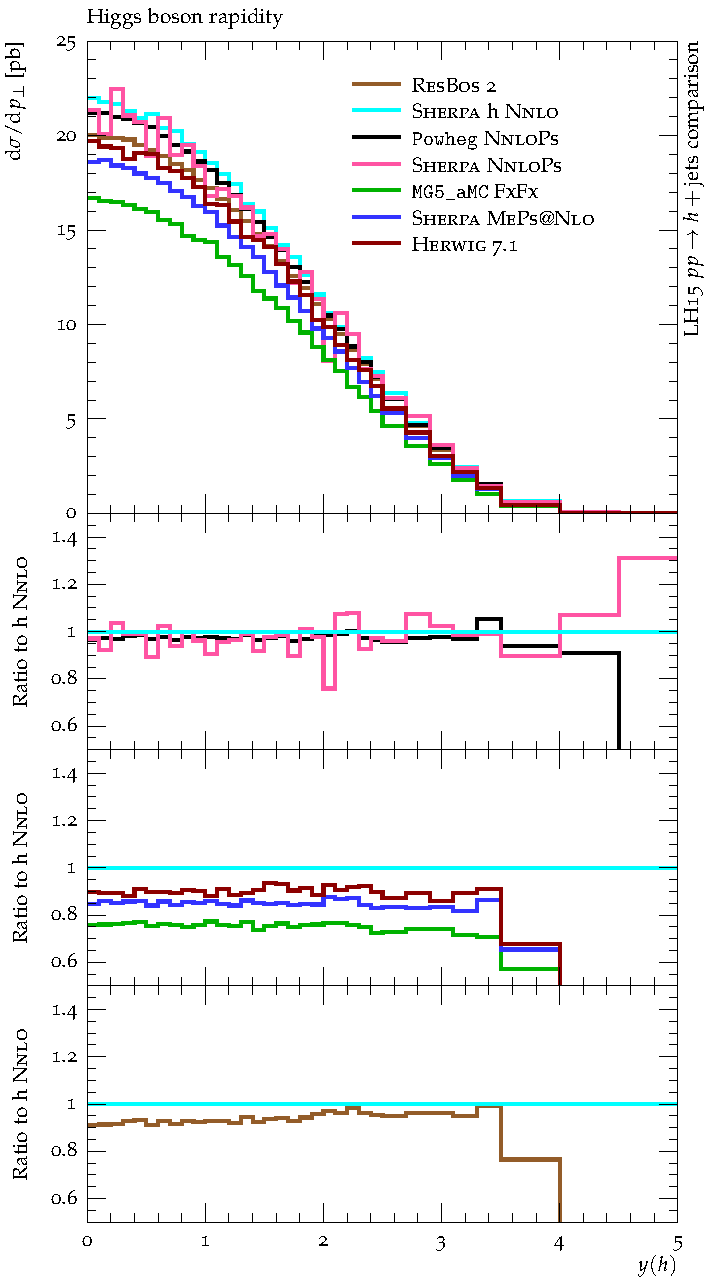
\includegraphics[width=0.47\textwidth]{figures/hjetscomp_u_H_y.pdf}
  \hfill
  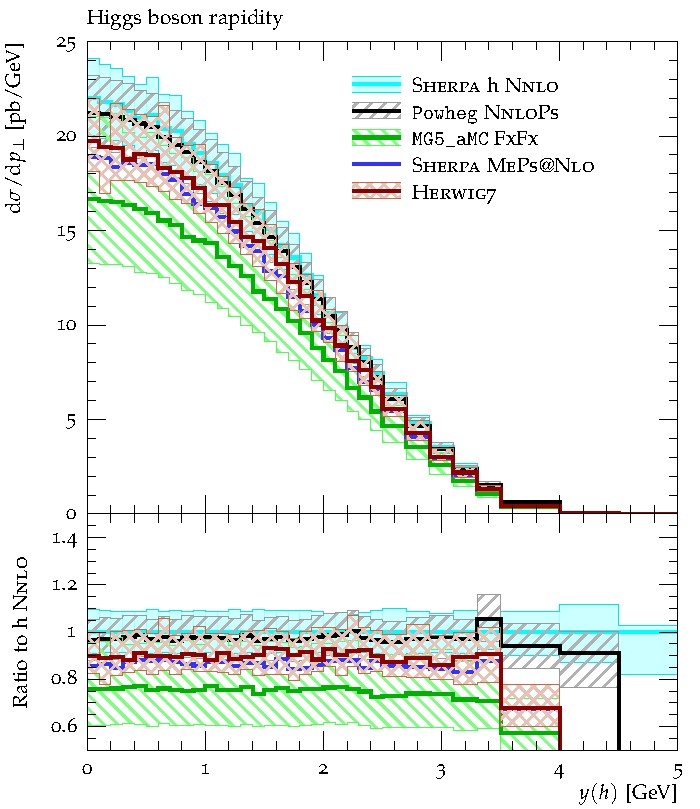
\includegraphics[width=0.47\textwidth]{figures/hjetscomp_H_y.pdf}
  \caption{\label{fig:hjetscomp:results:inclobs:hy}%
    The inclusive Higgs boson rapidity without (left) and with (right)
    uncertainties. To enhance visibility, the \NNLOPS, \MEPSatNLO and
    analytic $q_\text{T}$-resummation predictions are grouped together and
    shown with respect to the same reference curve in the upper, lower
    and middle ratio plots, respectively. The reference prediction is
    taken from the NNLO-accurate description of inclusive $h$ production.}
\end{figure}

We start by examining the inclusive Higgs boson rapidity distribution in
Figure~\ref{fig:hjetscomp:results:inclobs:hy}. While the absolute
predictions are given in the top panel, the plots in the bottom panel
depict the respective ratios to the NNLO prediction. For better
visibility, we have divided the predictions into three groups based on
their simulation type and/or claimed accuracy. The upper ratio plot
contains the NNLO predictions, while the middle ratio plot shows predictions obtained
from different strategies for  merging matrix elements plus parton showers
at NLO. The lower ratio plot displays the comparison between the pure
NNLO prediction and the matched result from \Resbos that includes the
effects from the $q_\text{T}$-resummation. Overall, we find very good
agreement in the description of the shape of the Higgs boson rapidity
distribution. The main source of deviations stems from the different
normalizations given at NNLO or NLO and the different (core) scale
choices. As expected, the \Sherpa \NNLOPS and
\Powheg \NNLOPS results agree well with the fixed-order NNLO prediction. 
The larger fluctuations found for \Sherpa \NNLOPS wrt.~\Powheg \NNLOPS
stem from the fact that the former is computed directly rather than
reweighted from an NLO computation for $hj$ final states.
\Resbos predicts a slightly smaller rate for $y(h)<2$ and a
slightly larger rate for $2<y(h)<3.5$ than the one given by the NNLO
calculation. The \MGaMC, \Sherpa \MEPSatNLO and \Herwig have slightly
lower (NLO) normalizations. Here, the \MGaMC scale choice reducing to
$m_h$, rather than $\tfrac{1}{2}m_h$, is clearly noticeable. The upper edge of
the \MGaMC uncertainty band (equal to a scale that reduces to $\tfrac{1}{2}m_h$)
agrees with the central value of the other NLO ME+PS
predictions. There are no major differences in the size of the
uncertainty envelopes, although to some extent, the NNLO scale
uncertainty bands (including \Resbos) are smaller than those at NLO,
as expected. Note
that the NLO-based predictions fall off more rapidly at higher $y$
than the NNLO-based predictions do. This is expected because of the
influence of additional $\ln(1-x)$ corrections present in the
determination of NNLO PDFs. Similar effects can be observed in going
from LO to NLO.

\begin{figure}[t!]
  \centering
  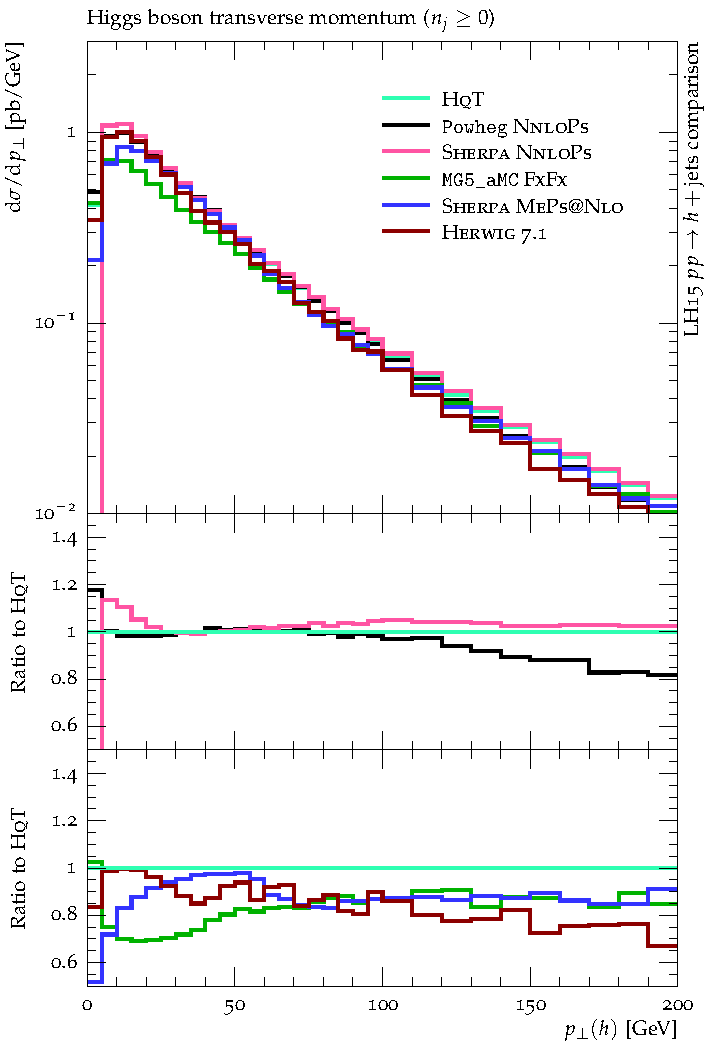
\includegraphics[width=0.47\textwidth]{figures/hjetscomp_u_H_pT_incl.pdf}
  \hfill
  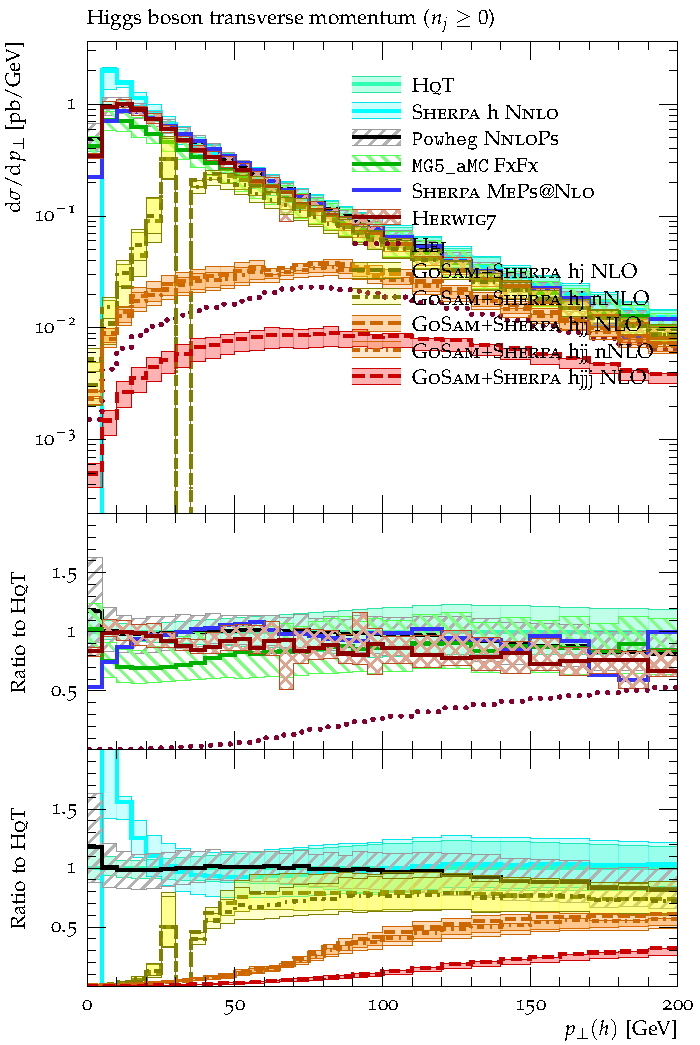
\includegraphics[width=0.47\textwidth]{figures/hjetscomp_H_pT_incl.pdf}
  \caption{\label{fig:hjetscomp:results:inclobs:hpt}%
    The Higgs boson transverse momentum in the inclusive event
    selection without (left) and with (right) uncertainties. For the
    ratios in the bottom panel, the same grouping strategy has been
    used as in Figure~\ref{fig:hjetscomp:results:inclobs:hy}, while
    the reference prediction has been changed from that of pure NNLO
    to the one as given by \HqT.}
\end{figure}

\begin{figure}[t!]
  \centering
  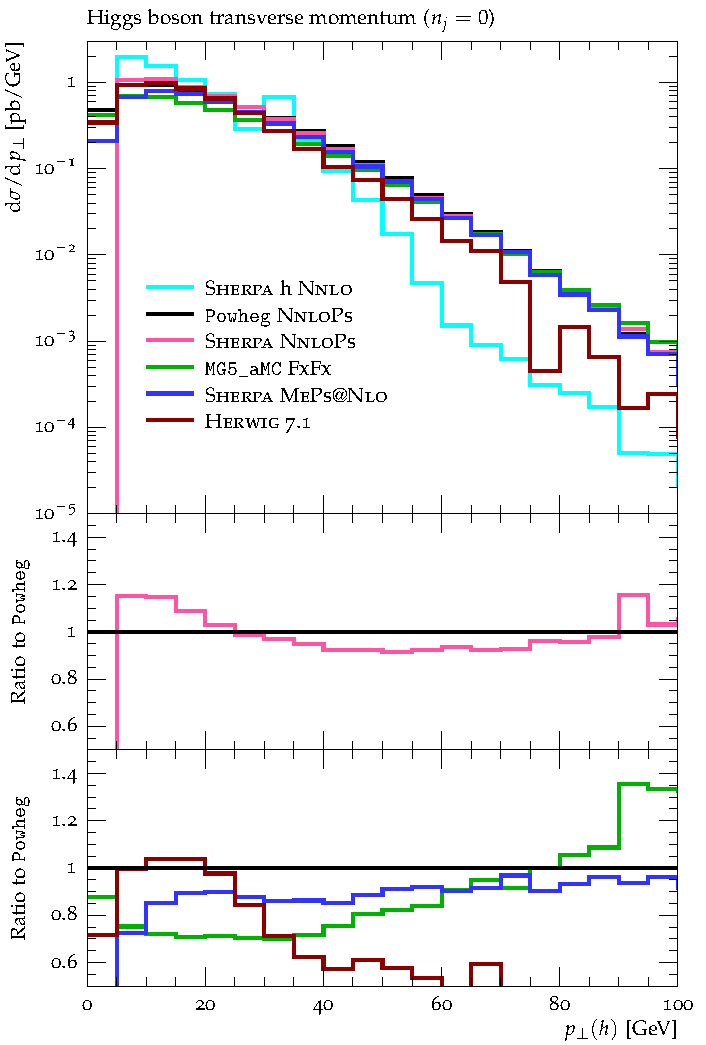
\includegraphics[width=0.47\textwidth]{figures/hjetscomp_u_H_pT_excl.pdf}
  \hfill
  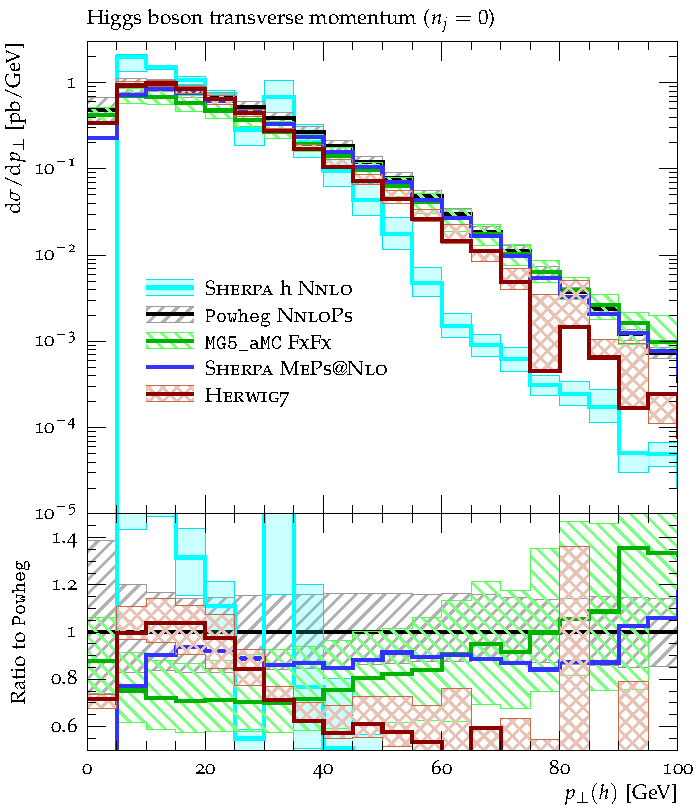
\includegraphics[width=0.47\textwidth]{figures/hjetscomp_H_pT_excl.pdf}
  \caption{\label{fig:hjetscomp:results:exclobs:hpt}%
    The Higgs boson transverse momentum in the exclusive event
    selection (i.e.~in the absence of any jet) without (left) and with
    (right) uncertainties. The  panels have been arranged as in
    the previous figure, apart from dropping the last panel,  and
    switching to a new reference curve  obtained from
    \Powheg \NNLOPS.}
\end{figure}

In Figures~\ref{fig:hjetscomp:results:inclobs:hpt} and
\ref{fig:hjetscomp:results:exclobs:hpt}, the inclusive and exclusive
(i.e.~vetoing events with jets above $30$\gev) Higgs boson transverse momentum
distributions are shown, respectively.  For the former, the ratios in
the bottom panels are taken with respect to the \HqT result, while
\Powheg \NNLOPS serves as the reference for the latter case. In
general, good agreement is found, with differences being somewhat more
pronounced in the exclusive case. For the inclusive version of the
$p_\perp(h)$ observable,  good agreement is observed with \HqT,
with some larger deviations evident at very low $p_\perp$. Here, the
resummation properties of the different parton showers dominate the
spectra of the matched and merged predictions. While at low $p_\perp$
the \Sherpa \NNLOPS curve starts about 15\% higher than both \HqT and
\Powheg \NNLOPS, it approaches the \HqT results at higher $p_\perp$.
The \Powheg \NNLOPS  prediction follows 
\HqT closely up to $p_\perp$ values of $\sim m_h$. The differences 
observed beyond that value are due to the 
dynamical scale choice employed by \Powheg \NNLOPS. The multijet merged calculations, due to their
similar scale choices, follow the pattern of the \Powheg \NNLOPS
prediction. Note that the differences in \MGaMC's central scale
choice becomes less significant as the Higgs boson transverse momentum
increases. \Herwig clearly provides the softest spectrum and \Sherpa
as well as \MGaMC predict a noticeably different shape for the Sudakov
suppression at low $p_\perp$, which is not covered by the \HqT
uncertainty envelope. For \Sherpa, the more significant suppression of
the lowest $p_\perp$ values can be traced back to the performance of the
\textsc{Csshower} which tends to radiate more strongly in this region.
The third ratio plot finally presents the direct comparison between
the two analytic resummation approaches, \HqT and \Resbos,
which are in good agreement with each other. The leftover
$\mathcal{O}(10\%)$ deviations between the two approaches can be
attributed to non-perturbative effects, still included in the latter, and the different handling of
the process-dependent pieces in the CFG and CSS schemes. The
\Resbos scale variation band features a cross-over point at
$p_\perp(h)\approx20\gev$ but this does not indicate or imply a
vanishing uncertainty at this point.
Lastly, we refrain from showing any fixed-order prediction here
because they are neither stable nor reliable at low $p_\perp$ in the
Sudakov region where resummation effects play a dominant role.

As shown in Figure~\ref{fig:hjetscomp:results:exclobs:hpt}, the
exclusive version of  the Higgs boson $p_\perp(h)$ distribution exhibits deviations among the
predictions that are more sizable. The $p_\perp(h)$ distribution 
declines much faster, easily spanning three orders of magnitude 
between zero and $100\gev$. This observable is less straightforward 
than the inclusive $p_\perp$-spectrum, as not only do Sudakov effects 
dominate the low-$p_\perp$ region, but resummation effects are also 
entering through the veto on any jet activity. A reliable description
of the observable therefore necessitates both a proper understanding
of the small $p_\perp(h)$ region and of jet production. Thus,
this is a stringent test of all predictions combining matrix elements
and parton showers (ME+PS), as
the high transverse momentum of the Higgs boson is produced by a
combination of soft jets (those that are below the $30$\gev threshold)
and soft gluon radiation. Note that the comparison is now taken with respect to
\Powheg \NNLOPS. The inclusive 
NNLO calculation is shown for this case in order  to demonstrate the failure of a fixed-order 
calculation on both accounts; thus, only the parton showered 
predictions are included in the study of the respective differences. 
Among them, apart from the differences already seen in the inclusive 
spectrum, both \NNLOPS calculations agree  well with one another, 
remaining within the 20\% uncertainty bands throughout the spectrum. 
While the \Sherpa \MEPSatNLO prediction remains mostly flat with respect to the \NNLOPS 
predictions, both \MGaMC and \Herwig exhibit shape differences  at
larger transverse momenta. In the case of \Herwig, the deviations  grow
larger than 40\%. From the resummation (i.e.~parton-shower)
point-of-view, all predictions are at a similar level here, although
formally the \NNLOPS techniques should lead to a more accurate description of
the exact zero-jet bin. The NLO merging approaches reduce to an \NLOPS
treatment in this zero-jet bin. It is however hard to infer this
formal difference from the behavior of the scale variation bands as
they are very comparable in size among all predictions. We conclude
that the deviation of the predictions probably provides us with a
better reflection of the true uncertainty.

\begin{table}[t!]
  \centering
  \begin{tabular}{c||c|c|c}
    Order \vphantom{$\int\limits_a^b$} &
    $\mu_\mathrm{R}=\mu_\mathrm{F}=\tfrac{1}{2}\,m_h$ &
    $\mu_\mathrm{R}=\mu_\mathrm{F}=\tfrac{1}{2}\,\sqrt{\vphantom{\big[}\Sigma_T}$ &
    $\mu_\mathrm{R}=\mu_\mathrm{F}=\tfrac{1}{2}\,\hat{H}_T'$ \\
    \hline\hline
    NLO \vphantom{$\int\limits_a^b$} &
    $17.0^{+3.0}_{-2.9}~\mathrm{pb}$ &
    $16.2^{+3.1}_{-2.8}~\mathrm{pb}$ &
    $13.5^{+2.0}_{-2.1}~\mathrm{pb}$ \\\hline
    NNLO \vphantom{$\int\limits_a^b$} & -- & $16.4^{+0.0}_{-0.9}~\mathrm{pb}$ & -- \\
    \hline
  \end{tabular}
  \caption{\label{tab:H1jXS}%
    The total cross section for the inclusive production of a Higgs
    boson and one additional jet using different core scale choices.
    The two dynamical scales are $\Sigma_T=m_h^2+\sum_\mathrm{jets}p_T^2$, see also
    Eq.~\eqref{eq:bfglpScale}, and
    $\hat{H}_T'=m_{T,h}+\sum_\mathrm{partons}p_T$,
    see also Eq.~\eqref{eq:hthatprime}. We note that though the NNLO figures
    are not available for $\tfrac{1}{2}\,\hat{H}_T'$ or $\tfrac{1}{2}m_h$, the variations
    will be very small.}
\end{table}

\begin{figure}[t!]
  \centering
  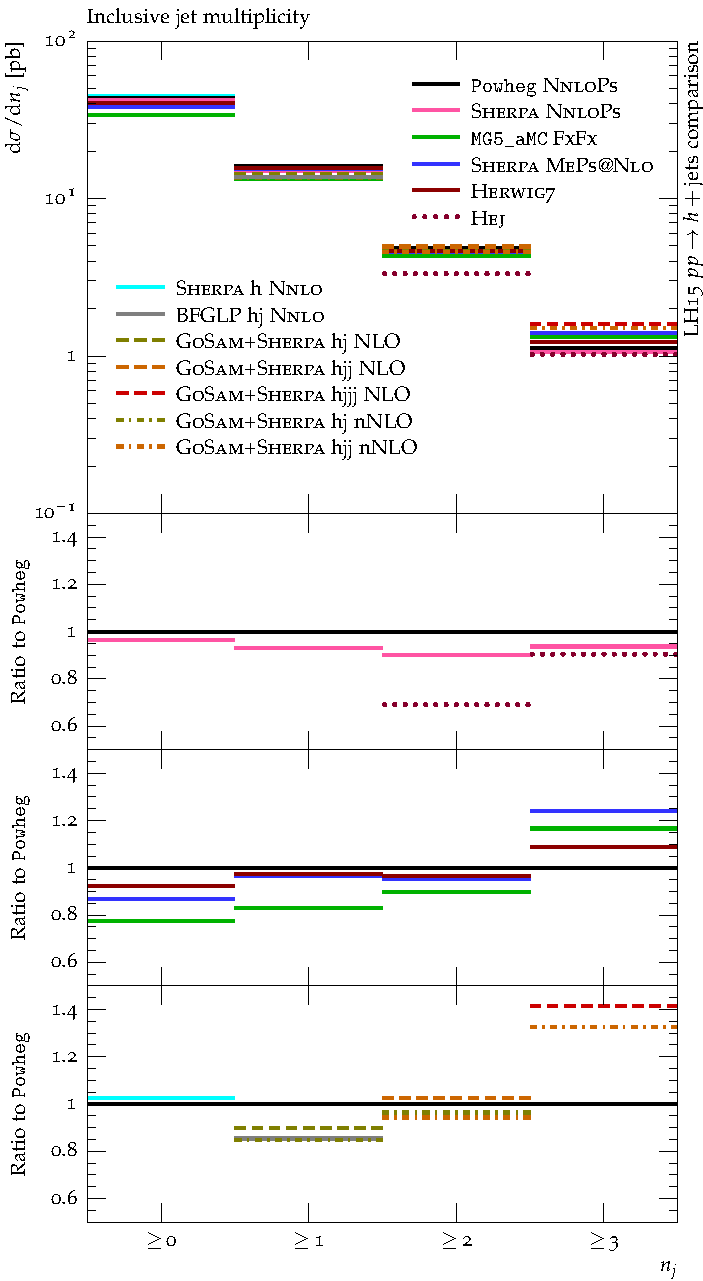
\includegraphics[width=0.47\textwidth]{figures/hjetscomp_u_NJet_incl_30.pdf}
  \hfill
  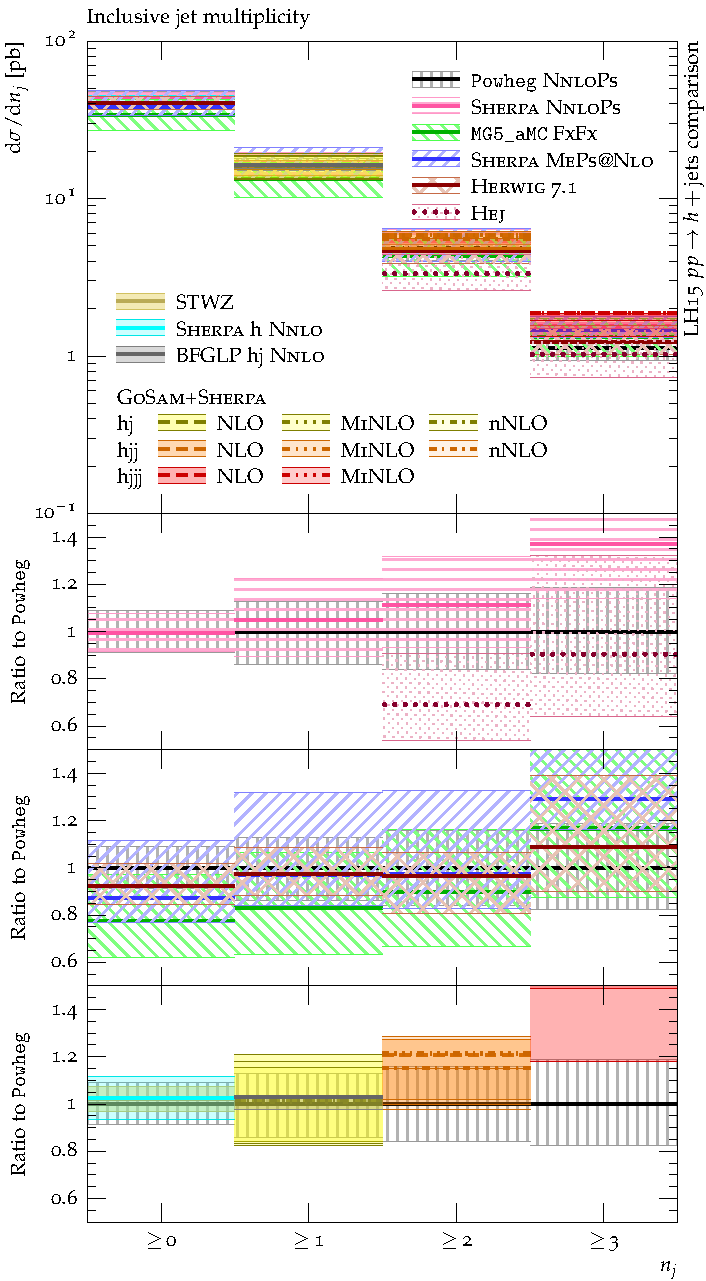
\includegraphics[width=0.47\textwidth]{figures/hjetscomp_NJet_incl_30.pdf}
  \caption{\label{fig:hjetscomp:results:inclobs:njets}%
    The central predictions on their own (left panel) and including their
    theoretical uncertainties (right panel) for the inclusive jet
    multiplicities as predicted by fixed-order calculations, resummed
    calculations, NNLO and NLO Monte Carlos. The bottom panel is
    divided up into three subplots all showing the ratios with respect
    to the \Powheg \NNLOPS prediction. The upper of these plots
    contains the \Hej and \Sherpa \NNLOPS ratios, while the middle one
    includes all NLO merged predictions (\MGaMC, \Herwig and \Sherpa)
    and the lower one shows all those listed in the bottom left legend
    of the main panel.}
\end{figure}

To obtain a first impression of how the different predictions 
compare beyond the zero-jet bins ($n_j\ge0$ and $n_j=0$), we now
examine the various inclusive and exclusive $n_j$ cross sections.
Accordingly, Figures~\ref{fig:hjetscomp:results:inclobs:njets} and
\ref{fig:hjetscomp:results:inclobs:njets_excl}, respectively, show the
inclusive ($n_j\ge N$) and the exclusive ($n_j=N$) jet multiplicity
distributions up to $N=3$, requiring \antikt jets
with $p_\perp>30\gev$. Two statements can be made before discussing
the individual results in more detail:
first of all, the agreement between all results is basically very good, and
second, the level of agreement is barely altered for exclusive jet
predictions compared to the inclusive jet predictions. 
Although not
shown here, when  the minimum jet-$p_\perp$ threshold is increased to
$50\gev$ the picture does not change significantly.
Again, the bottom panels are split up into several ratio plots with
the common reference provided by the \Powheg \NNLOPS result. The
upper ratio plot depicts the \NNLOPS methods together
with \Hej, which provides predictions only starting at $N=2$. Due to the similar core scale
choices in either \NNLOPS calculation, they share a common fully
inclusive cross section, with \Sherpa being greater than \Powheg for higher
jet multiplicities. Conversely, \Hej undershoots by 30\% in the
two-jet bin; however, this bin is described with an accuracy no higher
than LO by all predictions in this upper panel. In the three-jet bin
($N=3$), \Hej retains  LO accuracy, while both \NNLOPS calculations
produce this cross section by their respective parton showers
only. It is thus natural to find the largest differences between the
\NNLOPS predictions for $N=3$. Please note that the respective parton
shower uncertainties are partially incorporated in the \Sherpa \NNLOPS
uncertainty estimate, while they are not assessed for \Powheg,
resulting in a rather slowly increasing uncertainty band for rising
$N\le n_j$. And, more surprisingly, the \Powheg band remains very flat
in the $N=n_j$ case. The central ratio plot
compares the NLO matched and merged predictions with each other and
against the common reference \Powheg \NNLOPS. All these predictions
claim NLO accuracy for $N=0,1,2$, and thus overlap well within
uncertainties, where the lower value for \MGaMC can again be attributed
to the different scale choice. Again, with the same scale choice, all of
the calculations should agree much better. For $N=3$, only the \Sherpa \MEPSatNLO
prediction retains NLO accuracy, while \MGaMC and \Herwig revert to LO
accuracy, which is nicely reflected in the sizes of the uncertainty estimates. 
Unsurprisingly, in the $N=3$ case, all three NLO merged calculations
predict larger cross sections with respect to the reference whose rate
is only given by the parton shower, i.e.~\Pythia.

\begin{figure}[t!]
  \centering
  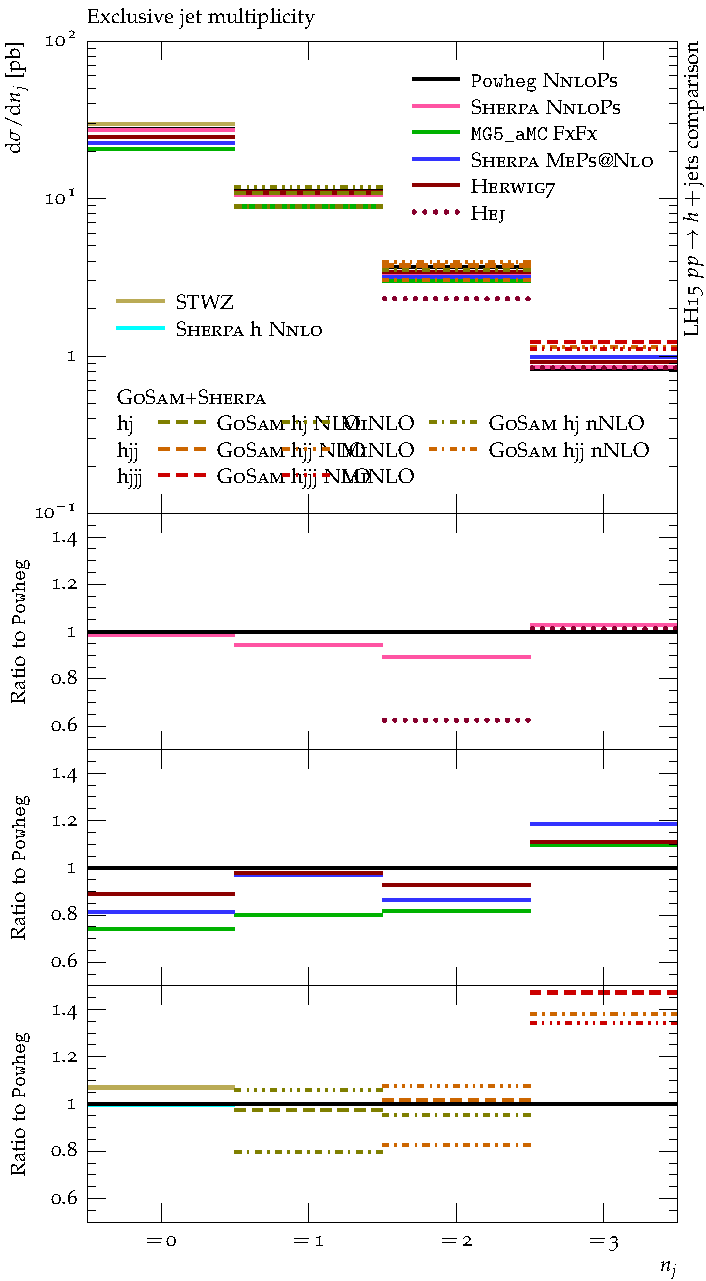
\includegraphics[width=0.47\textwidth]{figures/hjetscomp_u_NJet_excl_30.pdf}
  \hfill
  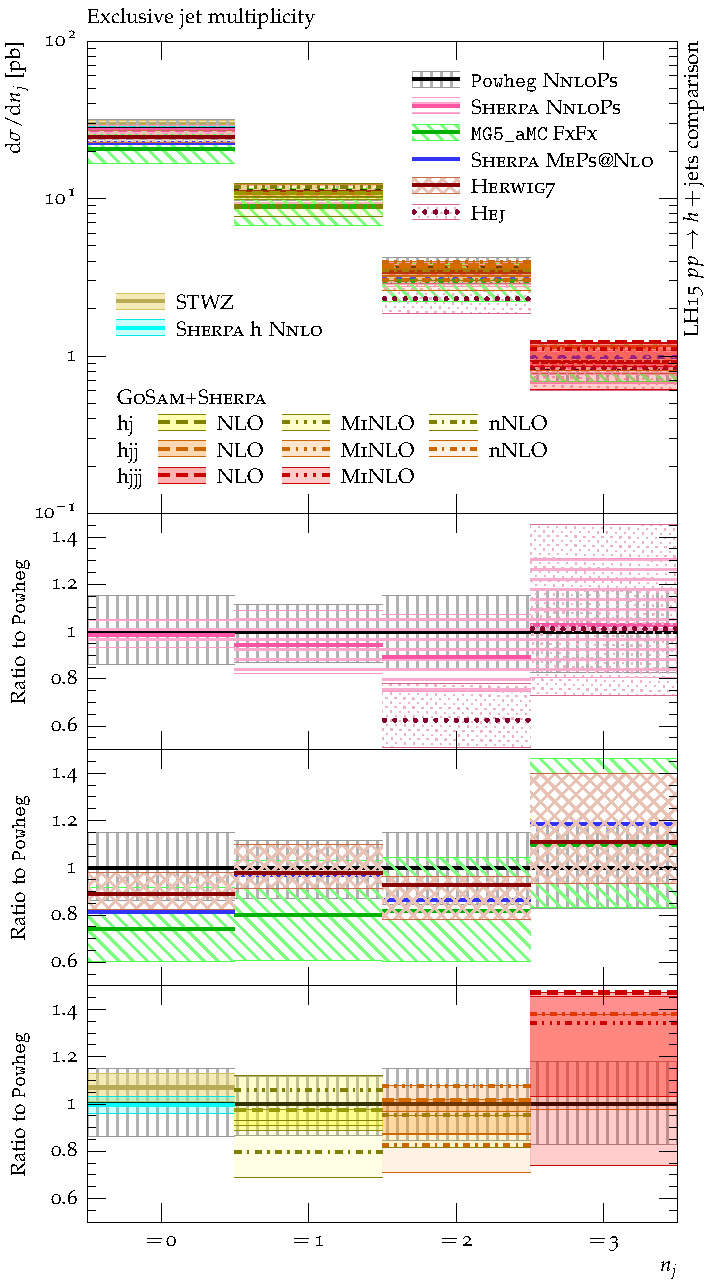
\includegraphics[width=0.47\textwidth]{figures/hjetscomp_NJet_excl_30.pdf}
  \caption{\label{fig:hjetscomp:results:inclobs:njets_excl}%
    The central predictions on their own (left panel) and including their
    theoretical uncertainties (right panel) for the exclusive jet multiplicities
    as predicted by fixed-order calculations, resummed calculations,
    NNLO and NLO Monte Carlos. The bottom panel is divided up into
    three subplots all showing the ratios with respect to the \Powheg
    \NNLOPS prediction. The upper of these plots contains the \Hej and
    \Sherpa \NNLOPS ratios, while the middle one includes all NLO
    merged predictions (\MGaMC, \Herwig and \Sherpa) and the lower one
    shows all those listed in the bottom left legend of the main panel.}
\end{figure}

Lastly, fixed-order predictions are shown for all jet multiplicities
at NLO (provided by \GoSam{}+ \Sherpa) for the $1$-jet, $2$-jet and
$3$-jet bins and at approximate NNLO (labeled nNLO, provided by \Loopsim) 
for the $1$-jet and $2$-jet bins.
Complete NNLO predictions are shown for the $0$-jet inclusive and
exclusive bins using \Sherpa (without PS), and for the $1$-jet inclusive
bin using the prediction of Boughezal et al.~(BFGLP).
The zero-jet bin comparison
also contains the resummation prediction of Stewart et
al.~(STWZ); the comparisons for non-zero jet bins also
include the \Minlo enhanced NLO calculations.
Figure~\ref{fig:hjetscomp:results:inclobs:njets} also
contains the \Resbos $q_\text{T}$-resummed predictions in the zero-jet bin
(with precision corresponding to NNLO+NNLL) as well as in the
one-jet bin (with precision corresponding to NLO+NLL). All of the
above are grouped together in the lower ratio plot.
For the zeroth bin, good agreement can be found between \Powheg and
\Sherpa $h$ NNLO as well as with the STWZ approach and \Resbos; the
uncertainties also are of comparable size, except for the
significantly wider $n_j=0$ envelope of \Powheg.
In the $1$-jet case, \Powheg (being NLO-accurate in this bin)
sits less than 3\% below the pure NLO prediction, with the small difference
being due to slightly different scale choices. Unlike the inclusive Higgs
boson production case, the NNLO corrections for inclusive $1$-jet
production are small (cf.~Table~\ref{tab:H1jXS})-- slightly positive
for the central scale choice as given in Eq.~\eqref{eq:bfglpScale}.
There is a notable decrease in the scale uncertainty with respect to
the NLO band given by \GoSam{}+\Sherpa. As expected, the uncertainty
envelope of the \Resbos prediction is of similar size while its
central value is about 5\% higher than the reference as a result of
its scale choice being $\mu=\tfrac{1}{2}m_h$.
The $2$-jet bin shows the \GoSam{}+\Sherpa NLO prediction 10-20\%
above \Powheg, which gives a LO prediction in this case. For the same
reason, we assume that the \Powheg uncertainties in the higher jet
multiplicities are probably underestimated.
In the $3$-jet bin (both inclusive and exclusive), the
\GoSam{}+\Sherpa and \Sherpa \MEPSatNLO predictions clearly indicate the
presence of  NLO corrections in the third jet bin. The \Loopsim
inclusive results for $hj$ and $hjj$ are always somewhat below the
respective \GoSam{}+\Sherpa results, and in the exclusive case this
difference gets more pronounced. However, the relatively large Monte
Carlo generation cut of $25\gev$ means that the total rates predicted
by \Loopsim should be interpreted with care.
Furthermore, compared to the NLO benchmark, the \Minlo approach
predicts 10-20\% larger cross sections for all non-zero jet bins.
Note that the \Minlo ratio for inclusive $hjjj$ turns out to be
outside the plot range appearing at around $1.65$, with the lower edge
of the uncertainty band at a ratio value of $1.5$.
In the cases where NNLO precision is available, the reduction in scale
uncertainty is clear. For $n_j\ge1$ the variation around
$\mu_\mathrm{R}=\sqrt{\Sigma_T}/2$ is about $5.5\%$ while for
$n_j\ge0$ it is about $10.0\%$ around $\mu_\mathrm{R}=\tfrac{1}{2}m_h$.
The latter result can be improved to only a few percent using the
N${}^3$LO prediction of Anastasiou et al.~\cite{Anastasiou:2015ema}.
In order to compare more easily with results presented previously in
the literature, we give numerical values at NLO and NNLO for different
scale choices in Table~\ref{tab:H1jXS}. As observed previously
\cite{Boughezal:2015dra}, the convergence of the total cross section predictions
is improved for scales that limit to $\tfrac{1}{2}m_h$. The dynamical
scale of $\sqrt{\Sigma_T}$ defined in Eq.~\eqref{eq:bfglpScale} is
slightly harder than the fixed scale given the minimum jet
$p_\perp(j)>30\gev$. On the other hand it is softer than $\hat{H}_T'$
defined in Eq.~\eqref{eq:hthatprime} which explains the differences observed at
NLO.



% =================

\begin{figure}[p!]
  %\vspace*{-50pt}
  \centering
  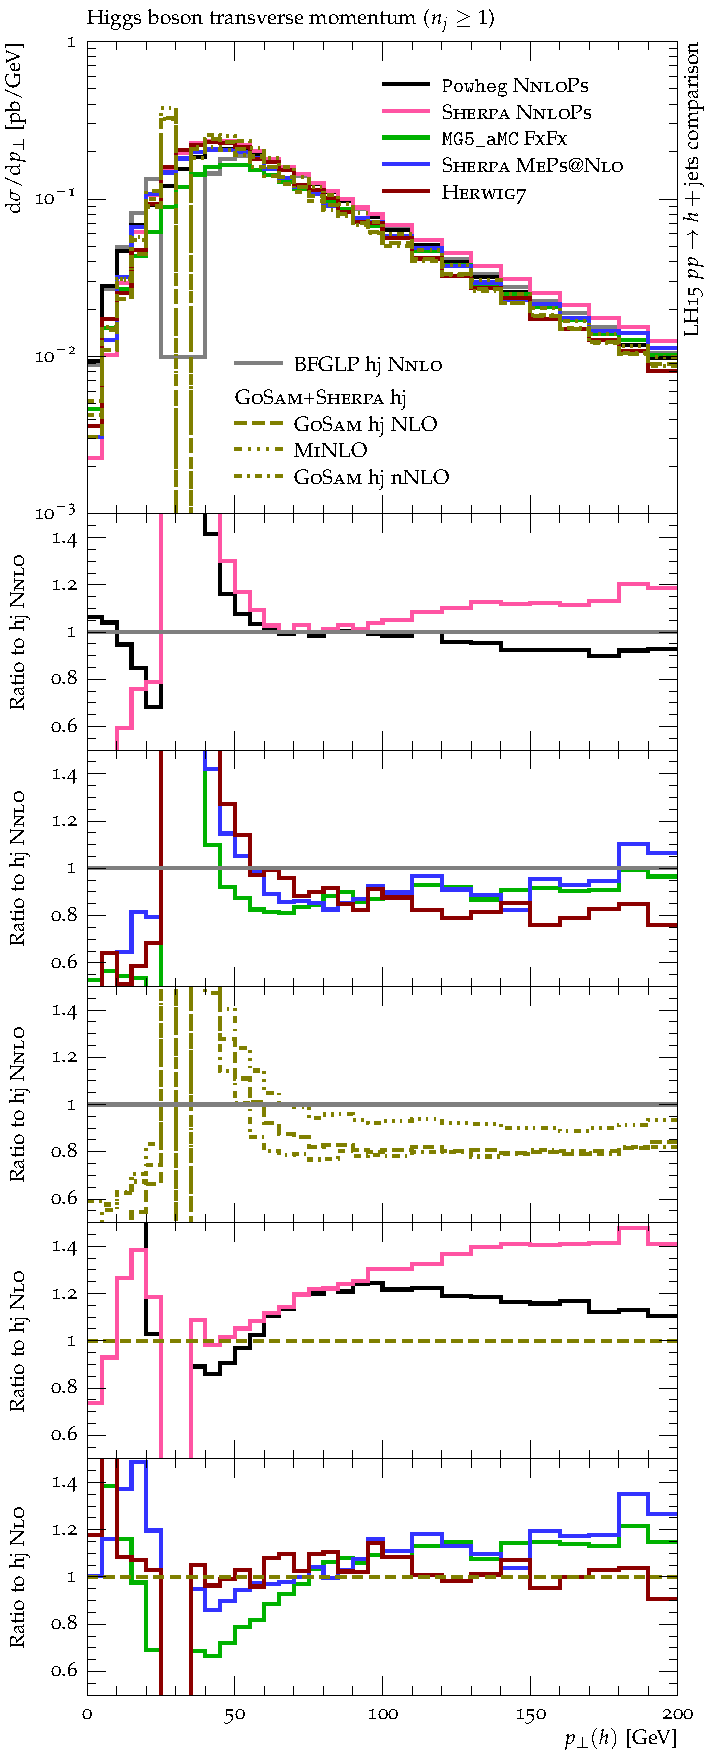
\includegraphics[width=0.47\textwidth]{figures/hjetscomp_u_H_j_pT_incl.pdf}
  \hfill
  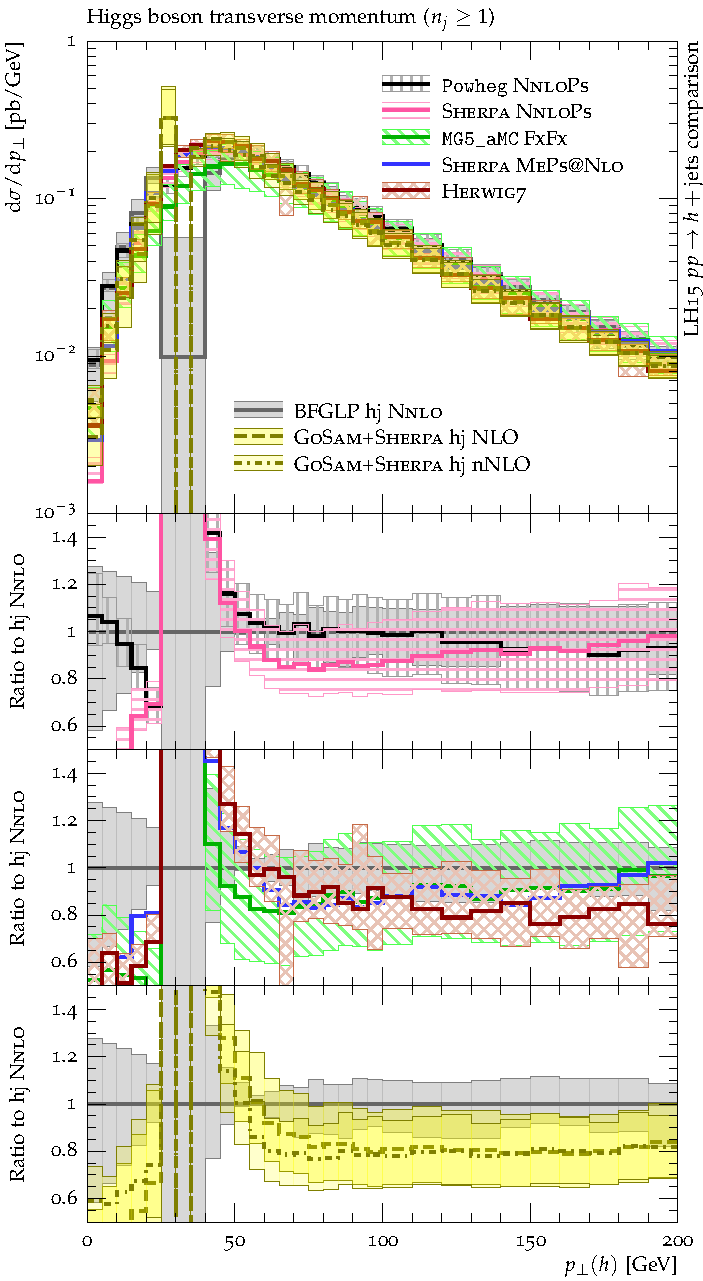
\includegraphics[width=0.47\textwidth]{figures/hjetscomp_H_j_pT_incl.pdf}
  \caption{\label{fig:hjetscomp:results:1obs:hpt}%
    The Higgs boson transverse momentum in the presence of at least
    one jet without (left) and with (right) uncertainty bands. The
    ratio plot panel is divided into six parts where the upper four
    exhibit the ratios wrt.~the \Powheg \NNLOPS result while the lower
    two show them wrt.~the NLO calculation for $h+1$~jet as
    provided by \GoSam{}+\Sherpa. The grouping in the ratio plots has
    been arranged to separately compare with each other the \NNLOPS
    predictions (first and fifth subplot), the NLO merging
    predictions (second and last subplot) and the fixed-order
    predictions (third subplot in the middle).}
\end{figure}

\begin{figure}[t!]
  \centering
  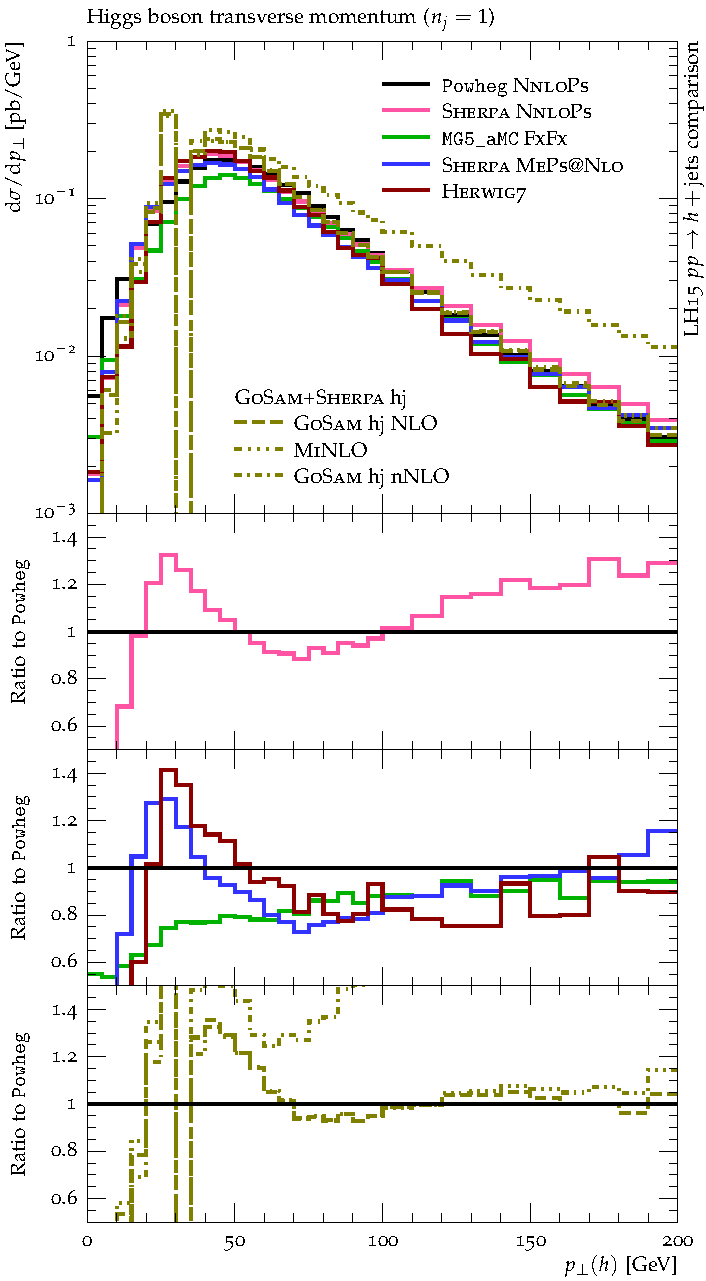
\includegraphics[width=0.47\textwidth]{figures/hjetscomp_u_H_j_pT_excl.pdf}
  \hfill
  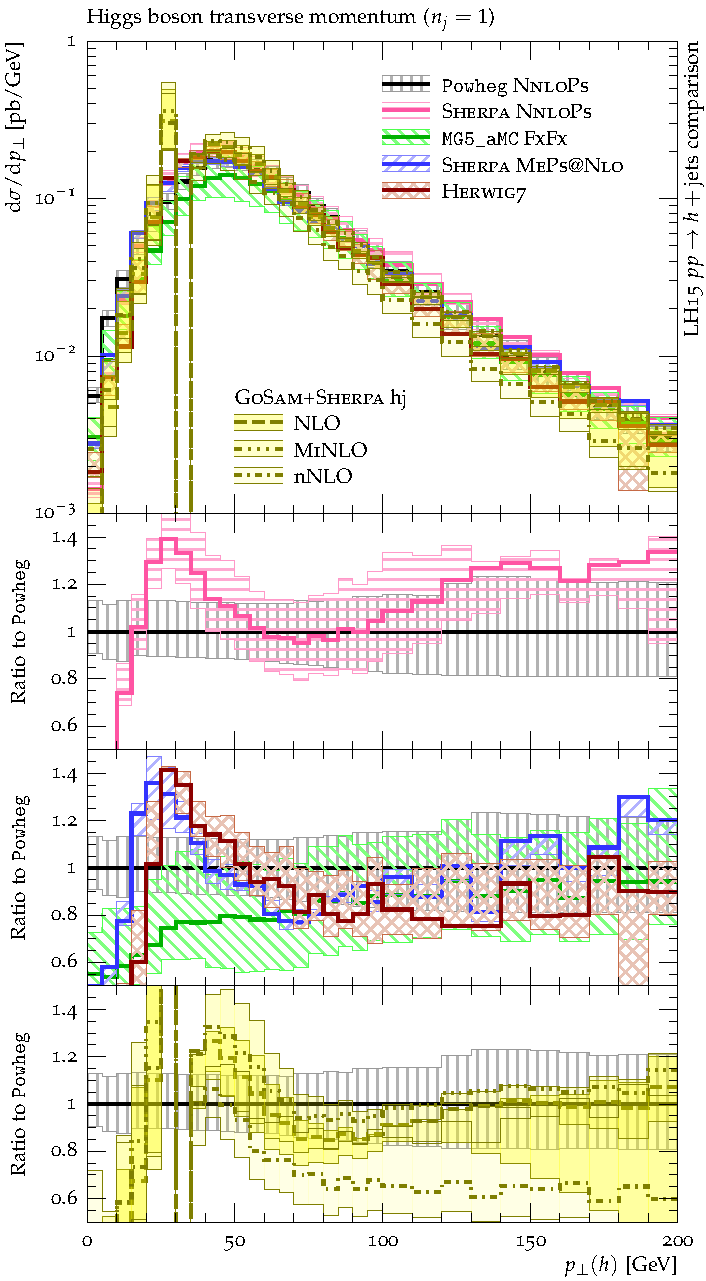
\includegraphics[width=0.47\textwidth]{figures/hjetscomp_H_j_pT_excl.pdf}
  \caption{\label{fig:hjetscomp:results:1obs:hpt_excl}%
    The Higgs boson transverse momentum in the presence of exactly one
    jet without (left) and with (right) uncertainty bands. The ratio
    plot panel is divided into three parts all of which depict the
    corresponding ratios wrt.~the \Powheg \NNLOPS result. From top to
    bottom, the predictions are grouped such that the \NNLOPS results,
    the ME+PS results at NLO and the fixed-order results are compared
    directly in the first, second and third ratio plot, respectively.}
\end{figure}


\subsubsection{One-jet observables}
\label{sec:hjetscomp:results:1jobs}

In this section, we move away from the fully inclusive picture and
require the presence of at least one jet associated with the Higgs
boson. In some cases we also ask for the predictions where exactly one
jet is being resolved. Recall that the jets are defined based on the
\antikt algorithm using $R=0.4$; they furthermore have to obey the
criteria that $p_\perp(j)>30\gev$ and $|\eta(j)|<4.4$. The set of
observables presented here includes the transverse momentum
distributions of the Higgs boson $h$, the leading jet $j_1$ and the
$hj_1$ two-body system as well as the rapidity spectrum of the leading
jet.

The Higgs boson transverse momentum distribution in the presence of at
least one jet is shown in
Figure~\ref{fig:hjetscomp:results:1obs:hpt}. The exclusive version of
this plot, i.e.~where one requires the Higgs boson and the jet to be 
the only resolved final state objects,
is presented in Figure~\ref{fig:hjetscomp:results:1obs:hpt_excl}. As
for the zero-jet cases discussed earlier in
Figures~\ref{fig:hjetscomp:results:inclobs:hpt}~and~\ref{fig:hjetscomp:results:exclobs:hpt},
the one-jet $p_\perp(h)$ variables are prone to large Sudakov effects that arise at low $p_\perp$, 
but are also present beyond
this region, in particular for the exclusive final states. Moreover, the
Sudakov shoulder effect can be observed for all fixed-order
predictions shown here. The jet-$p_\perp$ threshold leads to a
non-smooth behavior of the $p_\perp(h)$ observable at LO, and
therefore to the existence of a critical point at $30\gev$, for which
the cancellations between real and virtual soft-gluon singularities
will be imperfect at any given fixed, higher order in perturbation
theory~\cite{Catani:1997xc}. For the BFGLP $hj$ NNLO  prediction, an
averaging procedure has been used to dampen the effect around the jet
threshold, while for the NLO predictions, the large oscillations are a
clear indication of the instability emerging at the jet threshold. The
\NNLOPS, NLO ME+PS and \Resbos predictions do not suffer from
the Sudakov shoulder effect since they include the necessary all-order
resummation corrections.

Comparing the different fixed-order predictions, which are detailed in 
the third ratio plot, noticeable differences only
occur between the NNLO prediction and the four NLO predictions as
obtained from \Powheg and the three variations on \GoSam{}+\Sherpa (pure
NLO, \Minlo and \Loopsim). The NNLO tail is harder by about 15\% which
is expected since the $p_\perp$ tail is affected by multijet
contributions. The NNLO treatment includes these contributions to a
larger extent, as it includes $h+2$-jet and $h+3$-jet contributions at
 NLO and LO, respectively. For $p_\perp(h)<30\gev$, the (N)NLO
description is degraded to (N)LO. Here, the presence of the
$\mathcal{O}(\alpha_\mathrm{s})$ term of the Sudakov resummation, also
included in the NLL resummation of \Resbos, affects the BFGLP $hj$
NNLO calculation. However, it can also be noticed (see fourth ratio plot in
Figure~\ref{fig:hjetscomp:results:1obs:hpt}) that apart from the BFGLP
$hj$ NNLO calculation, \Resbos and also \Powheg, all other approaches
predict a more steeply falling shoulder resulting in a significantly
lower cross section as $p_\perp(h)\to0$.
For larger $p_\perp(h)$ values, $p_\perp(h)\gtrsim\tfrac{1}{2}m_h$, in
general there is good agreement between \Powheg, \MGaMC, \Sherpa
\MEPSatNLO and the NLO curves; this can be expected as these
predictions are all NLO-accurate. As before, \Herwig tends to be
softer, whereas \MGaMC, using the nominal $\tfrac{1}{2}m_h$ core scale,
turns out to be harder by almost 40\%, as indicated by the upper edge
of its corresponding uncertainty band (see the second or last subplot
to the right in Figure~\ref{fig:hjetscomp:results:1obs:hpt}). \Sherpa's
\NNLOPS prediction also features a harder tail than \Powheg owing to the
different scale setting procedures employed by the two approaches.
While in \Powheg the scale setting is accomplished through the \Minlo
procedure, \Sherpa's \NNLOPS uses the fixed scale choice of $\tfrac{1}{2}m_h$
and therefore enhances the $p_\perp$ tail with respect to \Powheg's
result. In this region, the \Resbos prediction closely resembles the
one given by \Sherpa \NNLOPS, since it is dominated by the fixed-order
contribution evaluated with the same scale choice as used in \Sherpa.

We furthermore observe that apart from the BFGLP $hj$ NNLO computation,
all uncertainty envelopes are of similar size. This does not come as
a surprise because all of these predictions are effectively given at
NLO. The NNLO uncertainty band (shown in grey) is found to be
significantly smaller. Comparing the second and last ratio plots with
each other, we also notice that the ME+PS predictions are in better
overall agreement with the pure NLO prediction given by
\GoSam{}+\Sherpa than they are in agreement with \Powheg, with the
exception of \MGaMC below $p_\perp(h)\lesssim\tfrac{1}{2}m_h$. This is
surprising since all parton shower matched calculations are of the
same intrinsic accuracy (NLO), use similar local scale definitions
along the lines of CKKW and include Sudakov factors of NLL accuracy.
It may, however, be related to the way the resummation is controlled
in \Powheg and the \MCatNLO-type matchings used in \MGaMC, \Herwig and
\Sherpa. The different parton shower starting scales employed in
\Herwig and \Sherpa ($\sim\tfrac{1}{2}m_h$), \MGaMC ($\sim m_h$) and
\Powheg ($E_\mathrm{cm}$) do also play a role.

For the exclusive one-jet case, we reduce the number of ratio plots
and show only those that display the ratios to \Powheg in the same way
as before. Note that for the exclusive version of the observable, the
NNLO result is not available, turning this comparison into one between
NLO-accurate predictions, except for the NNLO-approximate result given
by \Loopsim, labelled \GoSam{}+\Sherpa $hj$ nNLO.
Figure~\ref{fig:hjetscomp:results:1obs:hpt_excl} clearly shows that
the differences among the results are very similar to those discussed
in the inclusive case; they are however pronounced such that the
deviations wrt.~the \Powheg \NNLOPS prediction for $h$ production
become larger for the full tranverse momentum range. There is one
exception to this: \Loopsim predicts a softer tail of the $p_\perp(h)$
distribution by about 20\%, which in the end is a restatement of the
fact that there is a 20\% difference in the one-jet rate between the
pure NLO and the \Loopsim result, as already shown in
Figure~\ref{fig:hjetscomp:results:inclobs:njets_excl}.

\begin{figure}[t!]
  \centering
  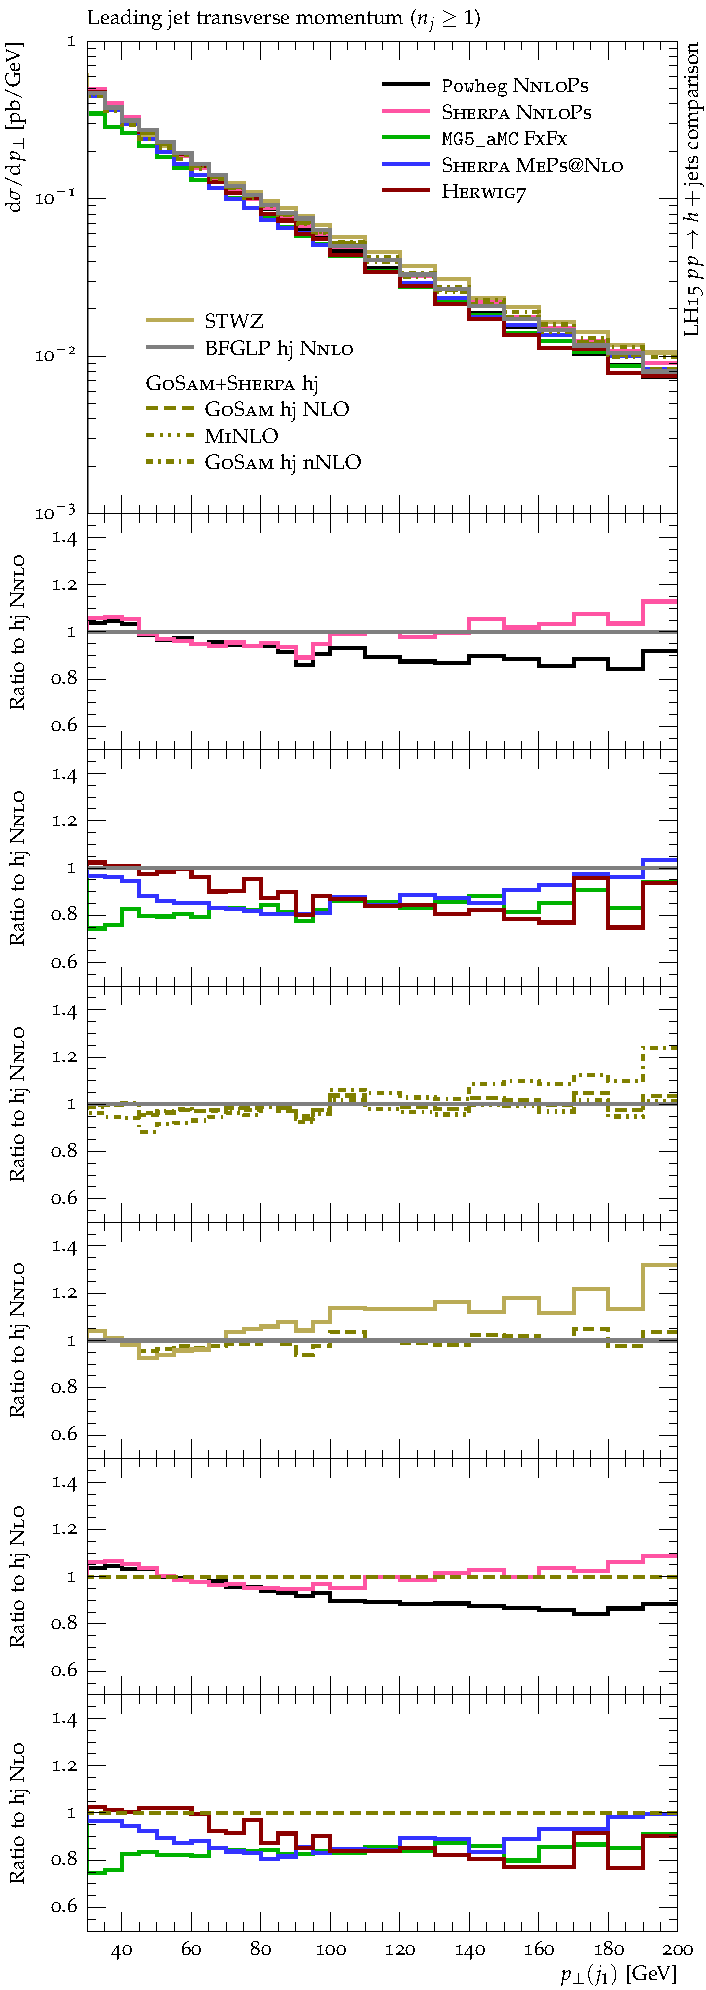
\includegraphics[width=0.47\textwidth]{figures/hjetscomp_u_jet1_pT_incl.pdf}
  \hfill
  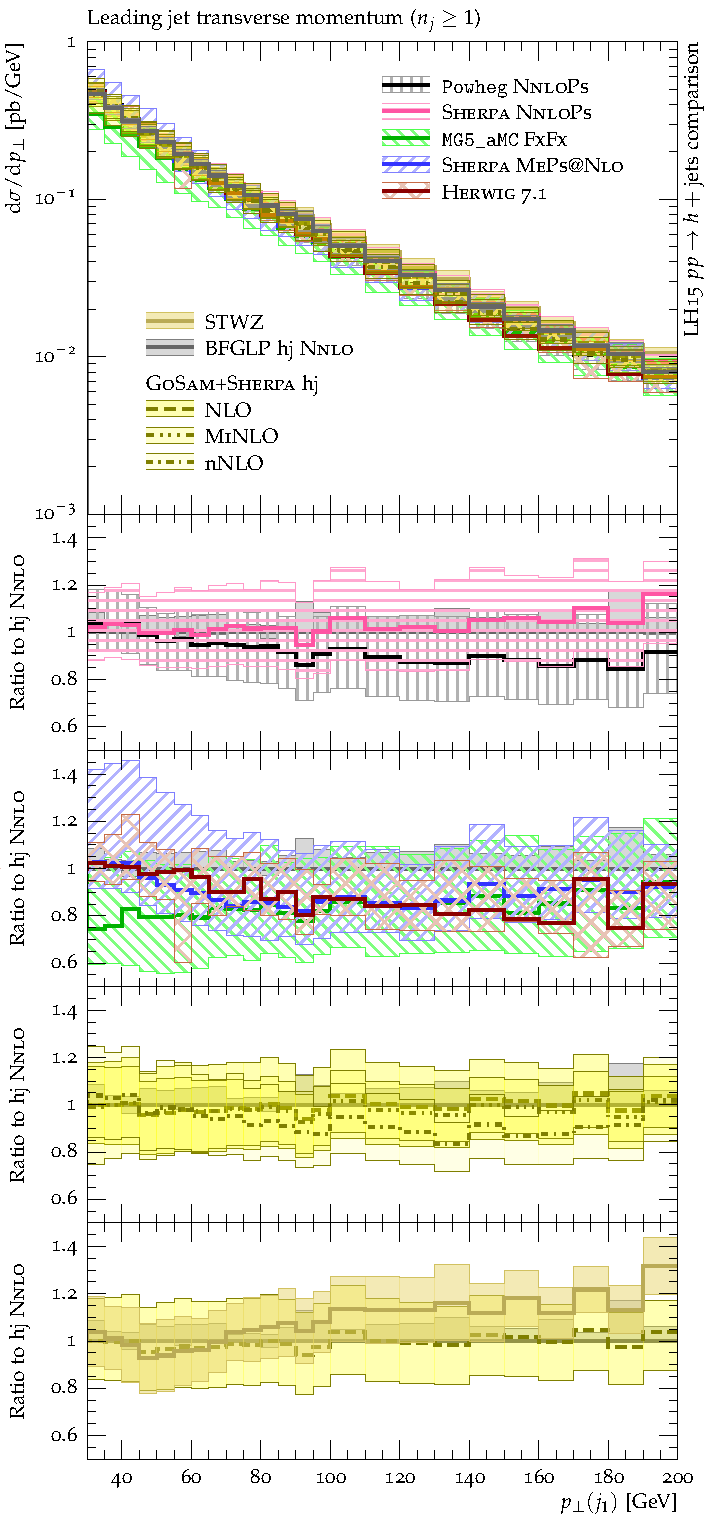
\includegraphics[width=0.47\textwidth]{figures/hjetscomp_jet1_pT_incl.pdf}
  \caption{\label{fig:hjetscomp:results:1obs:j1pt}%
    The leading jet transverse momentum distribution for
    $h\,+\!\ge\!1$-jet production, to the right (left) shown with
    (without) the uncertainty bands provided by the various
    calculations. The part below the main plot contains four ratio
    plots taken wrt.~the NNLO result of the BFGLP group following the
    same strategy for grouping the predictions as before (\NNLOPS
    versus NLO ME+PS versus fixed-order and resummation results).}
\end{figure}

\begin{figure}[t!]
  \centering
  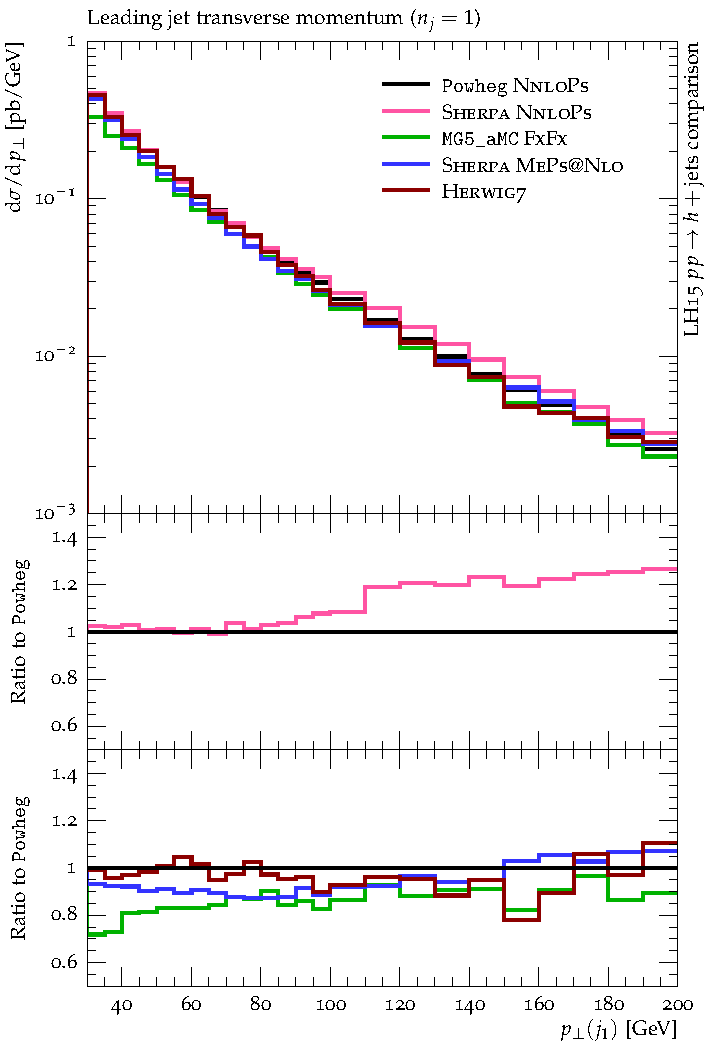
\includegraphics[width=0.47\textwidth]{figures/hjetscomp_u_jet1_pT_excl.pdf}
  \hfill
  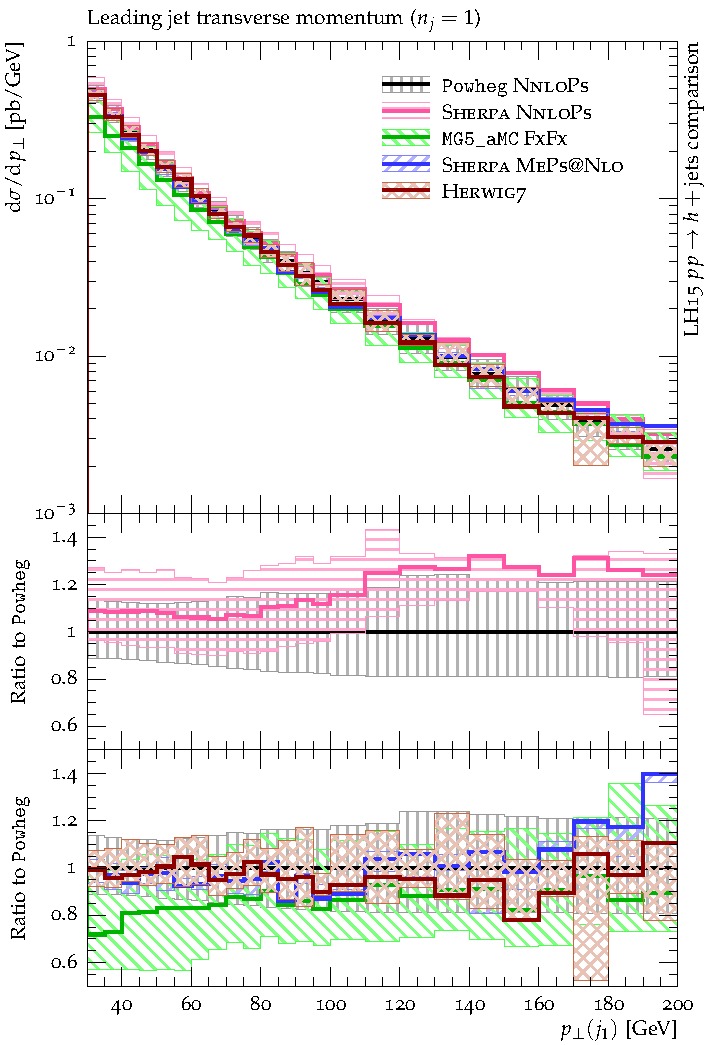
\includegraphics[width=0.47\textwidth]{figures/hjetscomp_jet1_pT_excl.pdf}
  \caption{\label{fig:hjetscomp:results:1obs:j1pt_excl}%
    The leading jet transverse momentum distribution for exclusive
    $h+1$-jet production, to the right (left) shown with (without)
    the uncertainty bands provided by the various calculations. Ratio
    plots are displayed in the lower part of the plot using the
    \Powheg \NNLOPS result for Higgs boson production as their
    reference. Predictions are grouped in similar fashion to the
    previous plots.}
\end{figure}

Next we discuss the leading jet transverse momentum distribution for
$h\,+\!\ge\!1$-jet final states. For this type of observable, we do
not expect large Sudakov effects (i.e.~shifts owing to parton
showering/resummation). The impact of jet veto logarithms (owing to
the restriction that all jets be greater than $30\gev$) has been
examined and found to be reasonably small at NLO and
NNLO~\cite{Banfi:2012jm,Banfi:2015pju}.
In the exclusive jet case, the $p_\perp(j_1)$ variable however is
prone to larger resummation effects, and we note that the scale
uncertainties shown will not reflect the true uncertainty. The
inclusive jet results for all approaches are shown in
Figure~\ref{fig:hjetscomp:results:1obs:j1pt} including the NNLO
prediction of the BFGLP group, the prediction of Stewart, Tackmann
et al.~and the prediction provided by \Resbos.
Figure~\ref{fig:hjetscomp:results:1obs:j1pt_excl} depicts the
exclusive one-jet case presenting the results obtained by the Monte
Carlo tools only; no fixed-order/resummation predictions are shown.
Accordingly, different reference predictions (NNLO and \Powheg) are
used in the ratio plots associated with
Figures~\ref{fig:hjetscomp:results:1obs:j1pt} and
\ref{fig:hjetscomp:results:1obs:j1pt_excl}. 
Overall we find a rather remarkable agreement
between all results where the largest deviations rarely exceed the
20\% mark. For the exclusive lead-jet transverse momentum distribution
of Figure~\ref{fig:hjetscomp:results:1obs:j1pt_excl}, this means that
all predictions are in reasonably good agreement with \Powheg. The
\MGaMC prediction is lower than \Powheg for almost the entire
transverse momentum range, again because of the central scale choice
being higher than in the other approaches. For the inclusive lead-jet
transverse momentum spectrum (see
Figure~\ref{fig:hjetscomp:results:1obs:j1pt}), the remarkable
agreement implies that all predictions indeed lie within each other's
uncertainty bands (as they should). The quoted uncertainties are similar in size, with
values at and around the 20\% level, and only those of the BFGLP $hj$
NNLO calculation are significantly smaller. 

\begin{figure}[t!]
  \centering
  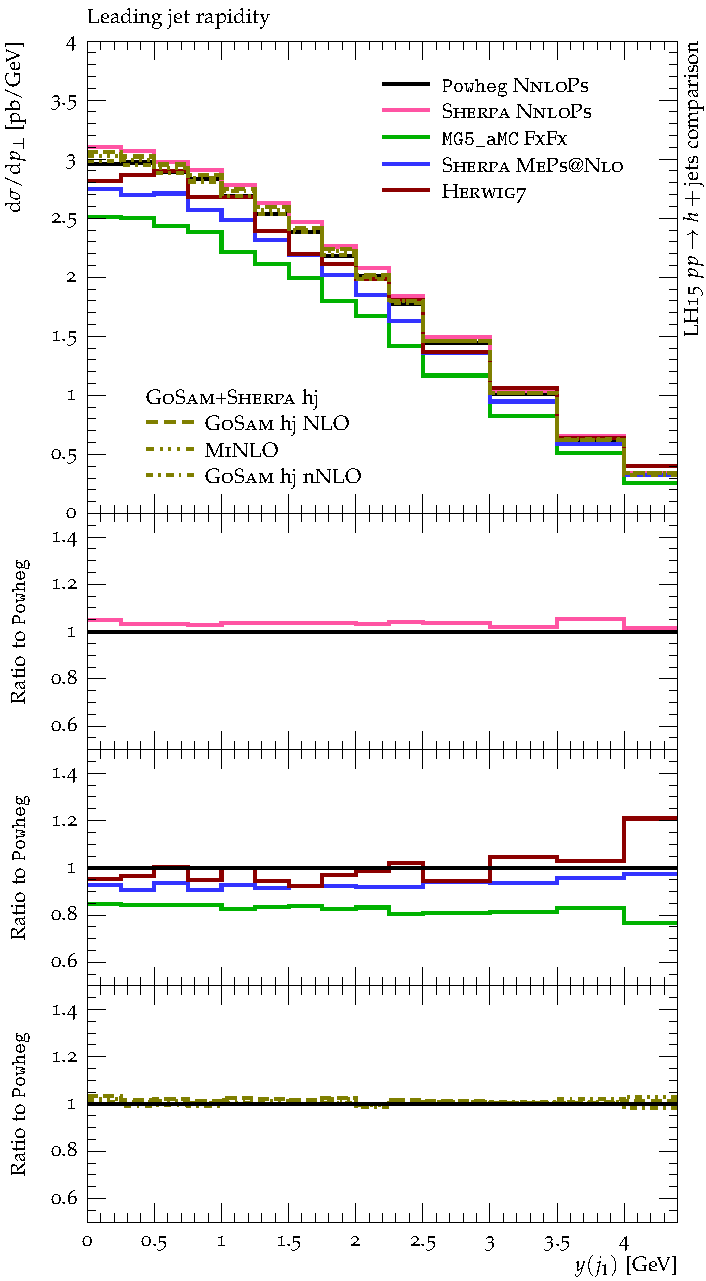
\includegraphics[width=0.47\textwidth]{figures/hjetscomp_u_jet1_y.pdf}
  \hfill
  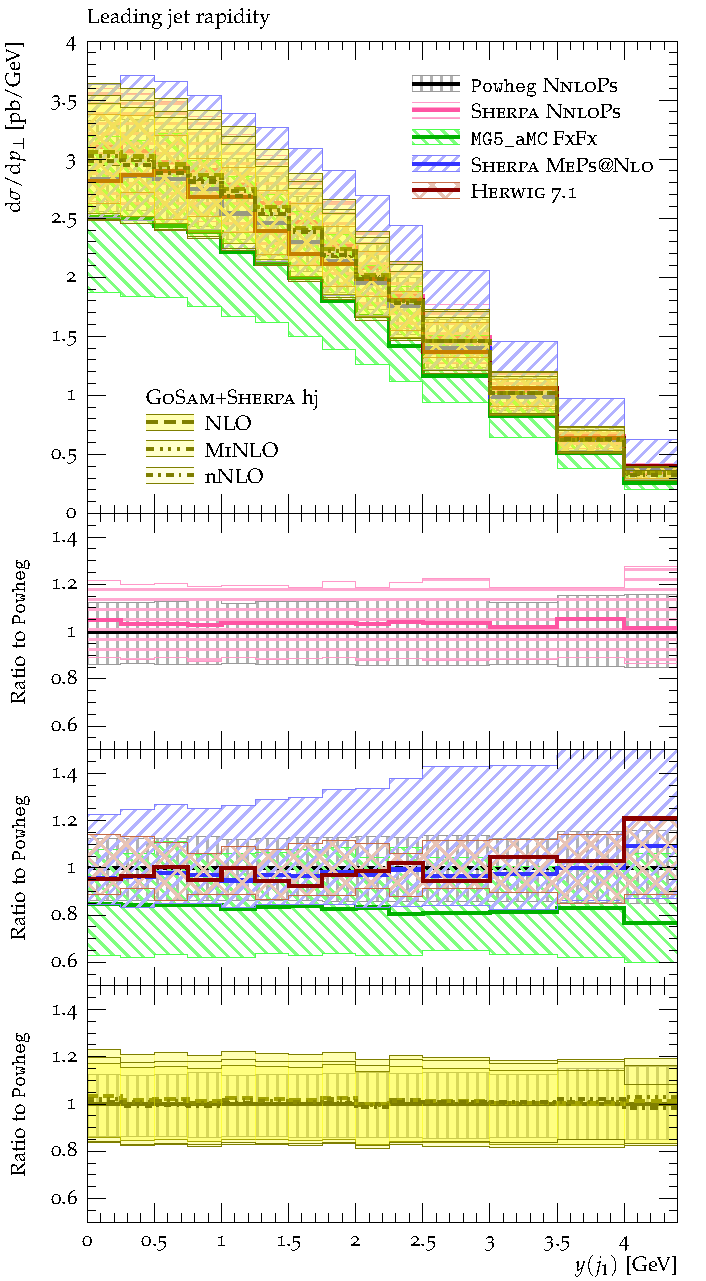
\includegraphics[width=0.47\textwidth]{figures/hjetscomp_jet1_y.pdf}
  \caption{\label{fig:hjetscomp:results:1obs:j1y}%
    The rapidity distribution for the leading jet in $h\,+\!\ge\!1$-jet
    production, shown without (left) and with (right) theoretical
    uncertainties. Ratio plots are displayed in the lower part of the
    plot using the \Powheg \NNLOPS result for Higgs boson production
    as their reference. Predictions are grouped, from top to bottom,
    according to the categories \NNLOPS, ME+PS at NLO and NLO fixed
    order as well as resummation.}
\end{figure}

Despite the good agreement seen among all predictions in
Figure~\ref{fig:hjetscomp:results:1obs:j1pt}, it is worthwhile to go
through the ratio plots and discuss some of the interesting features.
In the top ratio panel, the two \NNLOPS predictions are compared to the
NNLO $h\,+\!\ge\!1$-jet prediction. The agreement among all three is
good at low transverse momentum, but at higher $p_\perp(j_1)$ there is
a tendency for \Sherpa \NNLOPS to move to the upper edge of the NNLO 
uncertainty band and \Powheg \NNLOPS to move slightly below, resulting 
in a 20\% net difference between the two. Again, this is a result of using
$\mu=\tfrac{1}{2}m_h$ within \Sherpa versus using \Minlo/CKKW scales within the
\Powheg approach. In the second ratio panel, \Herwig, \Sherpa and \MGaMC
(taking into account its larger limit scale) agree reasonably well
with each other over the entire transverse momentum range, but fall
about 15\% low wrt.~the BFGLP prediction in the mid-range of the
$p_\perp$ distribution. The third ratio panel shows that there is almost no
difference in normalization nor shape between the NNLO and the NLO
$h\,+\!\ge\!1$-jet predictions using the given scale choice,
cf.~Eq.~\eqref{eq:bfglpScale}. This extends to the \Minlo reweighted
NLO result and the nNLO prediction provided by the \Loopsim approach,
although the latter is somewhat softer. Nevertheless we should bear in
mind that if we were to include in this comparison a fixed-order
calculation based on the scale choice $\tfrac{1}{2}\hat H_T^\prime$,
the resulting prediction would fall close to the multijet merged
predictions, showcasing the still largish scale dependence of the $hj$
NLO calculation. In the bottom ratio panel, the STWZ and \Resbos
predictions agree very well with one another, partly because in their
calculation they both rely on the same fixed-order piece dominating
this observable and coincide in their use of fixed scale. Both
approaches provide a resummation improved NLO calculation for this
observable, agreeing with the NNLO prediction at low $p_\perp$. At the
largest $p_\perp$ values, where no resummation effects are present,
deviations rise up to 30\% owing to their fixed scale choice, which
furthermore brings them into agreement with \Sherpa's \NNLOPS result.
As a matter of fact, for sufficiently large values of $p_\perp(j_1)$,
all three predictions converge to an NLO prediction employing a fixed
scale of $\mu=\tfrac{1}{2}m_h$.

In summary, the fixed-order NNLO prediction of the BFGLP group, which
has the best theoretical uncertainties available, is in good agreement
with the \Sherpa \NNLOPS prediction, and to a
somewhat lesser extent, with the \Powheg \NNLOPS predictions. The level of
moderate disagreements observed with the multijet merged calculations 
may be due to the different scale choices that are still important 
at NLO. The largest deviation seen with \MGaMC can mainly be traced
back to its different choice of central scales. There is no sign of
any serious impact of the merging of the fixed-order predictions with
parton showers, as expected for such an inclusive cross section.

Even better agreement is observed  for predictions for the rapidity distribution of the lead jet,
$y(j_1)$, as demonstrated by Figure~\ref{fig:hjetscomp:results:1obs:j1y}.
This level of agreement seems to be even slightly better than the one
found for $y(h)$ in Figure~\ref{fig:hjetscomp:results:inclobs:hy}.
We do not observe any shape differences, and the rate differences 
follow the already established pattern where most noticeably the
\MGaMC cross section is reduced owing to their choice of using a
higher central scale. Similarly, \Sherpa \NNLOPS and \Resbos are
higher by about 6-7\% as a result of using the fixed scale
$\mu=\tfrac{1}{2}m_h$. Again, uncertainty envelopes are similar in
size and do not point to any shape changes when varying the scales;
\Herwig's band is slightly narrower while \Sherpa \MEPSatNLO's and
\MGaMC's band are somewhat wider compared to all other NLO-accurate
predictions.

\begin{figure}[t!]
  \centering
  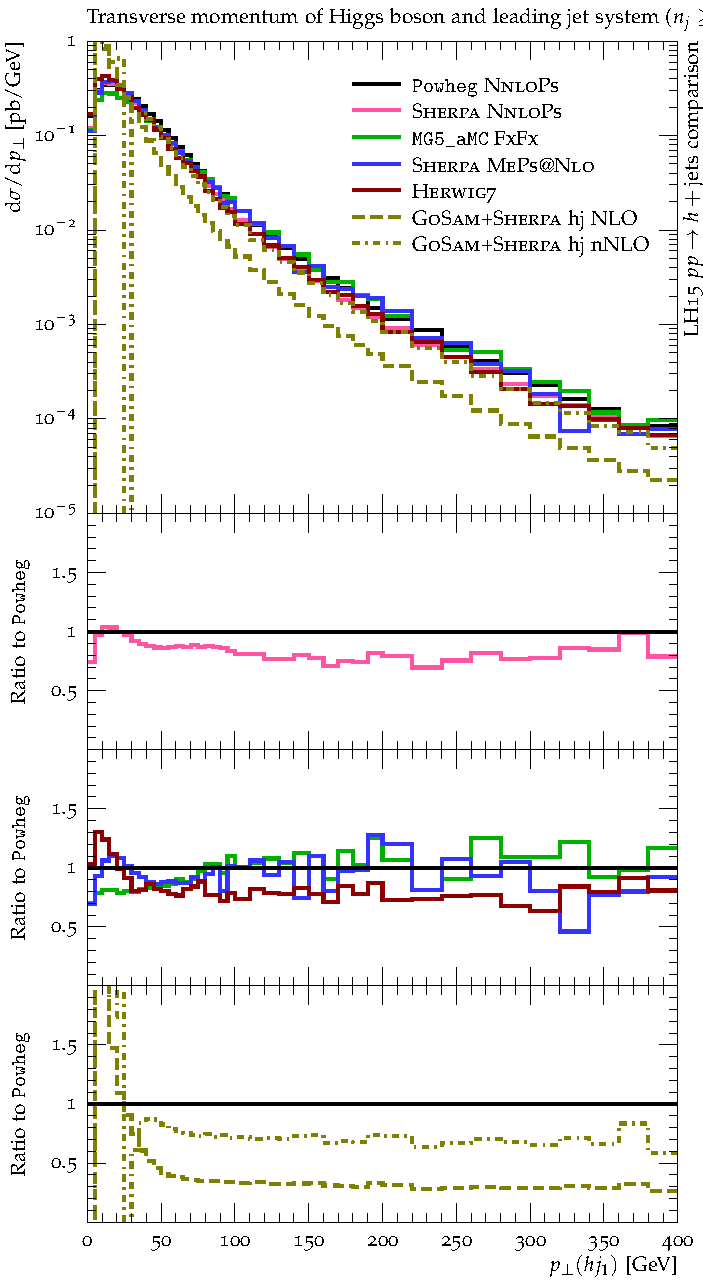
\includegraphics[width=0.47\textwidth]{figures/hjetscomp_u_Hj_pT_incl.pdf}
  \hfill
  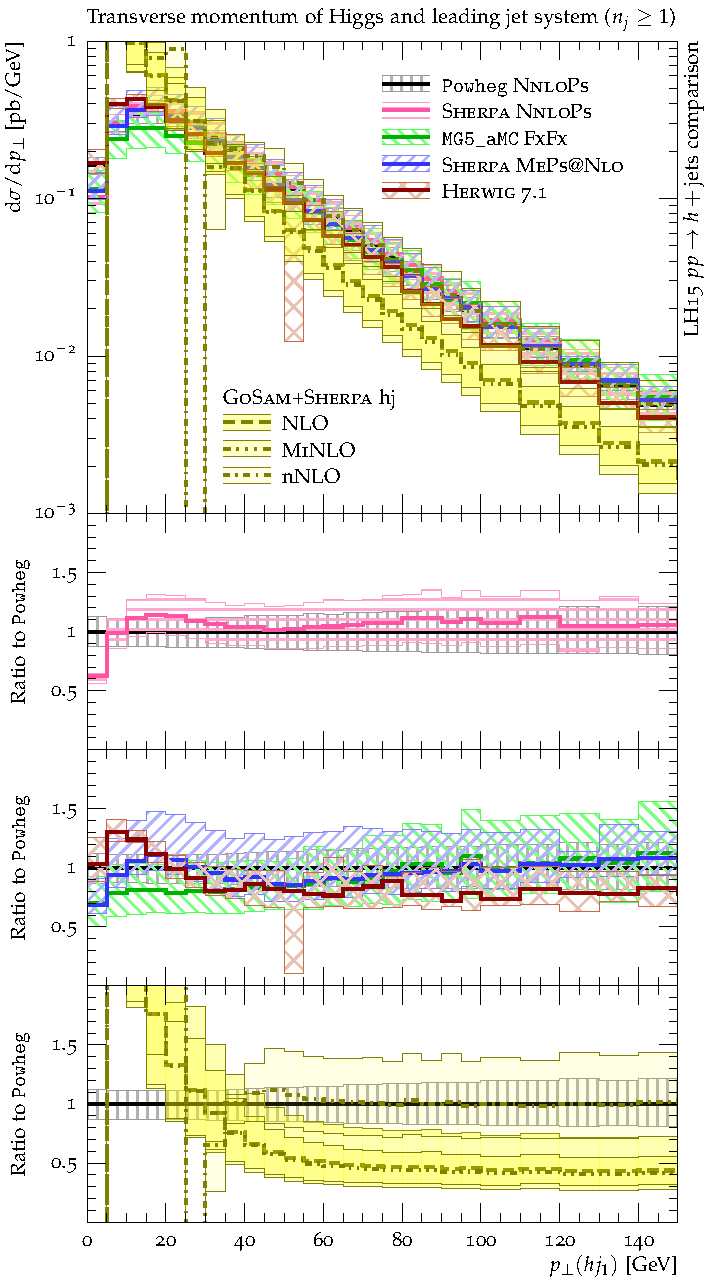
\includegraphics[width=0.47\textwidth]{figures/hjetscomp_Hj_pT_incl.pdf}
  \caption{\label{fig:hjetscomp:results:1obs:hj_pt}%
    The transverse momentum of the Higgs-boson-leading-jet system in
    the presence of at least one jet. For better visibility, results
    are shown without (left) and with (right) theoretical
    uncertainties. The plot layout exactly corresponds to that of
    Figure~\ref{fig:hjetscomp:results:1obs:j1y}, except for the
    extended $\hat y$-axis range in the ratio plots.}
\end{figure}

We finish this section by examining the results for the transverse
momentum of the Higgs-boson plus leading-jet system. In other words,
we are interested in studying the different descriptions of the
recoil of the $hj_1$ system. In the inclusive one-jet case depicted in
Figure~\ref{fig:hjetscomp:results:1obs:hj_pt}, the system may recoil
against a second jet (or secondary jets) plus soft radiation, while
for the exclusive jet scenario shown in
Figure~\ref{fig:hjetscomp:results:1obs:hj_pt_excl}, it is only soft
radiation that recoils against the $hj_1$ system. The latter case will
therefore be strongly affected by the level at which resummation is
taken into account. Formally, for the observable in question, the
predictions of highest accuracy are facilitated by the NLO merging
approaches as they provide an NLO description of the second jet; all
other predictions are only LO accurate in the second jet, i.e.~larger
differences can be expected. In the exclusive ($=1$-jet) case, all
predictions that include parton showering operate at the same level of
precision while the fixed-order calculations cannot do anything but
fail in describing the $p_\perp(hj_1)$ distribution.

For the $h\,+\!\ge\!1$-jet events, differences of $\mathcal{O}(30\%)$ are
observed among the ME+PS predictions below the jet threshold, while
there is better agreement at higher $p_\perp$ values, where again
\Herwig turns out to be on the softer side. The \Powheg and \Sherpa \NNLOPS 
curves surprisingly fit right in with the ME+PS results throughout 
the spectrum. The mostly comparable
behavior of the \NNLOPS results to those obtained from NLO merging is
not what one would expect a priori, however the NLO matching (\Powheg- 
and \SMCatNLO-type, respectively) of the $hj$ configurations transfers 
a differential $K$-factor to their second parton emission such that 
the LO+PS treatment of the $h\,+\!\ge\!2$-jet rate
obtains a more appropriate normalization. The $hj$ NLO calculations
(i.e.~the pure and \Minlo reweighted \GoSam{}+\Sherpa results) cannot
compete with this performance since they miss an adequate description 
of the second jet giving recoil to the $hj$ system.
Correspondingly, the $p_\perp(hj_1)$ observable is described poorly
with values clearly overshooting below the jet threshold due to the
missing Sudakov suppression and undershooting by 60\% beyond
$p_\perp=50\gev$ due to missing higher (than two-) jet multiplicity
contributions. It is interesting to see that the \Loopsim procedure
lifts this large discrepancy in the $p_\perp$ tail. This is evidence
that an adequate description of a second and third jet is sufficient
to describe this observable in this regime. Thus, the good agreement
with the ME+PS results is largely driven by the $hjj$ NLO component
used to build the nNLO prediction for the $h\,+\!\ge\!1$-jet
process. However, as a result of the cut-off dependence of the
procedure nothing can be said about the $p_\perp<25\gev$ region.
On the contrary, \Resbos predicts this region with NLL precision but
reverts to a LO description in the tail of the distribution leveling
off about 30\% above the \GoSam{}+\Sherpa result as a consequence of
employing a lower scale (that is $\mu=\tfrac{1}{2}m_h$). Note that for
the jet associated Higgs boson production, the transverse momentum of
the $hj_1$ system constitutes exactly the $q_\text{T}$ quantity that is to be
resummed by \Resbos imposing the constraint $p_\perp(hj_1)<p_\perp(j_1)$,
which is to ensure that $j_1$ is indeed the leading jet (as any other
jet is integrated out in the resummation formalism used by \Resbos).
In addition, terms of the form $\ln(1/R^2)$ are also taken into
account by the resummation carried out in \Resbos and lead to a
somewhat broader, upward shifted Sudakov peak.

\begin{figure}[t!]
  \centering
  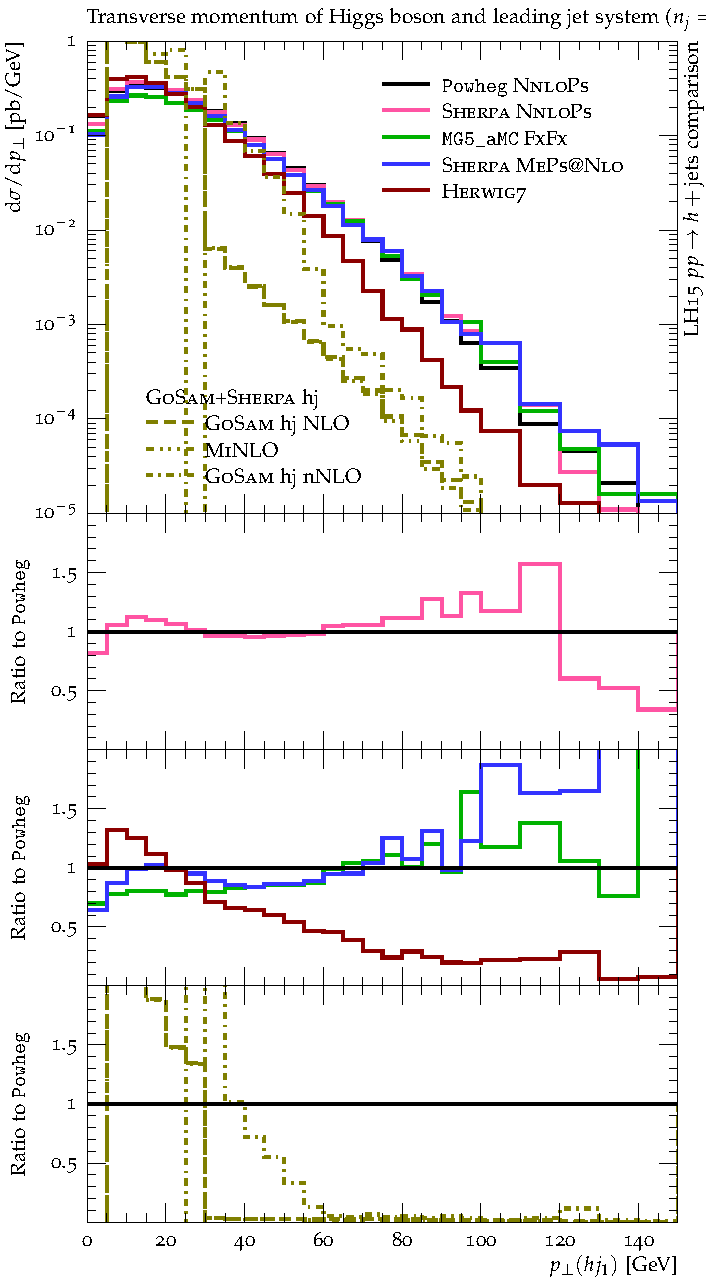
\includegraphics[width=0.47\textwidth]{figures/hjetscomp_u_Hj_pT_excl.pdf}
  \hfill
  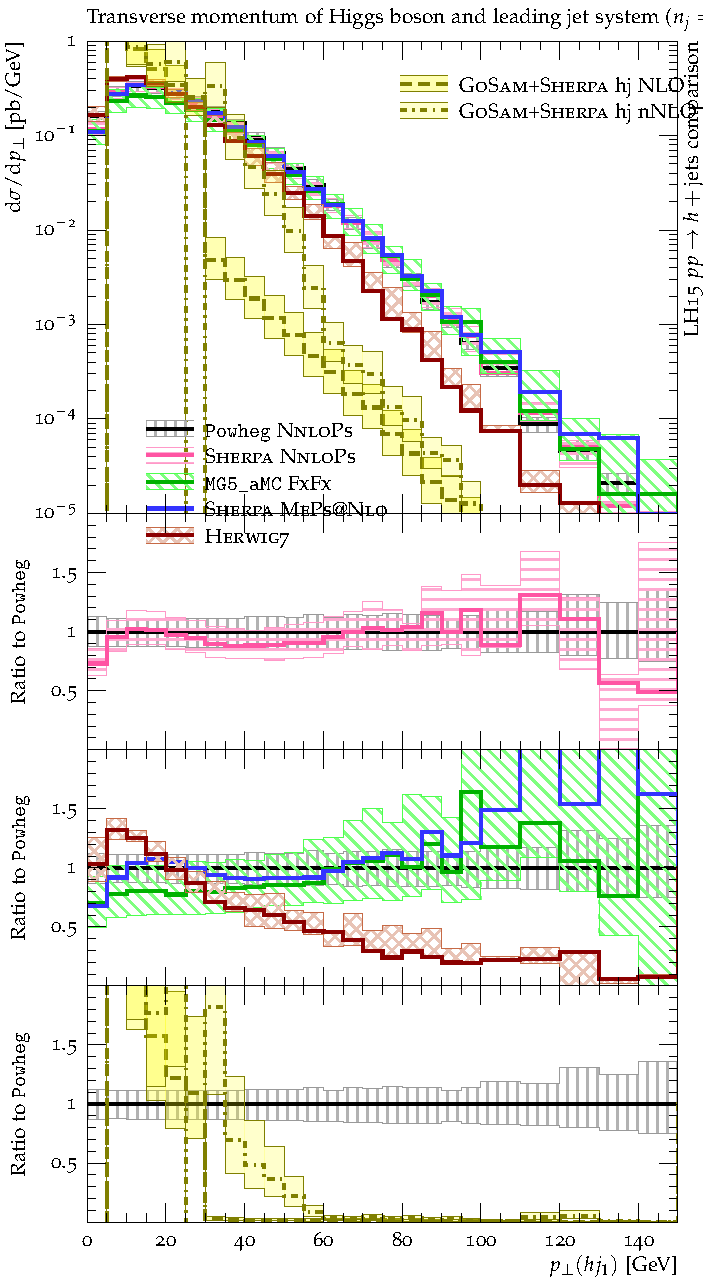
\includegraphics[width=0.47\textwidth]{figures/hjetscomp_Hj_pT_excl.pdf}
  \caption{\label{fig:hjetscomp:results:1obs:hj_pt_excl}%
    The transverse momentum of the Higgs-boson-leading-jet system in
    the presence of exactly one jet. Again, results are shown without
    (left) and with (right) theoretical uncertainties as given by the
    different groups. Note that the plot layout corresponds exactly to
    that of Figure~\ref{fig:hjetscomp:results:1obs:hpt_excl}, except
    for the extended $\hat y$-axis range used in the ratio plots.}
\end{figure}

Lastly, we comment on the uncertainties quoted by the different
calculations: the \Resbos, GoSam{}+\Sherpa NLO and \Minlo envelopes
have an appropriate size reflecting the underlying LO nature of the
$p_\perp(hj_1)$ prediction above the jet threshold. The \Loopsim
procedure leaves us with a somewhat wider band as it involves two
real-emission (LO-like) contributions ($hjj$ and $hjjj$), which impact
the $p_\perp(hj_1)$ observable.
\MGaMC and \Sherpa \MEPSatNLO on the one side and \Herwig on the other
side produce NLO variations that are fairly different in size.
However, the \Herwig as well as the \Powheg envelopes are most likely
underestimated; in particular the \Powheg band does not behave as
expected from a LO variation for above-jet-threshold $p_\perp$. The
\Sherpa \NNLOPS bands here are somewhat larger than those of \Powheg
but still do not reflect the LO nature of the prediction.

The exclusive (exactly one jet) case for the $p_\perp(hj_1)$
observable is shown in Figure~\ref{fig:hjetscomp:results:1obs:hj_pt_excl}.
Apart from the \NNLOPS outcomes, there is a much greater divergence of
the predictions for exactly one jet, especially at high $p_\perp$.
Recall that for this situation, the recoil is generated only from soft emissions, and
it is clear that a highly exclusive distribution such as the one in
question serves as a stress test for the ME+PS as well as the \NNLOPS
predictions (in fact any parton shower or resummed prediction). For
the same reason, caution has to be taken in interpreting the 
uncertainties. The current case is similar to the case for the Higgs
boson $p_\perp$ distribution with no jets and it is no surprise that
different approaches can lead to different answers. Most notably, we
observe \NNLOPS predictions that are in slightly worse agreement as
compared to the inclusive case, and the expected complete failure of the
\GoSam{}+\Sherpa results (including the \Loopsim result where the
one-jet requirement removes the effect that yielded the
improvement in the inclusive case),%
\footnote{Owing to the kinematic constraints on the jets, harder
  radiation that goes forward does not get identified as a jet;
  these contributions actually form the (naively unexpected)
  $p_\perp>30\gev$ tail of the \GoSam{}+\Sherpa results though the
  mechanism is highly suppressed.}
and the severe decline of the \Herwig differential cross section
dropping to about 25\% wrt.~the \Powheg result at $p_\perp\sim100\gev$.



\subsubsection{Dijet observables}
\label{sec:hjetscomp:results:2jobs}

\begin{figure}[t!]
  \centering
  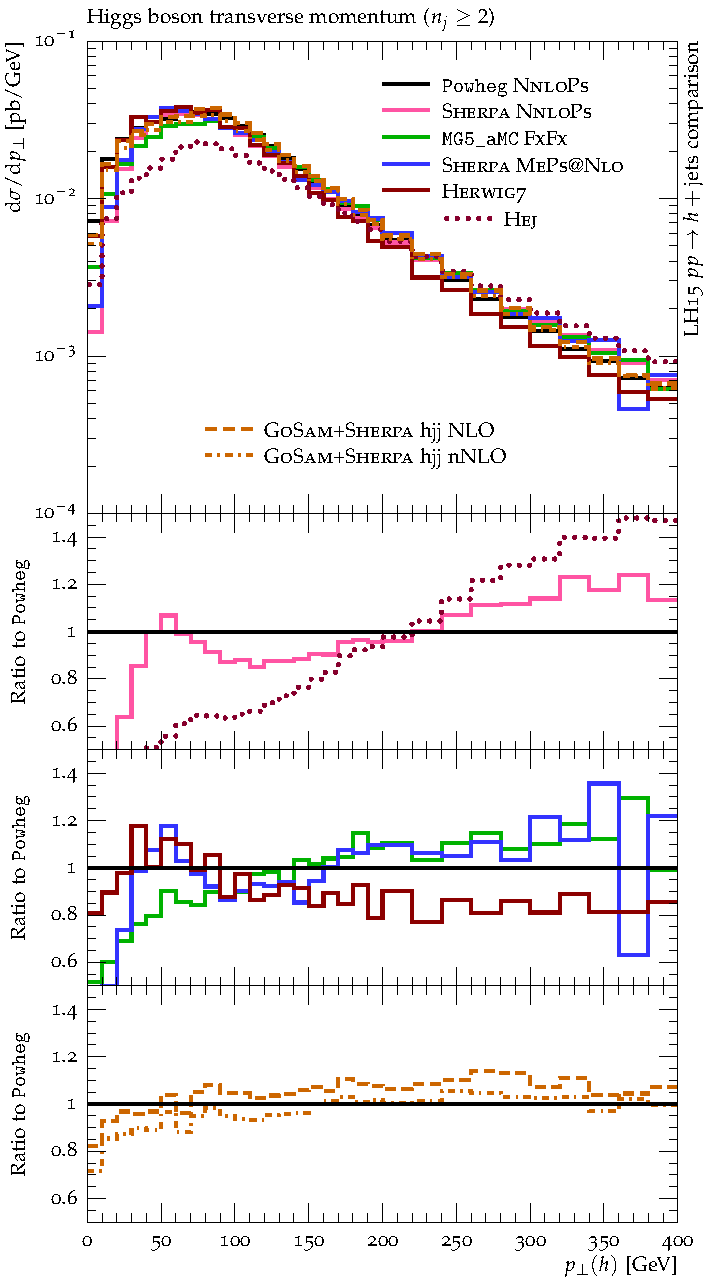
\includegraphics[width=0.47\textwidth]{figures/hjetscomp_u_H_jj_pT_incl.pdf}
  \hfill
  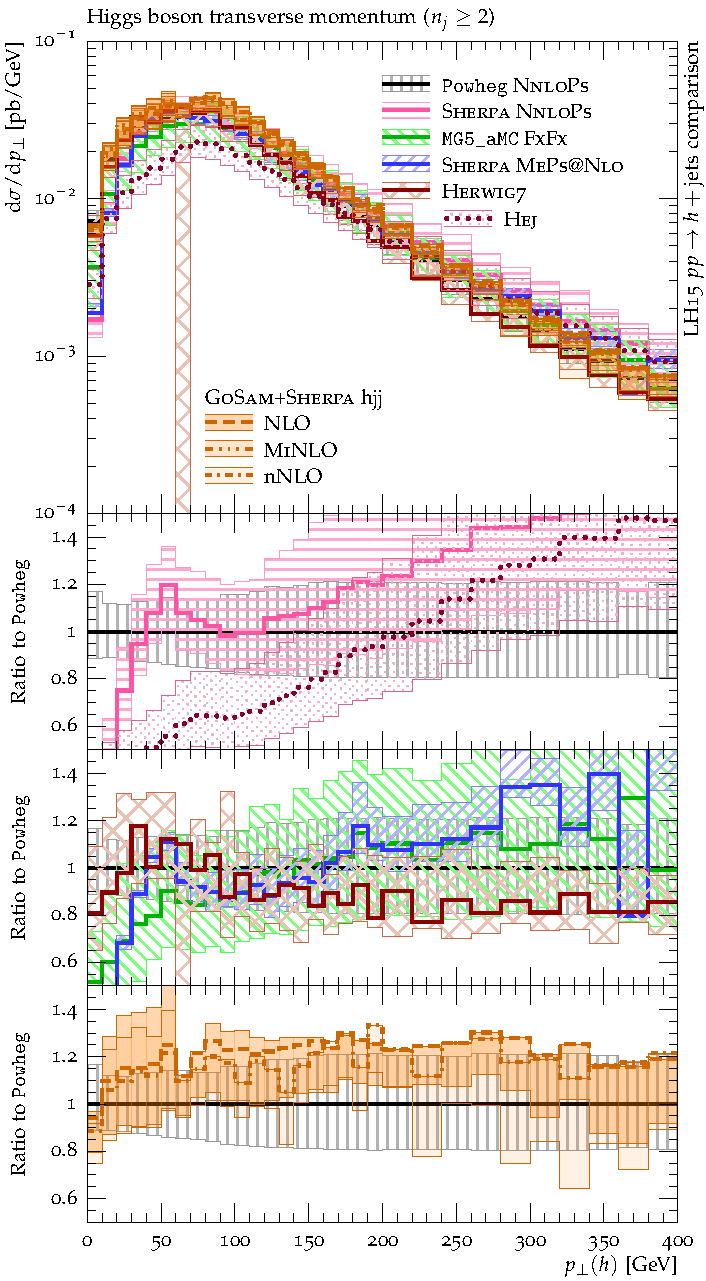
\includegraphics[width=0.47\textwidth]{figures/hjetscomp_H_jj_pT_incl.pdf}
  \caption{\label{fig:hjetscomp:results:2obs:hpt}%
    The transverse momentum of the Higgs boson in the presence of at
    least two jets without (left) and with (right) uncertainties,
    supplemented by three ratio plots using the reference result as
    obtained from \Powheg's \NNLOPS calculation for $h$ production.
    The predictions are grouped -- from top to bottom -- according to
    the categories \NNLOPS $h$ production, ME+PS merging at NLO (at
    least up to two jets) and NLO fixed-order $hjj$ production. \Hej's
    prediction is added to the first, the \NNLOPS subpanel.}
\end{figure}

Moving to topologies with one more jet in the final state, 
we discuss a number of $h+2$-jet
observables in this section. Following the previous sections, we compare predictions from three
different categories with each other: \NNLOPS $h$ production,
\MEPSatNLO $h+\text{jets}$ production and fixed-order (and related)
$hjj$ production at $\mathcal{O}(\alpha_\mathrm{s}^5)$. It is important
to understand, in detail, the level of (dis-)agreement among the
available predictions since the $h+2$-jet gluon fusion contribution
constitutes the major irreducible background in any LHC Run-II analysis
targeting the prominent vector boson fusion channel. As before we have
provided one ratio plot for each category in order to enhance the
readability of our plots; common to all figures is the use of \Powheg's
\NNLOPS prediction to serve as the reference result. Note that for
each category, the accuracy with which the $h+2$-jet events are
described is different: the \NNLOPS predictions are at the LO+PS level
while the multijet merged results incorporate the precision given by NLO+PS
matching. \Hej generates predictions derived from the behavior of QCD
in the high-energy limit, starting from a LO accurate $h+2$-jet configuration.
With two or more jets in the final state,
\Hej can provide meaningful predictions for the first time. As
for earlier cases, the last category contains NLO-accurate predictions
solely, free of any parton showering.

\begin{figure}[t!]
  \centering
  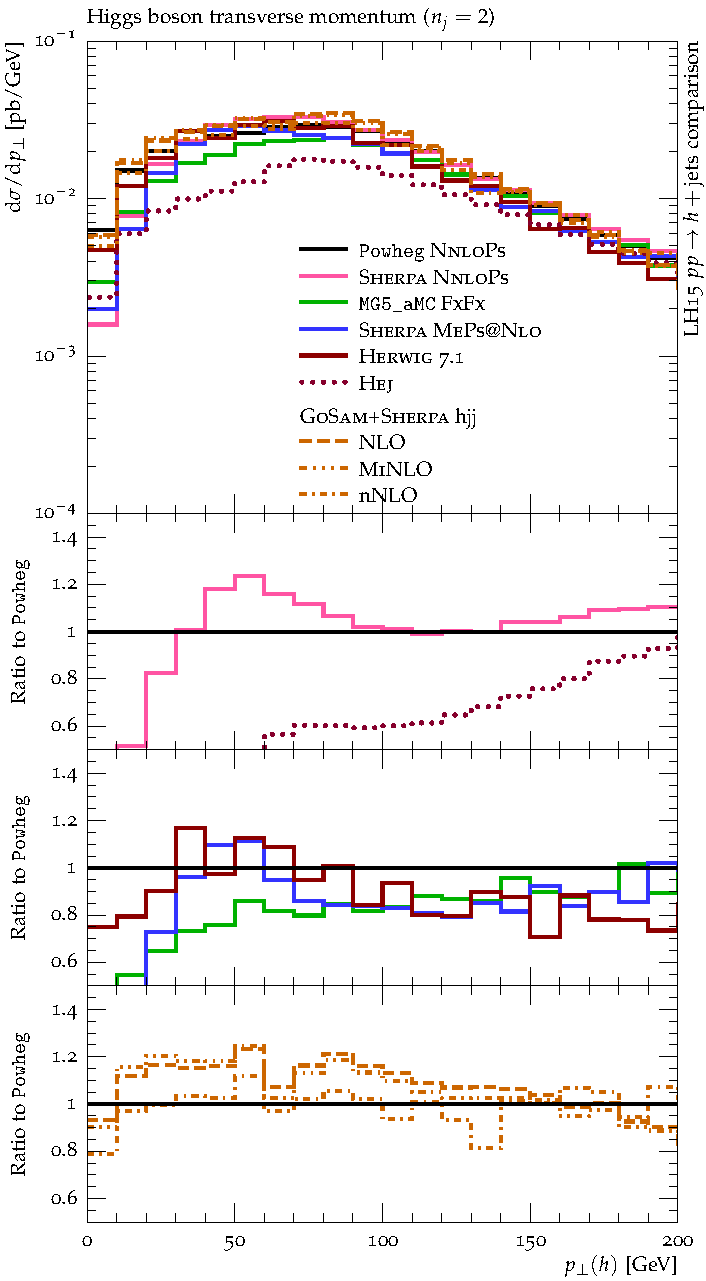
\includegraphics[width=0.47\textwidth]{figures/hjetscomp_u_H_jj_pT_excl.pdf}
  \hfill
  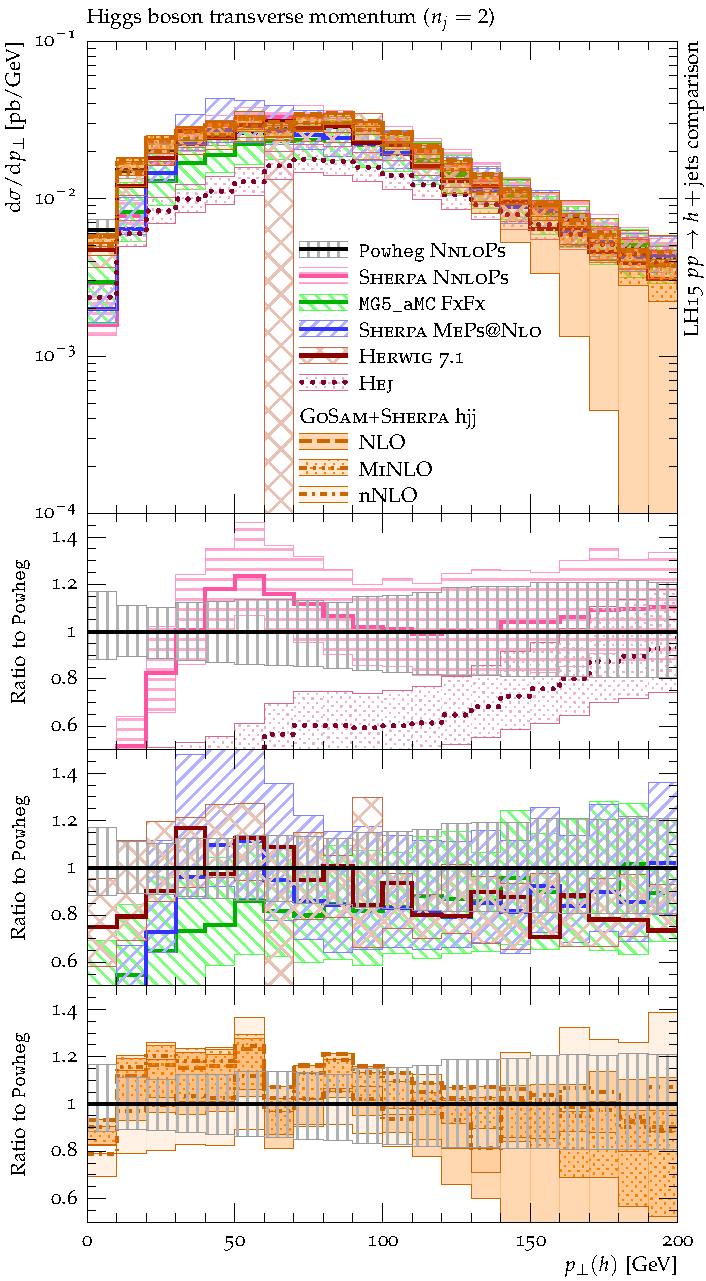
\includegraphics[width=0.47\textwidth]{figures/hjetscomp_H_jj_pT_excl.pdf}
  \caption{\label{fig:hjetscomp:results:2obs:hpt_excl}%
    The transverse momentum of the Higgs boson in the presence of 
    exactly two jets without (left) and with (right) uncertainties,
    supplemented by three ratio plots using the reference result as
    obtained from \Powheg's \NNLOPS calculation for $h$ production.
    The predictions are grouped -- from top to bottom -- according to
    the categories \NNLOPS $h$ production, ME+PS merging at NLO (at
    least up to two jets) and NLO fixed-order $hjj$ production. \Hej's
    prediction is added to the first, the \NNLOPS subpanel.}
\end{figure}

The Higgs boson $p_\perp$ spectrum, in the presence of at least two
jets, is shown in Figure~\ref{fig:hjetscomp:results:2obs:hpt}.
Here, although all calculations agree on the position of the maximum
of the distribution (situated at $p_\perp\gtrsim 60\gev$, i.e.~twice the 
jet threshold),\footnote{Note that around this two-jet threshold, we
  again find remnants of the Sudakov shoulder effect affecting the
  fixed-order predictions.}
varying behavior is observed for both larger and smaller 
transverse momenta. Examining first the region where $p_\perp\gtrsim 
60\gev$, good agreement between all multijet merged calculations and 
\Powheg is found. Only \Herwig predicts a somewhat more rapidly falling 
distribution. \Sherpa \NNLOPS, due to its scale choice, exhibits a 
more or less constant $\mathcal{O}(+20\%)$ offset with respect to the
\Powheg \NNLOPS, but remains well within their respective uncertainties.
In comparison to all the NLO uncertainty bands, the \NNLOPS envelopes
are expected to be larger reflecting the loss of one order in accuracy.
A clear difference however is not found indicating that the \NNLOPS
estimates are too optimistic. From this point of view, the larger
difference seen between the two \NNLOPS predictions is no surprise at
all -- rather typical for comparisons at the LO+PS level, and two
fairly different parton showers at work. The fixed-order
predictions (NLO, \Minlo and \Loopsim) agree well in this region with
one another, but surpass the \Powheg reference and, more importantly,
the multijet merged calculations with the same accuracy, by about 
20\%. This deviation is just covered by the edge of the uncertainty
bands associated with either of the NLO calculations. Finally, \Hej
clearly produces the hardest spectrum in this region, exhibiting a
considerably different slope with respect to all other calculations,
albeit it starts out from an approximately 40\% lower cross section at
$p_\perp\approx 60\gev$.

In the region below the peak, $p_\perp\lesssim 60\gev$, the various
calculations are more widely spread. This is expected as effects from
parton showering have a larger impact here, but none of the considered
shower Monte Carlos in Figure~\ref{fig:hjetscomp:results:2obs:hpt}
works at a higher level regarding the resummation precision. We can
readily distinguish between two topologies if we assume the jets to be
produced near their $p_\perp$ threshold: while for
$p_\perp(h)>30\gev$, both the leading and subleading jet have to be in
the same hemisphere opposite the Higgs boson, for
$p_\perp(h)<30\gev$, the subleading jet has to cross over into the
Higgs boson's hemisphere opposite the leading jet.
Because of  parton shower effects, deviations among the predictions
are greater in the former region, but it is the latter region that
receives the larger resummation corrections, as both jets recoil mainly
against each other (to form a jet-balanced configuration) and soft
radiation off them has a large influence on the small Higgs boson
transverse momentum. An important role is also played by the
assignment of scales in the context of multijet merging.
To assign a meaningful history in this regime, in particular
for sufficiently hard jets, the clustering algorithm that is needed to
define the local CKKW or \Minlo scales must allow for the possibility
of Higgs boson radiation off a dijet process. In consequence, the value
of the scales increases and the cross section is reduced, explaining
the identical behavior of both the \Sherpa \MEPSatNLO and \Sherpa
\NNLOPS predictions.
The \Herwig, \MGaMC and \Hej predictions are largely similar in shape,
but offset as a result of the larger central scale choice in \MGaMC
and the LO accuracy of the total cross section in \Hej. \Powheg
\NNLOPS gives the slowest decline of the differential cross section as
$p_\perp\to0$.
The various fixed-order predictions are somewhat more widely spread than
for large $p_\perp$ (as indicated by the wider uncertainty bands), and
start to exhibit a slope wrt.~the \Powheg reference, retaining however
a more or less constant ratio wrt.~\Herwig and \MGaMC. In the
$p_\perp(h)$ region below $30\gev$, the global scale setting of the
fixed-order calculations is certainly not flexible enough to deal with
the jet-balanced configurations in a similar way as done by \Sherpa.

Figure \ref{fig:hjetscomp:results:2obs:hpt_excl} displays the 
Higgs boson's transverse momentum in the presence of exactly two jets. 
Apart from the overall reduction of the cross section, the general 
features as observed in Figure~\ref{fig:hjetscomp:results:2obs:hpt}
for each generator are reproduced. There are, however, two notable
exceptions. The decrease in the \Powheg \NNLOPS prediction at large $p_\perp(h)$ 
is less, as compared to
the other generators. On the one hand, it now overshoots the multijet
merged predictions by about 10-20\%, but on the other hand it achieves
a much better agreement with \Sherpa \NNLOPS. This, however, is not
very surprising given that the jet veto (on the third jet) in the
\NNLOPS calculations is only described at parton shower level, lacking
any matrix element input. The latter is mandatory for a good
description of the rejected $30\gev$ emission. As seen before, the
fixed-order predictions start to lose their perturbative stability when
the $p_\perp$ ratio between the observed Higgs boson and the rejected
jet turns out to be large. This effect is more pronounced for the
\Minlo procedure because it generates lower scale values on
average. In the \Loopsim approach, perturbative stability is
improved as a result of the inclusion of $hjjj$ information.

\begin{figure}[t!]
  \centering
  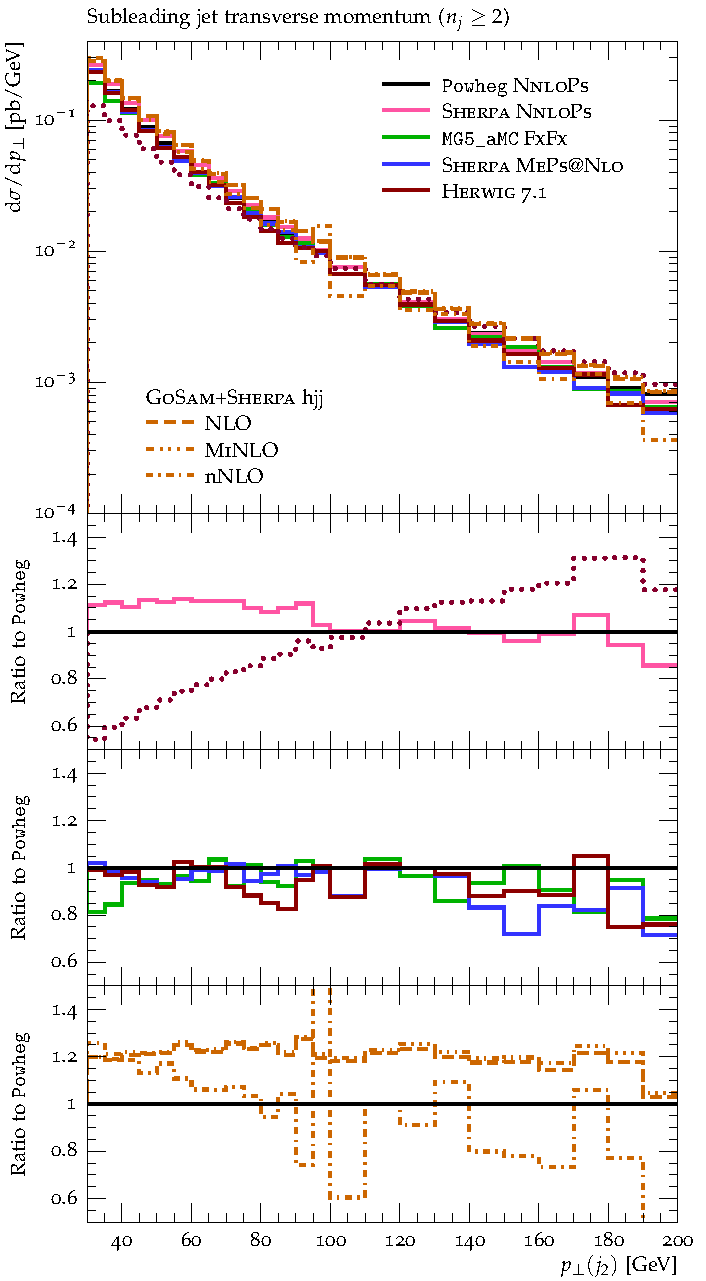
\includegraphics[width=0.47\textwidth]{figures/hjetscomp_u_jet2_pT_incl.pdf}
  \hfill
  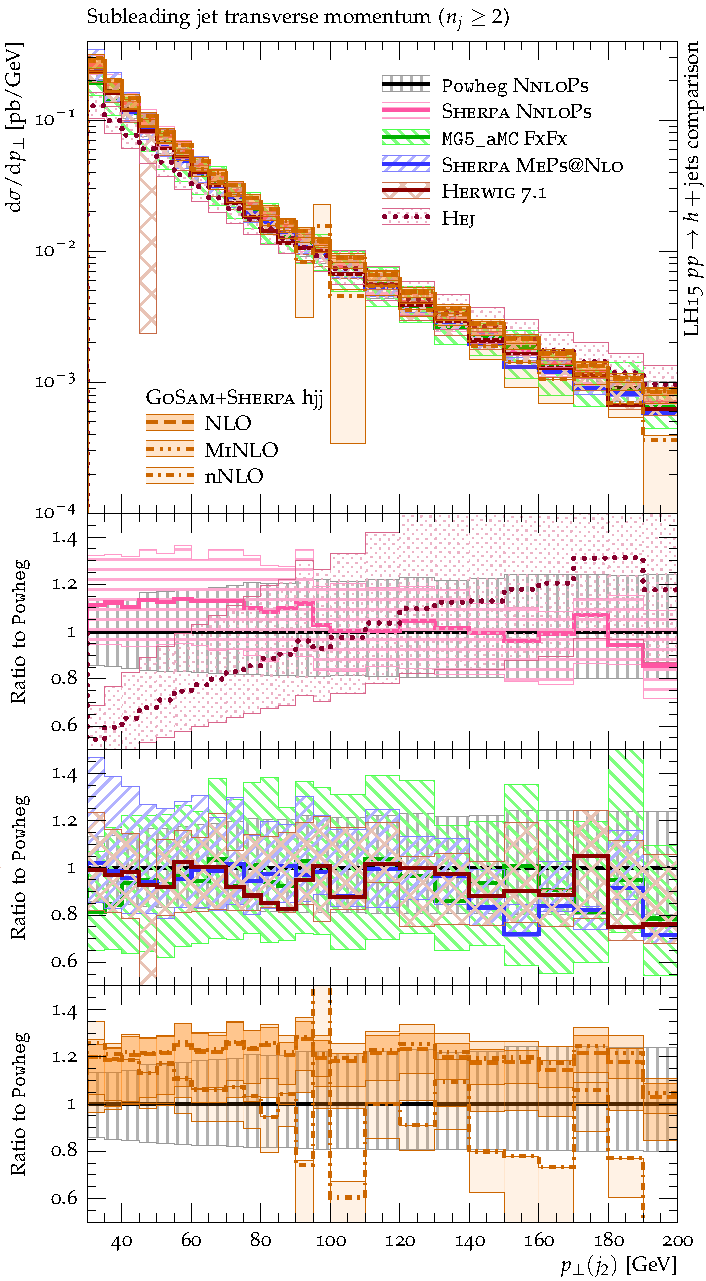
\includegraphics[width=0.47\textwidth]{figures/hjetscomp_jet2_pT_incl.pdf}
  \caption{\label{fig:hjetscomp:results:2obs:jet2_pt}%
    The subleading jet $p_\perp$ for $h\,+\!\ge\!2$-jets production shown
    without (left) and with (right) theoretical uncertainties. The
    plot layout is the same as in the previous figure.}
\end{figure}

\begin{figure}[t!]
  \centering
  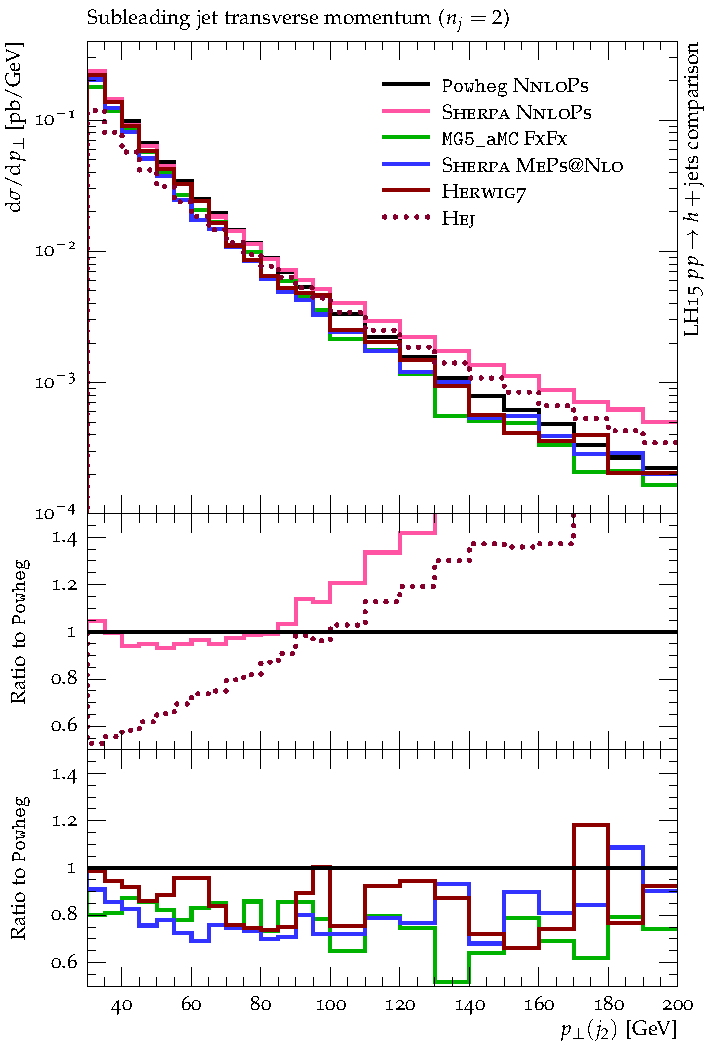
\includegraphics[width=0.47\textwidth]{figures/hjetscomp_u_jet2_pT_excl.pdf}
  \hfill
  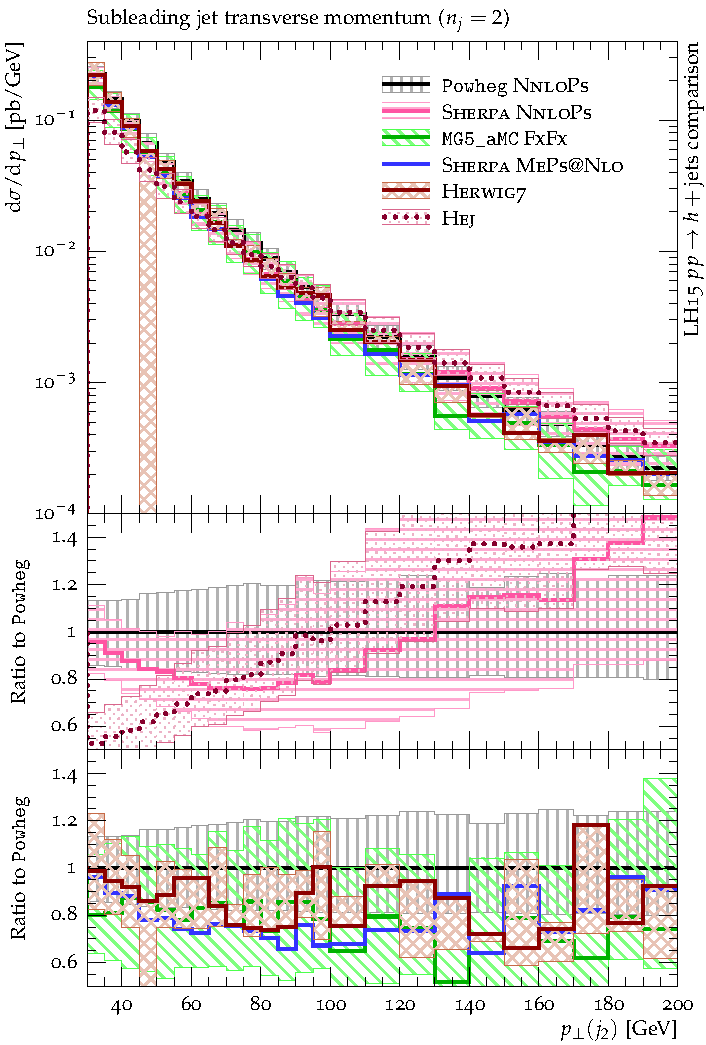
\includegraphics[width=0.47\textwidth]{figures/hjetscomp_jet2_pT_excl.pdf}
  \caption{\label{fig:hjetscomp:results:2obs:jet2_pt_excl}%
    The subleading jet $p_\perp$ for exclusive $h+2$-jets production
    shown without (left) and with (right) theoretical uncertainties.
    Again, the layout is similar to that of
    Figure~\ref{fig:hjetscomp:results:2obs:hpt} except for
    dropping the results of the NLO fixed-order $hjj$ production and
    the associated ratio subpanel.}
\end{figure}

The subleading jet $p_\perp$ spectra for $h+\ge2$ and $h$ plus exactly
two jets are shown in Figures~\ref{fig:hjetscomp:results:2obs:jet2_pt}
and \ref{fig:hjetscomp:results:2obs:jet2_pt_excl}, respectively. A
comparison between the second jet results (of the
$n_j\ge2$ and $n_j=2$ case) with the first jet results (of the
$n_j\ge1$ and $n_j=1$ case, depicted in
Figures~\ref{fig:hjetscomp:results:1obs:j1pt} and
\ref{fig:hjetscomp:results:1obs:j1pt_excl}, respectively) reveals a
rather consistent picture. The agreement among the ME+PS
predictions, and between the ME+PS and the \Powheg predictions, is
slightly better than in the case of the leading jet. For $n_j=2$
(cf.~Figure~\ref{fig:hjetscomp:results:2obs:jet2_pt_excl}), \Powheg's
\NNLOPS approach predicts harder subleading jets than the others do,
apart from \Hej. \MGaMC, \Sherpa and \Herwig lie in reasonable
agreement with each other, but systematically lower than \Powheg by
about 10-20\%. The agreement in the inclusive (i.e.~$n_j\ge2$) case
eventually results from a compensating effect, since all the different
methods for NLO merging give larger three-jet rates wrt.~\Powheg. The
\GoSam{}+\Sherpa $hjj$ NLO predictions do not have a different shape,
but their rate is higher, which likely comes from choosing
$\tfrac{1}{2}\sum_T^{1/2}$ as the central scale; recall that in the
one-jet case this choice already produced large NLO cross sections, as
large as the NNLO one, and larger than the ME+PS ones. With two jets
in the final state, this effect is easily seen to be enhanced. The
\Loopsim NNLO estimate for the $p_\perp(j_2)$ spectrum gradually
decreases wrt.~the other \GoSam results, in a similar, slightly more
pronounced way to what we found for $p_\perp(j_1)$ in the $n_j\ge1$
case. 
\Loopsim combines the NLO-accurate $hjj$ and $hjjj$ bins, and in doing
so  seems closer to the NLO-merged results, and therefore reproduces
some of their characteristics. The hardest spectrum is
delivered by \Hej even though its total rate is significantly lower. 
In the plot range, \Hej's prediction is consistent with the others due 
to overlapping uncertainties (LO for \Hej), but this statement gets
stretched for the exclusive two-jet scenario. Moreover, for $n_j=2$,
the   uncertainties reported here have to be considered with caution,
owing to the neglect of important resummation effects. However, the
statements made regarding error estimates when discussing 
$p_\perp(h)$ for $n_j\ge2$, carry over to the current case, as well as
for all other observables in this section.

\begin{figure}[t!]
  \centering
  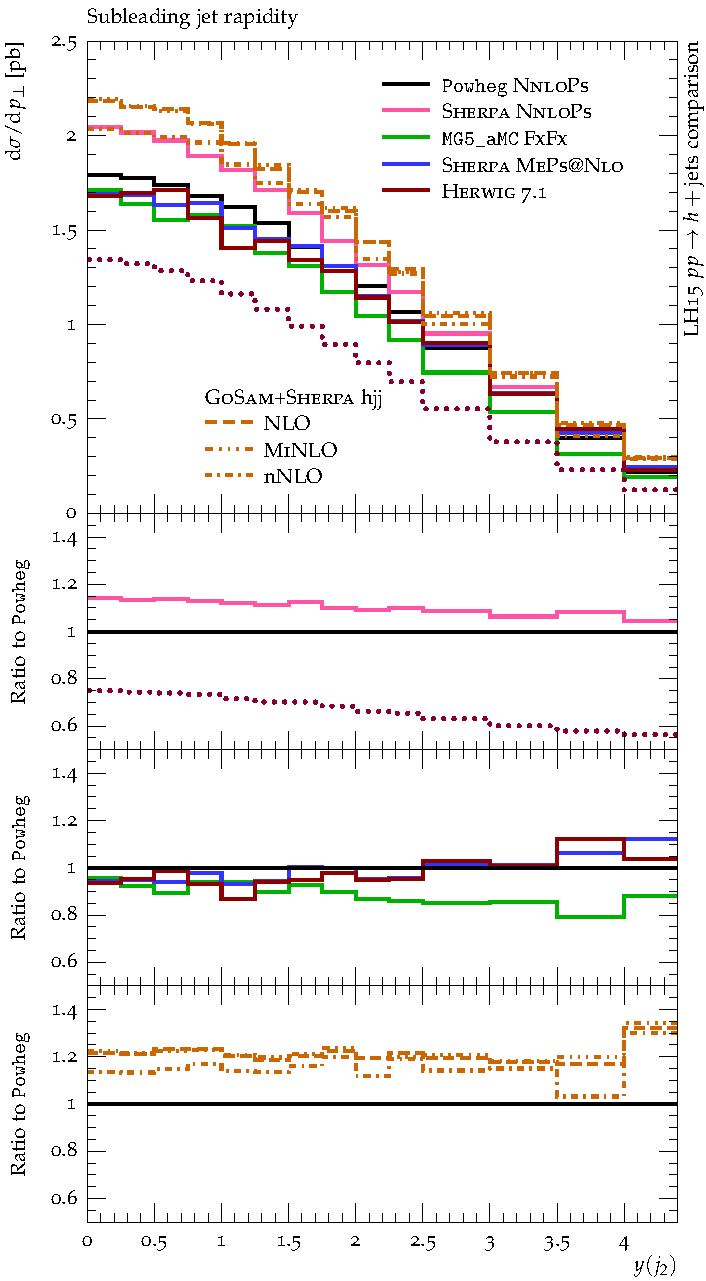
\includegraphics[width=0.47\textwidth]{figures/hjetscomp_u_jet2_y.pdf}
  \hfill
  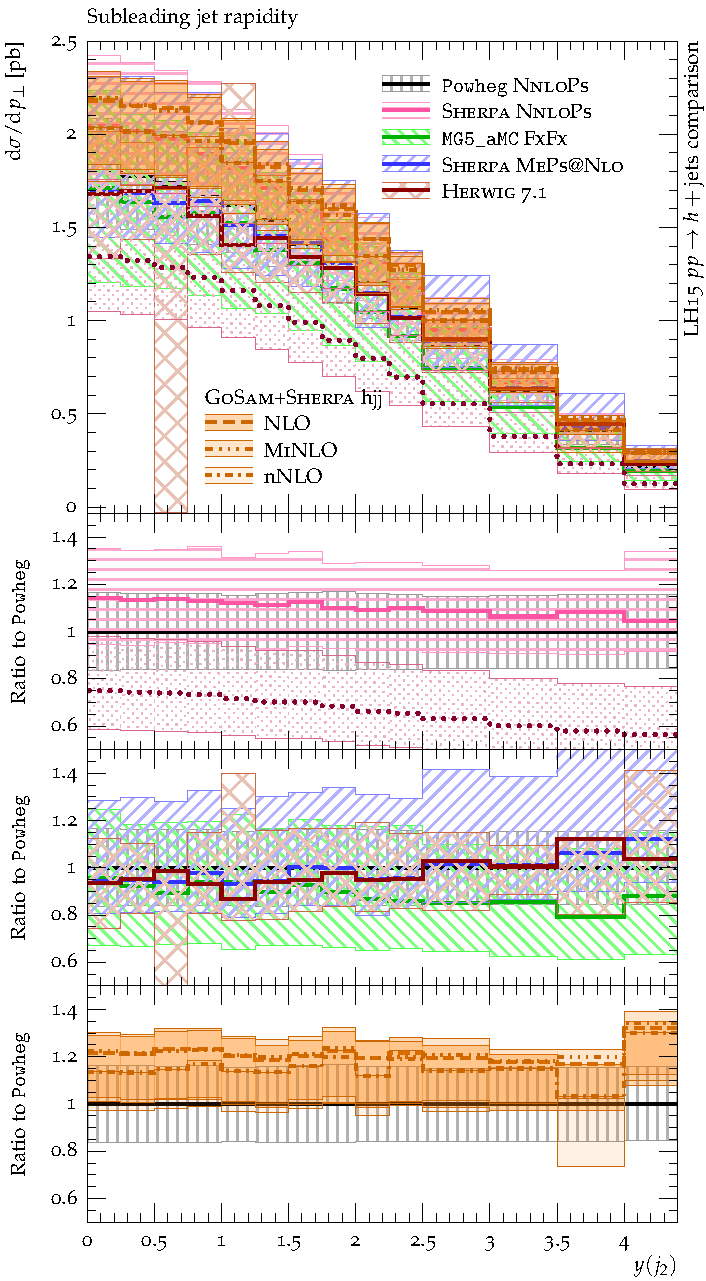
\includegraphics[width=0.47\textwidth]{figures/hjetscomp_jet2_y.pdf}
  \caption{\label{fig:hjetscomp:results:2obs:j2y}%
    The rapidity separation between the leading and subleading jets
    for $h\,+\!\ge\!2$-jets production, shown without (left) and with
    (right) theoretical uncertainties. The plot layout is the same as
    the one used in Figure~\ref{fig:hjetscomp:results:2obs:hpt}.}
\end{figure}

Figure~\ref{fig:hjetscomp:results:2obs:j2y} depicts the rapidity
distribution of the subleading jet. The conclusion of this comparison is
more or less the same as for the leading jet, see
Figure~\ref{fig:hjetscomp:results:1obs:j1y}. Only minor differences 
between the computations are encountered, in particular concerning the
shape of the rapidity spectrum -- the larger effects are driven by the
different rate predictions. While \Sherpa \NNLOPS and \MGaMC prefer a
slightly more central production than the other calculations, the
 rate difference previously observed between \Powheg \NNLOPS, \MGaMC,
\Herwig and \Sherpa \MEPSatNLO on the one side, and \Sherpa \NNLOPS and
the various \GoSam{}+\Sherpa NLO calculations on the other side, is the
feature that most stands out when plotting the subleading jet rapidity.
The largest deviations are again delivered by \Hej; apart from the
lower total rate, \Hej predicts fewer subleading jets at large
rapidities than the other approaches. It again becomes apparent that
the quoted uncertainties of the \NNLOPS calculations are likely
underestimated.

\begin{figure}[t!]
  \centering
  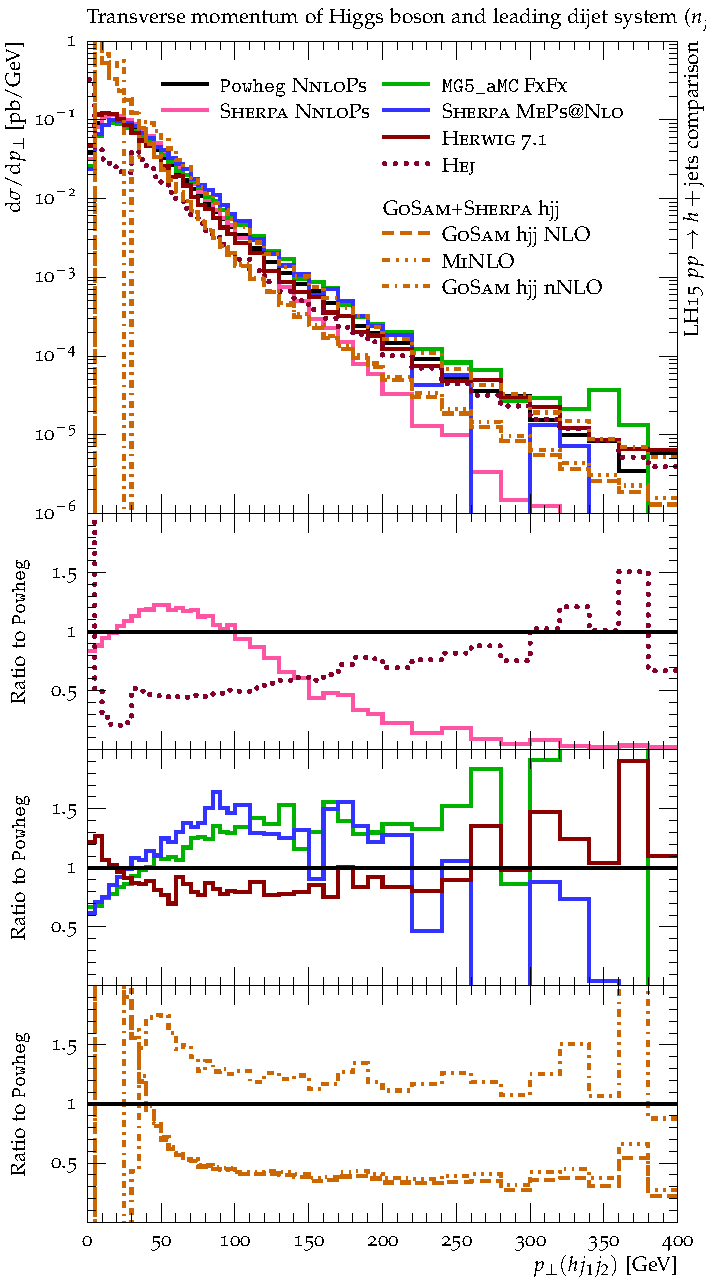
\includegraphics[width=0.47\textwidth]{figures/hjetscomp_u_Hjj_pT_incl.pdf}
  \hfill
  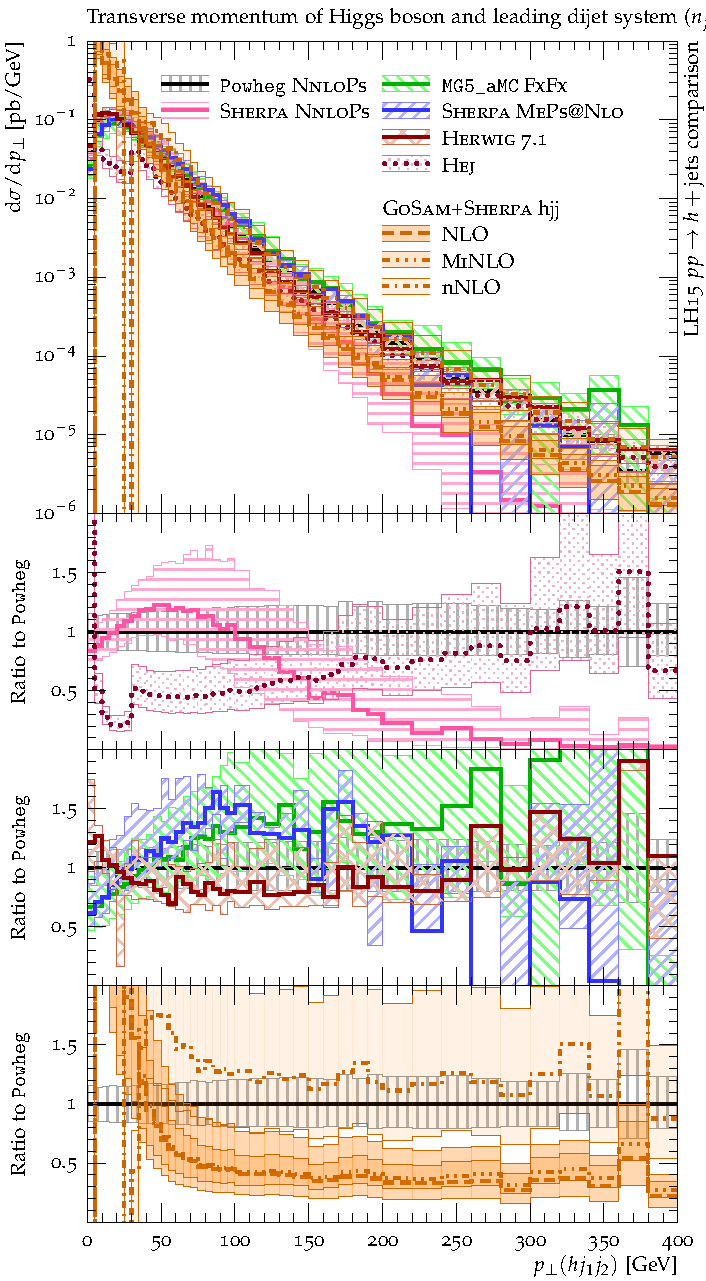
\includegraphics[width=0.47\textwidth]{figures/hjetscomp_Hjj_pT_incl.pdf}
  \caption{\label{fig:hjetscomp:results:2obs:hjj_pt}%
    The transverse momentum distribution of the Higgs boson plus two
    leading jet system, shown without (left) and with (right)
    uncertainties. The plot layout is the same as in
    Figure~\ref{fig:hjetscomp:results:2obs:hpt}.}
\end{figure}

As before, we are also interested in multiparticle or system
observables. As an example we show the transverse momentum
distribution of the Higgs boson plus two leading jet system in
Figure~\ref{fig:hjetscomp:results:2obs:hjj_pt}. The $p_\perp(hj_1j_2)$
variable is the two-jet analog of the $p_\perp(hj_1)$ variable for
inclusive one-jet events. The physics of this type of recoil
observable has been already discussed in detail around
Figure~\ref{fig:hjetscomp:results:1obs:hj_pt}, and simply applies to
the current case as well. The variations between the different
approaches are similar to the $p_\perp(hj_1)$ case of
Figure~\ref{fig:hjetscomp:results:1obs:hj_pt}, but turn out
to be somewhat stronger. \MGaMC and \Sherpa have a slope with respect
to \Powheg at low $p_\perp$ and overshoot by about 25\% at higher
$p_\perp$, while \Herwig is again somewhat lower than \Powheg at high
$p_\perp$. In the soft domain, the \Sherpa \NNLOPS result resembles
the corresponding ME+PS one as a result of using the same parton
shower. While the latter prediction levels off above \Powheg (due to
the ME description of a third jet at NLO), the former falls back to
the same level slightly above the plotted range. Recall that for 
\Sherpa \NNLOPS a third, fourth and so
forth jet is described by the parton shower only, the same as for \Powheg.
The behavior of \Hej is again largely affected by the lower rate. The
shape difference once more puts emphasis on the fact that \Hej
generates harder transverse momentum spectra in general while possessing 
a discontinuity where the events start to possess a resolved third jet. 
In the \GoSam{}+\Sherpa NLO predictions, the recoil is solely
described by the real emission contribution, hence the divergent
behavior in the soft domain and the significantly lower rate but
constant LO shape wrt.~\Powheg at higher $p_\perp$. For the same
reason, the associated uncertainty bands are found to be larger as
well. \Loopsim, as before, benefits from the fact that the third
jet enters at NLO accuracy, but cannot describe the soft region due to
the procedure's cut-off dependence. Also, \Loopsim's uncertainty band
is relatively wide due to the strong impact of the four-jet
contributions on the $p_\perp(hj_1j_2)$ distribution. On the positive
side, these contributions are only included because of \Loopsim's
combination of jet bins, while on the negative side they are described
with  LO accuracy. Note that this peculiar behavior of the
$p_\perp(hj_1j_2)$ observable has been already pointed out and
discussed in more detail in Ref.~\cite{Greiner:2015jha}.

\begin{figure}[t!]
  \centering
  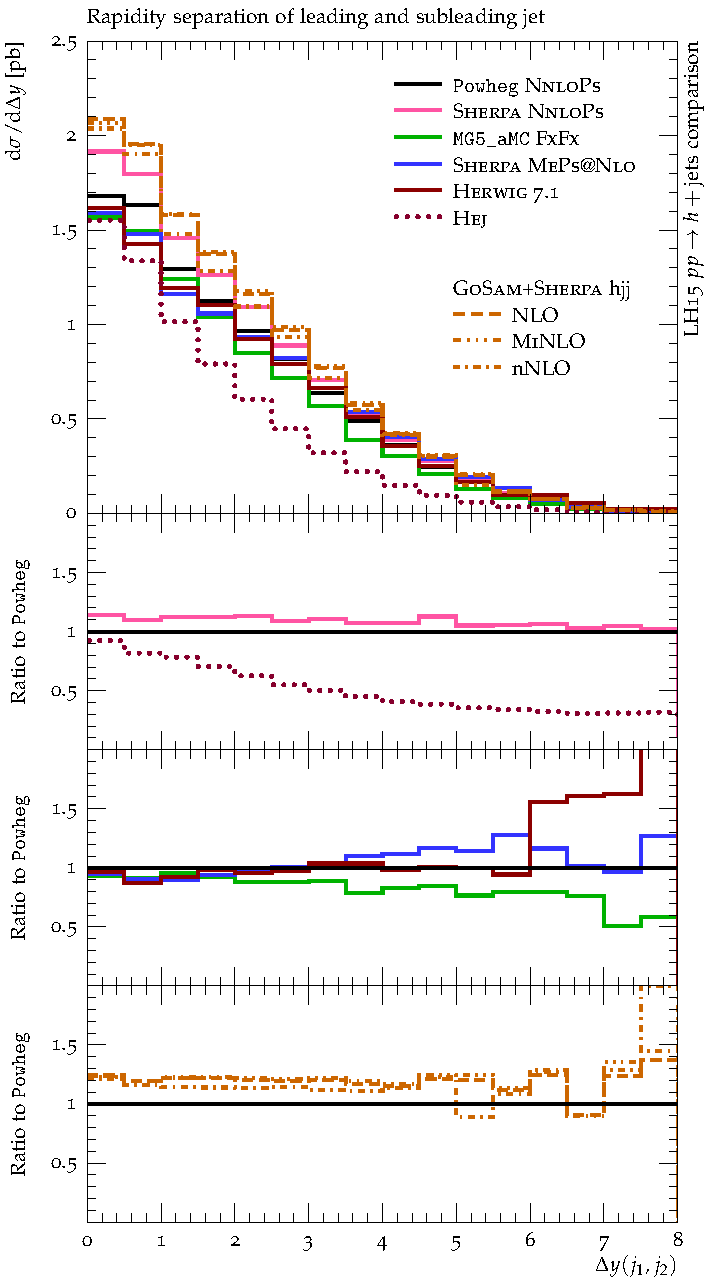
\includegraphics[width=0.47\textwidth]{figures/hjetscomp_u_deltay_jj.pdf}
  \hfill
  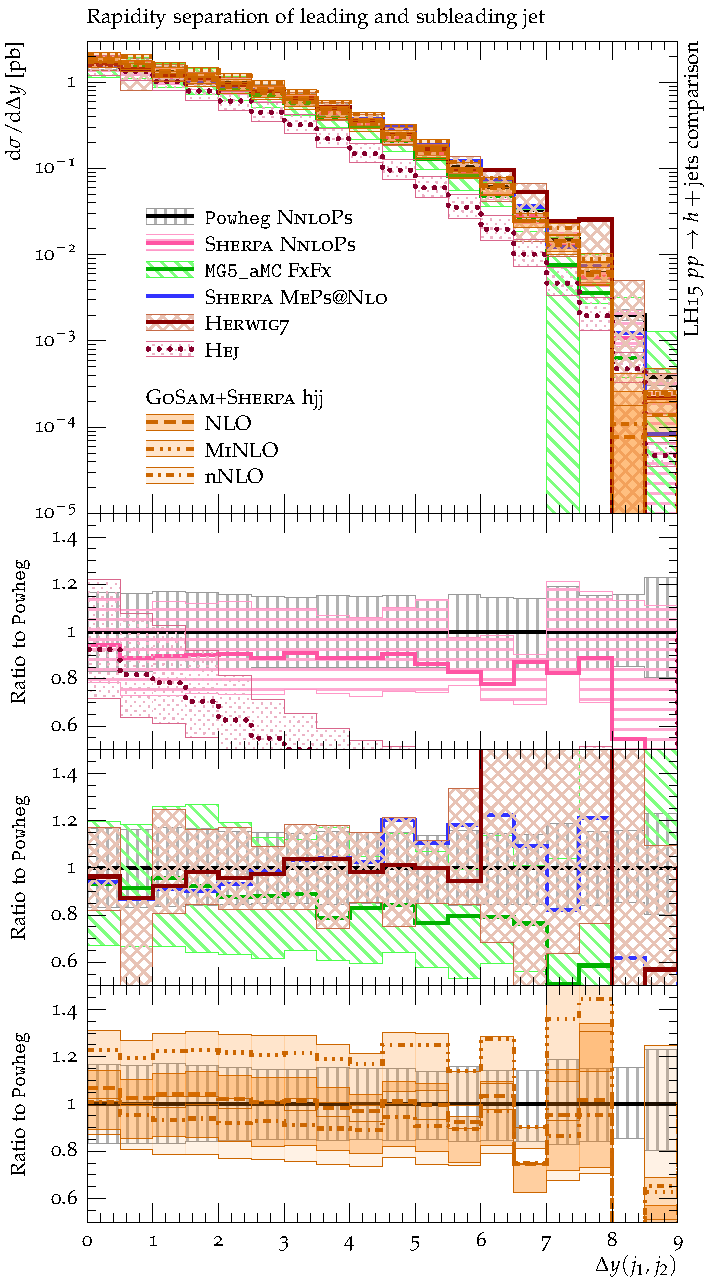
\includegraphics[width=0.47\textwidth]{figures/hjetscomp_deltay_jj.pdf}
  \caption{\label{fig:hjetscomp:results:2obs:dyjj}%
    The rapidity separation between the leading and subleading jets
    for $h\,+\!\ge\!2$-jets production, shown without (left) and with
    (right) theoretical uncertainties. The plot layout is the same as
    the one used in Figure~\ref{fig:hjetscomp:results:2obs:hpt}.}
\end{figure}

We now turn to the discussion of jet--jet correlations.
The rapidity separation between the leading and subleading jets is
shown in Figure~\ref{fig:hjetscomp:results:2obs:dyjj}, considering
$h\,+\!\ge\!2$-jet final states. Taking the findings regarding the
individual jet rapidity spectra into account,
cf.~Figures~\ref{fig:hjetscomp:results:1obs:j1y} and
\ref{fig:hjetscomp:results:2obs:j2y}, the $\Delta y(j_1,j_2)$ results
are found to behave very similarly. While \Sherpa \NNLOPS and \MGaMC
tend to be slightly more central than \Powheg, the \Sherpa \MEPSatNLO
implementation predicts the leading jets to have a somewhat larger
rapidity separation. Surprisingly, \Herwig shows a large increase 
beyond $\Delta y>6$. However, it is not clear whether this is simply
due to a lack of statistics. The various \GoSam{}+\Sherpa NLO results
are in good agreement with each other and, as seen in the subleading
jet's spectrum, larger than  \Powheg  by about 20\%. For the NLO-based
calculations, the uncertainties are as expected or observed previously, except
for the fact that \Sherpa's quoted uncertainties for the \MEPSatNLO
calculation rise at larger rapidity separation, likely due to
identified scales of low value in that region. The \NNLOPS predictions
formally possess LO accuracy only, but as mentioned several times this is
not reflected by the given uncertainty estimates. \Hej again
predicts a more rapid decrease of the $\Delta y(j_1,j_2)$
distribution. As this observable is used to identify VBF topologies,
it is clear that the cross section computed by \Hej after imposing VBF
selection criteria will turn out to be substantially different.

\begin{figure}[t!]
  \centering
  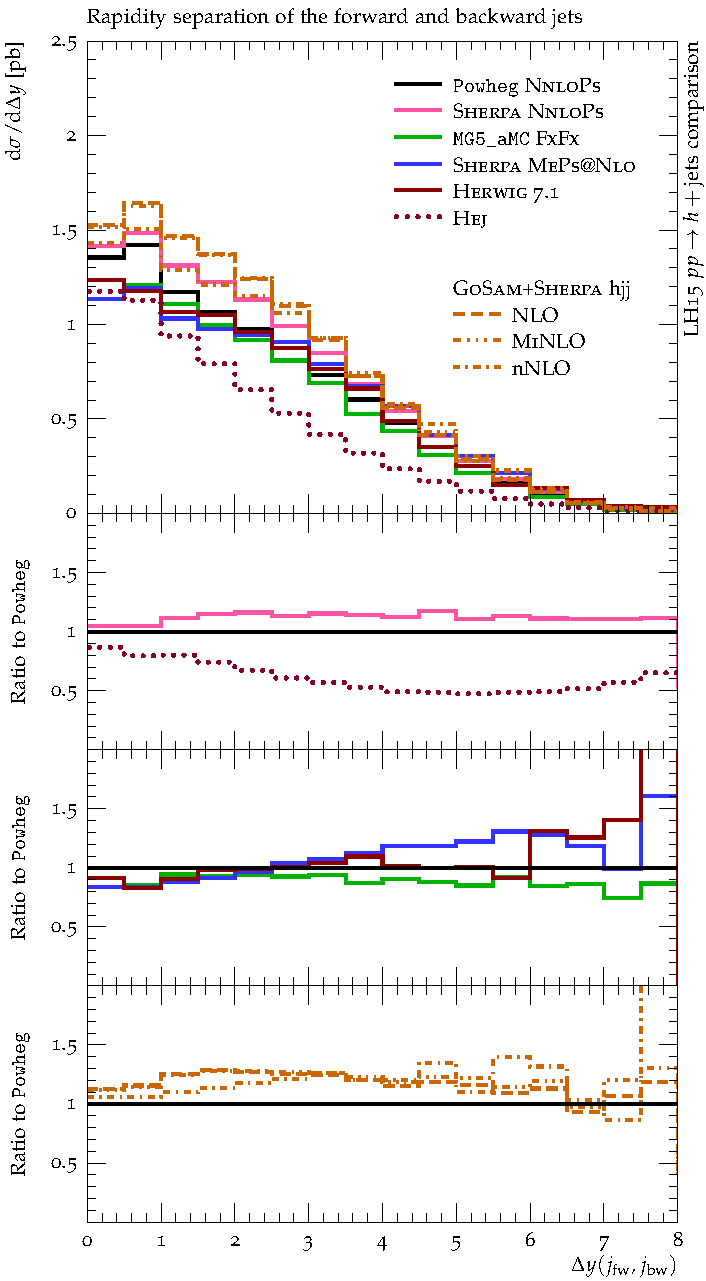
\includegraphics[width=0.47\textwidth]{figures/hjetscomp_u_jjdy_dy.pdf}
  \hfill
  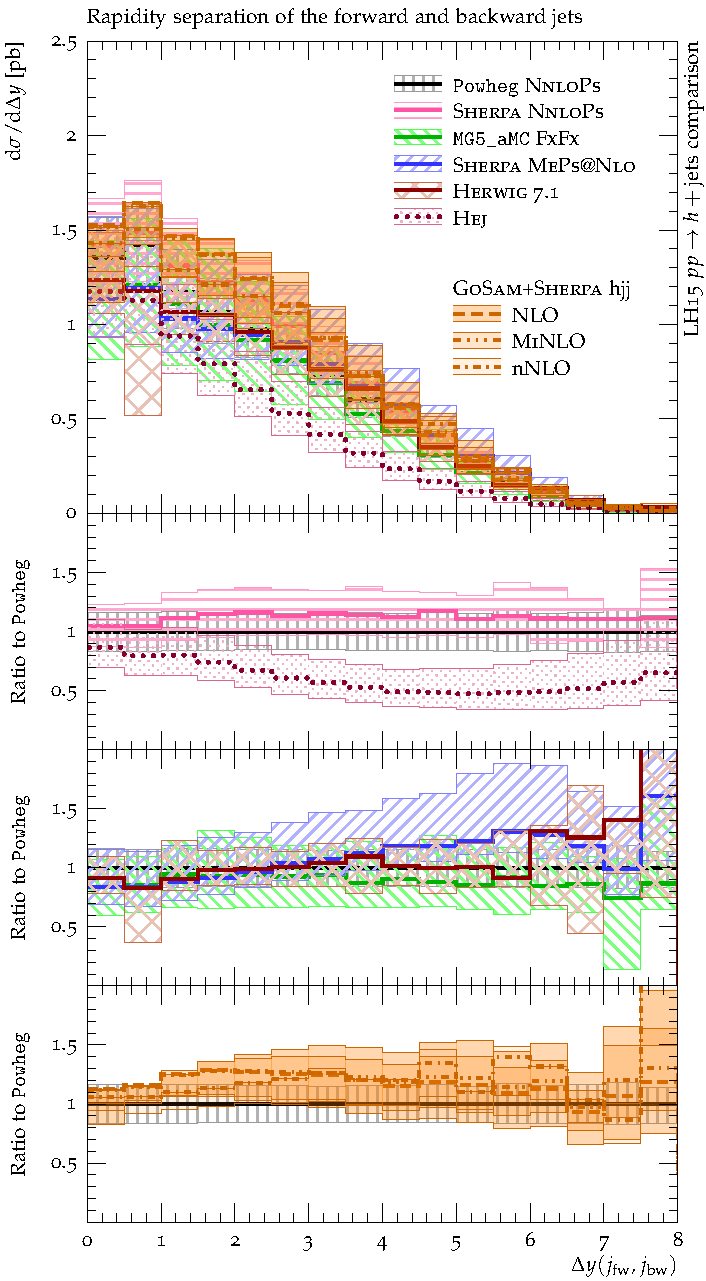
\includegraphics[width=0.47\textwidth]{figures/hjetscomp_jjdy_dy.pdf}
  \caption{\label{fig:hjetscomp:results:2obs:dyjj_fb}%
    The rapidity separation between the two jets most widely separated
    in rapidity, i.e.~the two most forward/backward jets for
    $h\,+\!\ge\!2$-jets production, shown without (left) and with
    (right) uncertainties. The plot layout is the same as the one used
    in Figure~\ref{fig:hjetscomp:results:2obs:hpt}.}
\end{figure}

As a short digression, it is interesting to consider the rapidity 
separation of the most forward and backward jets, instead of the two
leading jets. Of course, only that fraction of dijet events which are accompanied by 
a third (or more) jet (i.e.~three-jet events) result in 
a different value for this observable, as compared to $\Delta
y(j_1,j_2)$ for the $p_\perp$ ordered case. It is argued that
additional jet production in such rapidity ordered states is well
described by calculations incorporating BFKL effects.
The overall pattern of results between the $p_\perp$ and rapidity
ordered case is the same; certainly, the latter selection leads to a
wider $\Delta y$ distribution. In more detail,
Figure~\ref{fig:hjetscomp:results:2obs:dyjj_fb} shows a somewhat
different relative and absolute behavior of the various calculations.
\Powheg \NNLOPS here tends to generate slightly more 
central jets than the other calculations, while the opposite is true 
for \Sherpa \MEPSatNLO, which exhibits a clear slope wrt.~\Powheg. Again,
for \Sherpa \MEPSatNLO, this behavior can be traced back to \Sherpa \MEPSatNLO using its parton
shower in the scale setting procedure for forward jet production. 
The fixed order calculations of \GoSam{}+\Sherpa now possess a small
shape difference compared to the \Powheg reference, which was not
present in the leading jets version of this observable. On the
other hand, \Hej produces the same relative shape that it showed in the 
leading jets case, up to rapidity separations of around $4$. For
larger rapidity differences, it moves closer to
the reference prediction, being 30\% below the reference at
$\Delta y=8$. Taking the assumption that  \Hej provides the best description in
this kinematic regime  at face value, all DGLAP based parton shower 
resummations, as well as fixed order calculations, predict 
cross sections that are too large at large rapidity intervals.

\begin{figure}[t!]
  \centering
  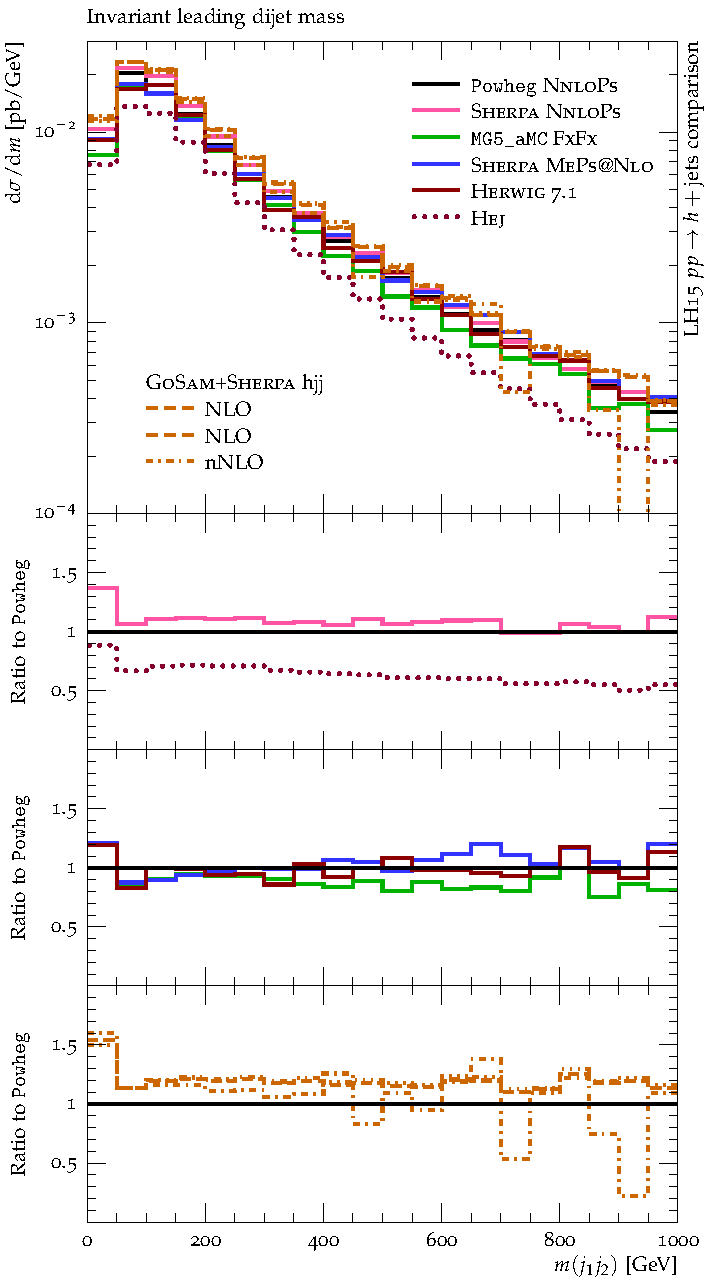
\includegraphics[width=0.47\textwidth]{figures/hjetscomp_u_dijet_mass.pdf}
  \hfill
  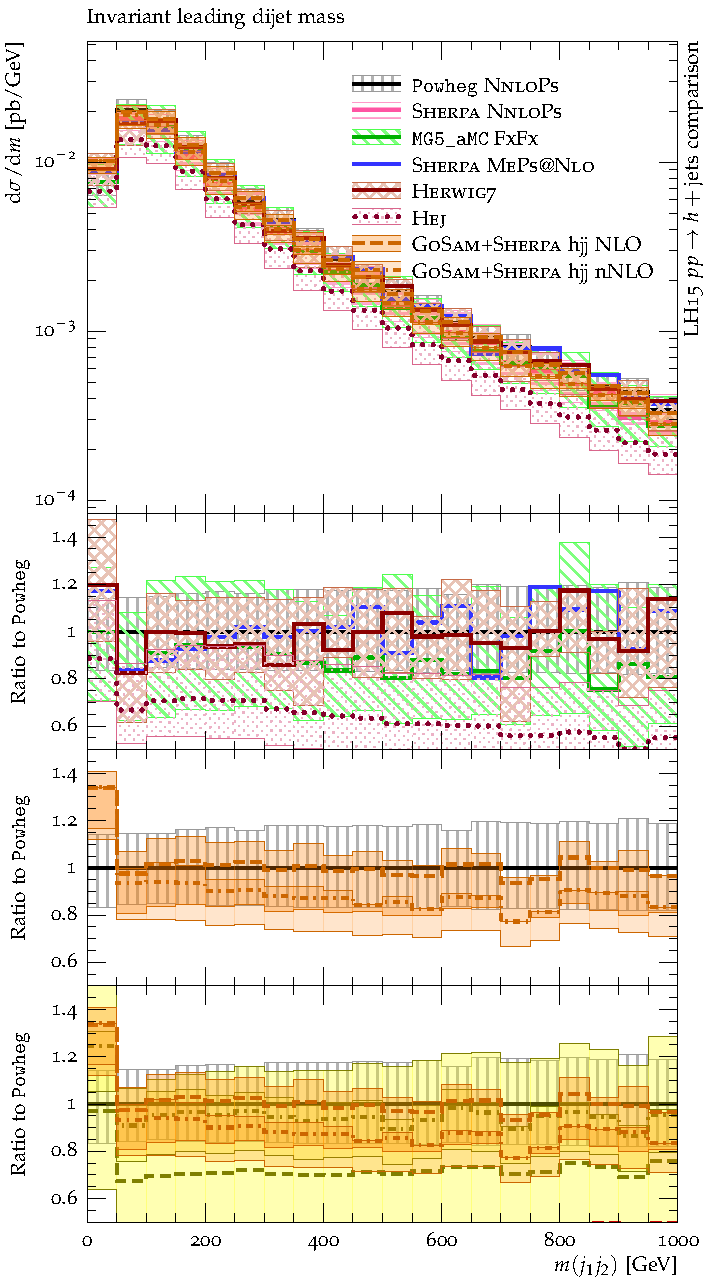
\includegraphics[width=0.47\textwidth]{figures/hjetscomp_dijet_mass.pdf}
  \caption{\label{fig:hjetscomp:results:2obs:mjj}%
    The invariant mass distribution of the leading dijet system in
    $h\,+\!\ge\!2$-jets production, shown without (left) and with (right)
    theoretical uncertainties. The plot layout is the same as the one
    used in Figure~\ref{fig:hjetscomp:results:2obs:hpt}.}
\end{figure}

Similar conclusions as for Figure~\ref{fig:hjetscomp:results:2obs:dyjj} 
hold for for the dijet invariant mass distribution formed by the 
leading jets, although the differences among predictions are smaller.
In fact, Figure~\ref{fig:hjetscomp:results:2obs:mjj} shows that there
are almost no shape deviations among the various predictions, except
for the first-to-second bin transition, which \Powheg and \MGaMC
predict to rise more strongly. All other deviations are mainly driven
by rate differences. \Sherpa \NNLOPS is larger than \Powheg \NNLOPS
by about 10\%, and maintains this excess almost throughout the whole
range. The multijet merged calculations are also in good agreement
with the \Powheg reference and, more importantly, with one another. Only
\MGaMC falls below \Herwig and \Sherpa \MEPSatNLO, being about 20\%
lower at $1\tev$, but well within the uncertainties of the other
calculations. The \GoSam{}+\Sherpa NLO calculations display the same
increase of the cross section wrt.~the reference as seen before -- a
constant 20\% increase. The scale variations in all three methods,
pure NLO, \Minlo and \Loopsim, are also in agreement for this
observable. Only \Loopsim suffers somewhat from the limited statistics
of its NLO $hjjj$ component. Again, \Hej deviates more strongly,
but this time mainly as a result of its LO normalization, being a
near constant $\sim 40\%$ below the other predictions.

\begin{figure}[t!]
  \centering
  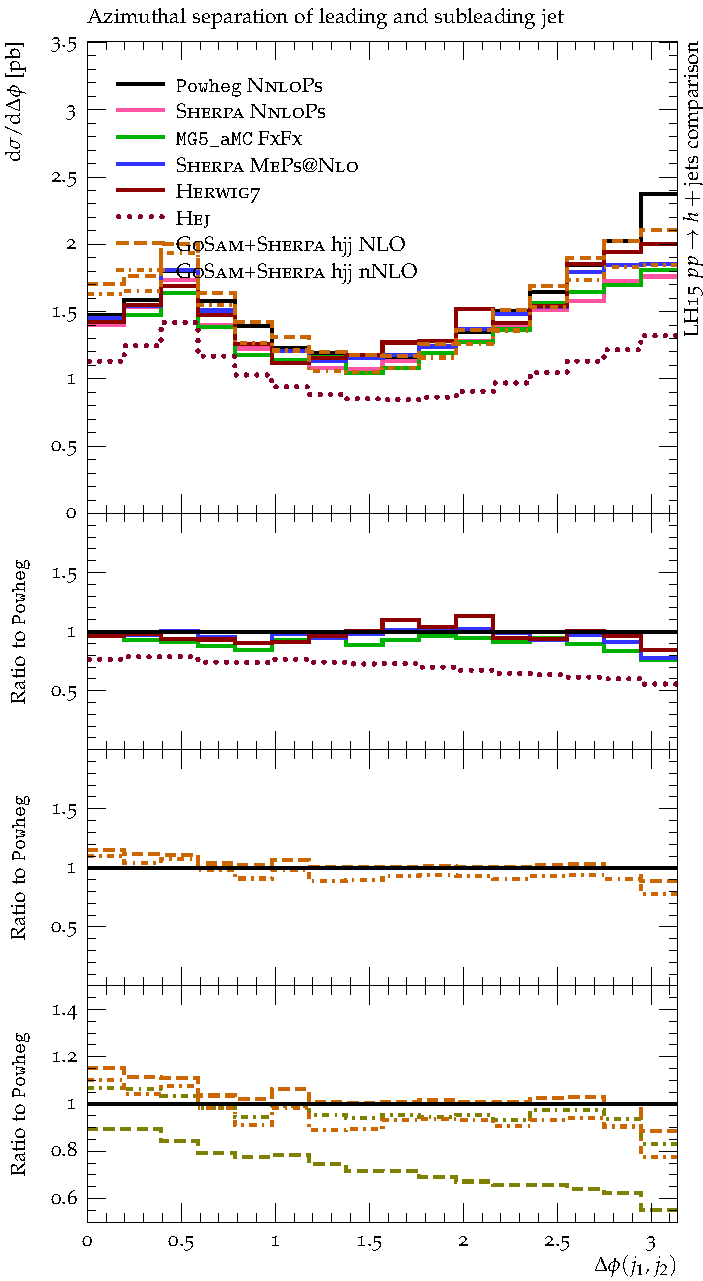
\includegraphics[width=0.47\textwidth]{figures/hjetscomp_u_deltaphi_jj_incl.pdf}
  \hfill
  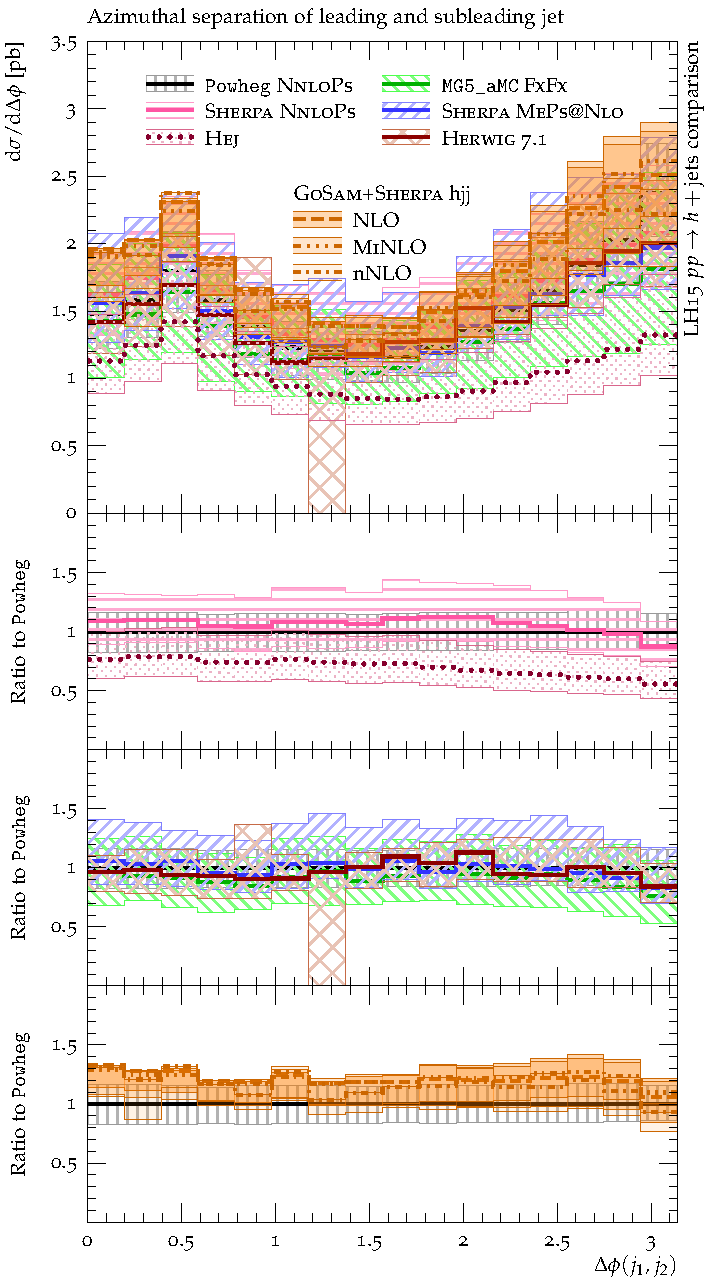
\includegraphics[width=0.47\textwidth]{figures/hjetscomp_deltaphi_jj_incl.pdf}
  \caption{\label{fig:hjetscomp:results:2obs:dphijj}%
    The azimuthal angle separation, $\Delta\phi(j_1,j_2)$, between the
    two leading jets for $h\,+\!\ge\!2$-jets production, presented
    without (left) and with (right) the associated theoretical
    uncertainties. Again, the plot layout is the same as the one used in
    Figure~\ref{fig:hjetscomp:results:2obs:hpt}.}
\end{figure}

As a last multi-object observable, we examine the azimuthal separation of 
the leading dijet pair. Although this observable plays a crucial role 
only after VBF selection cuts are made,  it is interesting to analyze this
observable for the inclusive dijet selection in order to judge which features
are impressed upon it by the VBF event selection.
Inherent differences in the description on the inclusive level will
invariably feed through to the VBF analysis level, and will then be
overlayed with the cut efficiency effects of the various calculations.
The observable possesses two topologically distinct regions. In the
first at $\Delta\phi\gtrsim0$, both jets are in the same azimuthal
hemisphere and recoil against the Higgs boson plus softer radiation
(including further jets if present). 
For this configuration, larger
parton shower effects are expected.
%and a peak at the jet
%threshold will form. JH: don't know what this means
Conversely, for $\Delta\phi\lesssim\pi$, both jets are back-to-back,
recoiling against each other -- but they do not necessarily have to be
$p_\perp$ balanced. In this situation, the Higgs boson will
mostly have small-sized to medium-sized transverse momentum.
While the Higgs boson's transverse momentum is affected by parton
showering off these topologies, the $\Delta\phi$ distribution is more
robust regarding these corrections.
The various predictions for the $\Delta\phi$ separation between the
two leading jets are shown in Figure~\ref{fig:hjetscomp:results:2obs:dphijj},
and are found to be in reasonable agreement with each other,
neglecting for a moment the lower rate of \Hej due to the LO
normalization. \Hej
features a roughly 20\% smaller cross section for small $\Delta\phi$,
which increases to about 40\% in the dijet back-to-back region.
\Sherpa \NNLOPS exhibits again a larger cross section,
$\mathcal{O}(15\%)$ for $\Delta\phi\lesssim2.5$, when compared to the
\Powheg \NNLOPS result. It agrees with \Powheg \NNLOPS  in the dijet back-to-back
region. All multijet merged distributions agree very well with each
other and the reference. The same applies to the various
\GoSam{}+\Sherpa NLO calculations; they agree very well among
themselves, despite their different scales and inputs, but exhibit a
20\% higher rate wrt.~the reference for $\Delta\phi>0.5$, which
increases to 30\% as $\Delta\phi\to0$. 
There is one feature of the \Powheg reference that stands out from the
crowd of other predictions, which is that it rises more strongly
than the others towards the $\Delta\phi=\pi$ limit. The shape change
wrt.~\Hej is however fairly mild. Recalling that the second jet is
only described at LO in \Powheg, it is more than plausible that any
NLO treatment will depopulate this area to some extent. As for the
case of \Sherpa \NNLOPS, it is more subtle, but the reason for the
different behavior, as before, lies in the choice of 
scales. Again, the example of the $p_\perp$ balanced jet topologies and
their scale setting, which we discussed for the $p_\perp(h)$
distribution in the $n_j\ge2$-jet bin, can be used to understand why
\Sherpa's \NNLOPS generates this different behavior in this region.



\subsubsection{VBF observables}
\label{sec:hjetscomp:results:VBFobs}

A situation where Higgs boson production through gluon fusion primarily
serves as a background is found in analyses intended to measure its
couplings to weak vector bosons. To enhance the relative contribution
of processes where the Higgs boson production proceeds through weak
vector boson fusion (VBF), additional cuts are placed on the so-called
tagging jets. The tagging jets themselves can now be defined in
multiple ways. In the study performed during the Les Houches 2013
workshop \cite{AlcarazMaestre:2012vp}, the standard leading
($p_\perp$-ordered) jet selection was supplemented with the
forward-backward selection defining the pair of jets with the largest
rapidity separation as tagging jets. Another strategy using the
highest invariant mass jet pair was also studied more recently
\cite{Greiner:2015jha}.

%In the present study, we generalised these 
%definitions, defining the tagging jets as the leading pair of 
%$p_\perp$-ordered jets which fulfils the thereupon applied cuts. 
%Of course, differences between the schemes only manifest themselves in 
%the presence of at least three jets and are, thus, formally of higher 
%order. Numerically, however, they can have a major impact and their 
%choice depends on the physics aims of the analysis to be performed. 

In this analysis, the leading and subleading jets are required to have
a mass greater than $400\gev$ and a rapidity separation greater than
$2.8$. This set of cuts is referred to as VBF cuts. An alternative set
of cuts (VBF2) requires that any two jets satisfy the above
requirements. For many observables, the distributions are similar for
the two cases, and only the VBF cut scenario will be presented.
%In our analysis, requiring the tagging jet invariant mass and rapidity 
%separation to be in excess of $400\,\gev$ and $2.8$, respectively, 
%prepares the typical VBF kinematics. Now, the contamination of these 
%observables with the irreducible background of Higgs produced in gluon 
%fusion is a key quantity in the accuracy of the extraction of the coupling 
%parameters. We thus proceed to analyse the congruence of the different 
%descriptions of a selection of key observables with the standard tagging 
%jet using the leading and sub-leading $p_\perp$-ordered jets.
Results for the alternative choice can be found at the project's
webpage \cite{webpage}.

%\begin{figure}[t!]
%  \centering
%  \begin{minipage}{0.47\textwidth}
%    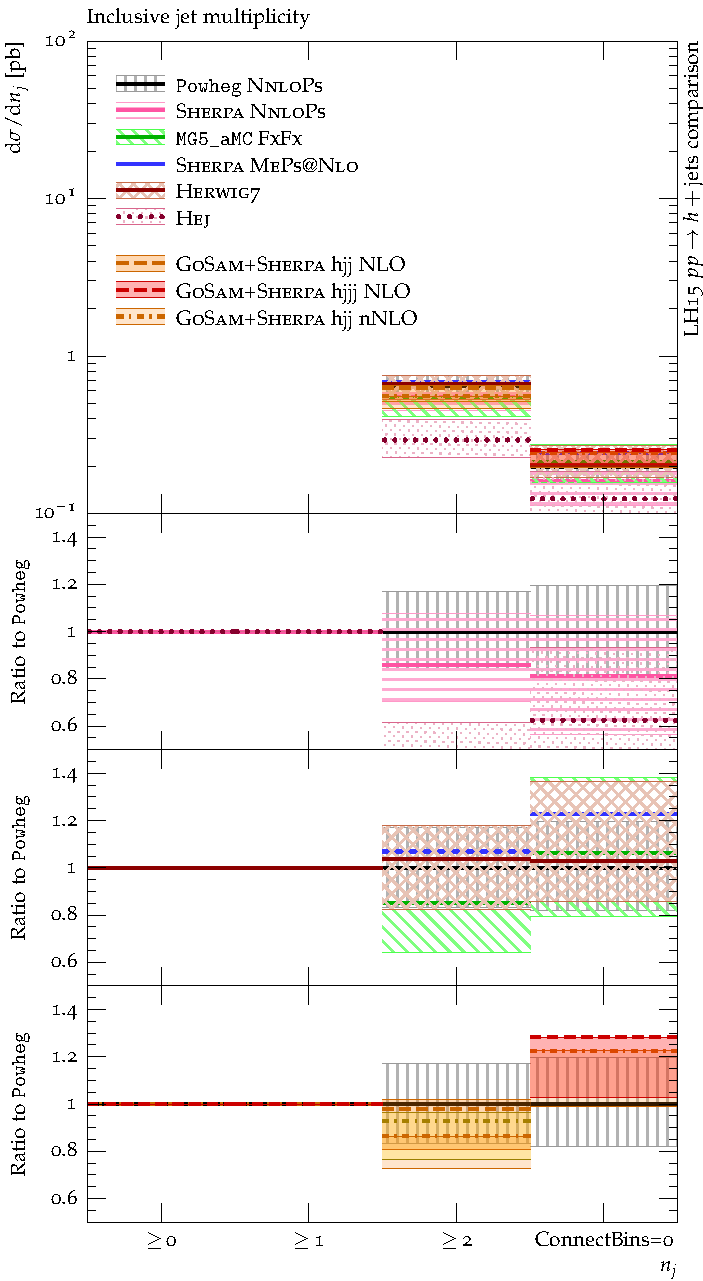
\includegraphics[width=\textwidth]{figures/hjetscomp_NJet_incl_30_VBF.pdf}
%  \end{minipage}
%  \hfill
%  \begin{minipage}{0.47\textwidth}
%    \lineskip-1.35pt
%    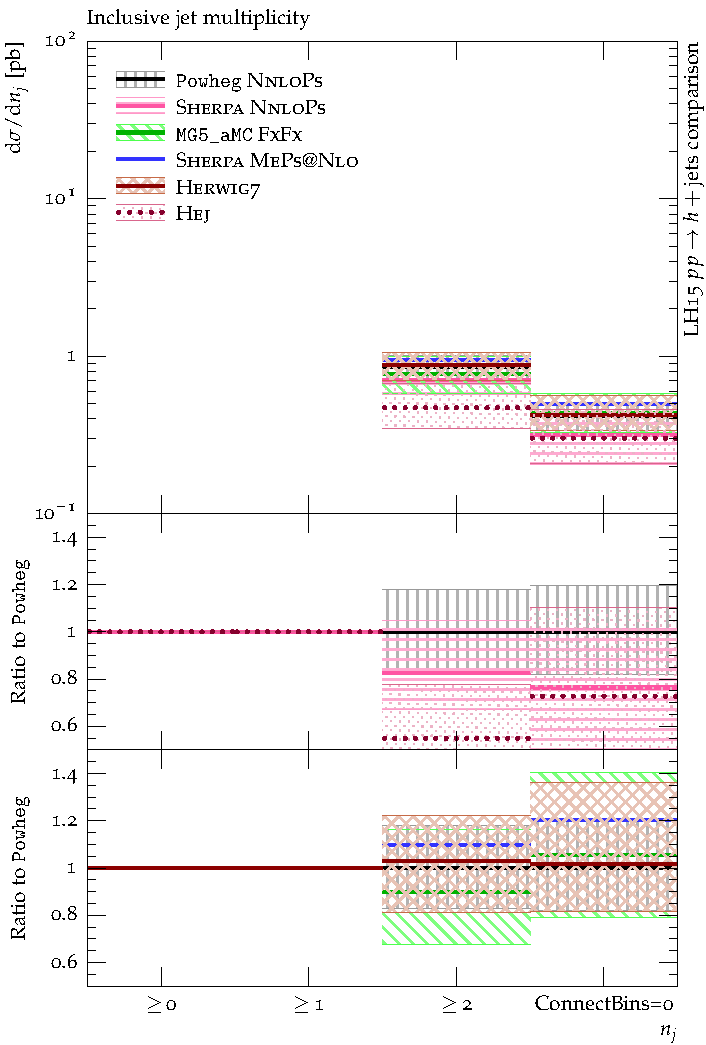
\includegraphics[width=\textwidth]{figures/hjetscomp_NJet_incl_30_VBF2.pdf}\\
%    
\includegraphics[width=\textwidth]{figures/ratiopanelplaceholder.pdf}
%  \end{minipage}
%  \caption{
%    The inclusive jet multiplicities after the application of the VBF 
%    cuts standard leading tagjet definition (VBF, left) and 
%    the generalised leading tagjet definition (VBF2, right).
%    \label{fig:hjetscomp:results:inclobs:njets_VBF}
%  }
%\end{figure}

\begin{figure}[t!]
  \centering
  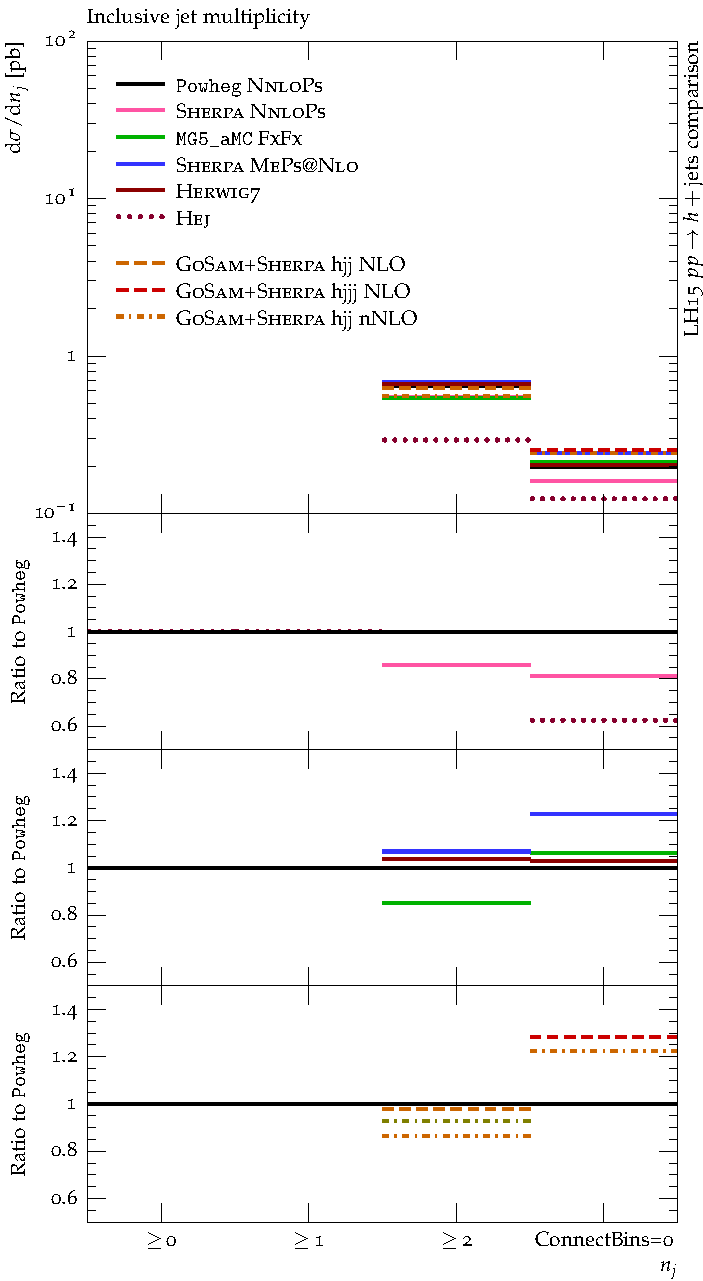
\includegraphics[width=0.47\textwidth]{figures/hjetscomp_u_NJet_incl_30_VBF.pdf}
  \hfill
  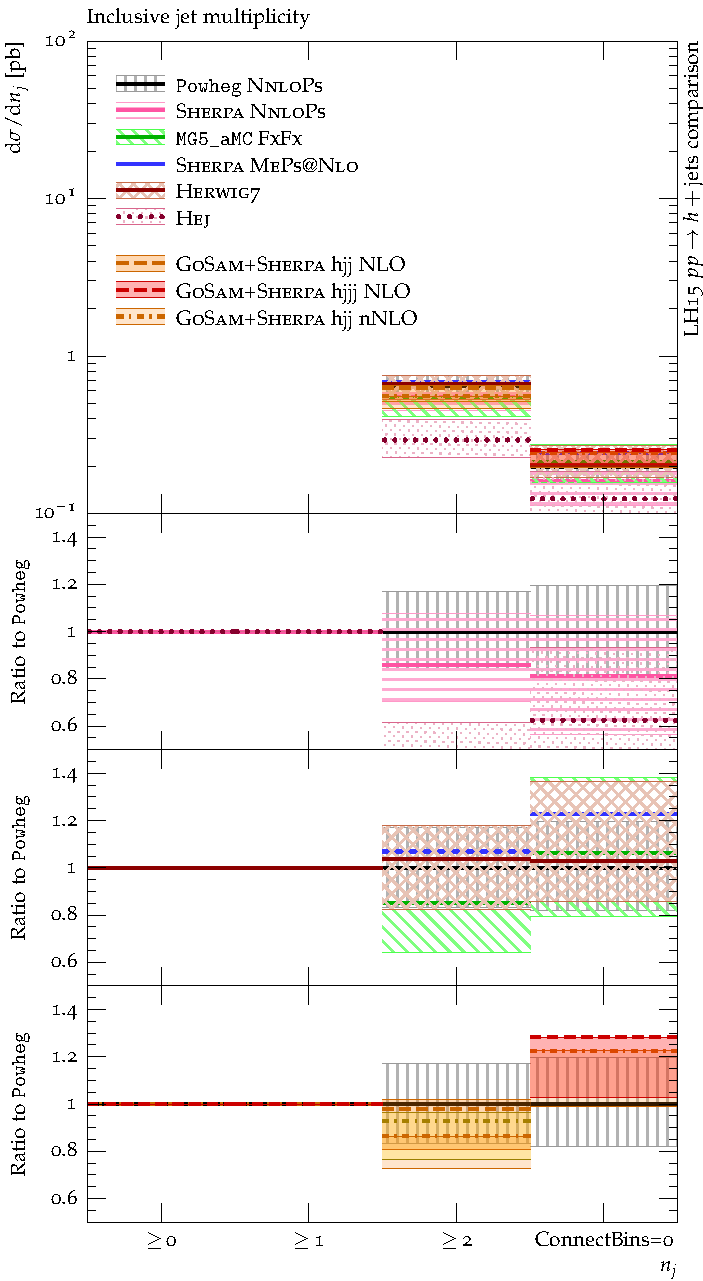
\includegraphics[width=0.47\textwidth]{figures/hjetscomp_NJet_incl_30_VBF.pdf}
  \caption{\label{fig:hjetscomp:results:inclobs:njets_VBF}%
    The inclusive jet multiplicities after imposing the leading
    tag-jets definition (see text for the details of the `VBF'
    selection), shown without (left) and with (right) uncertainties.}
\end{figure}

\begin{figure}[t!]
  \centering
  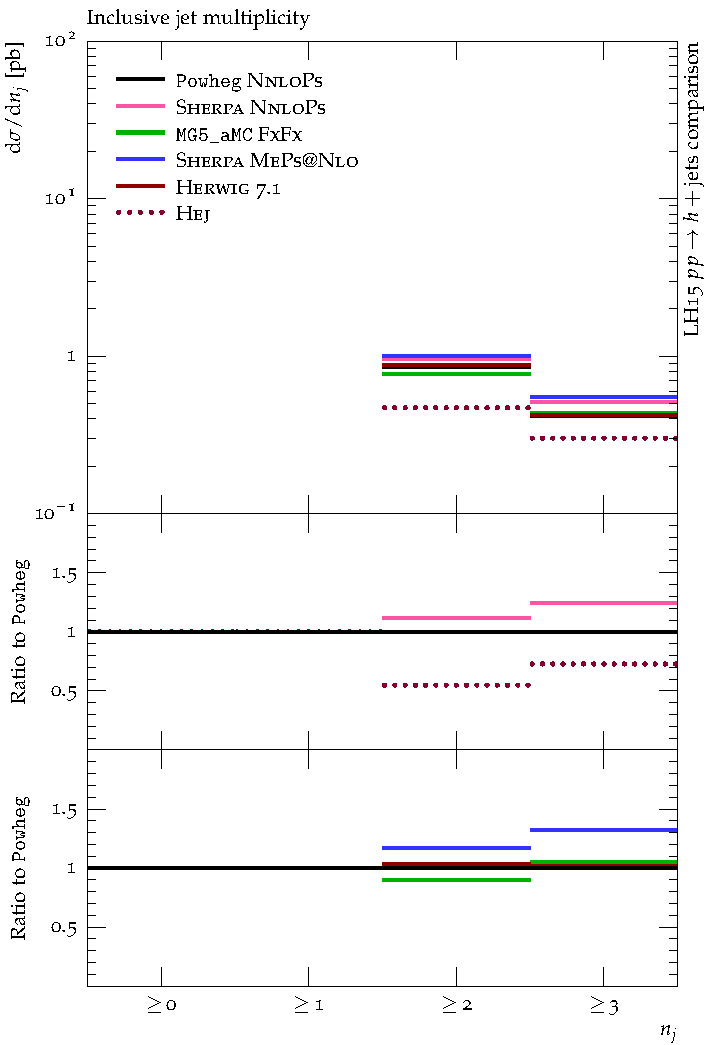
\includegraphics[width=0.47\textwidth]{figures/hjetscomp_u_NJet_incl_30_VBF2.pdf}
  \hfill
  \includegraphics[width=0.47\textwidth]{figures/hjetscomp_NJet_incl_30_VBF2.pdf}
  \caption{\label{fig:hjetscomp:results:inclobs:njets_VBF2}%
    The inclusive jet multiplicities after the application of the `VBF2'
    tag-jets cuts (see text for the definition), shown without (left)
    and with (right) uncertainties.}
\end{figure}

The inclusive jet multiplicity distributions after the application of
the VBF (VBF2) cuts are shown in
Figure~\ref{fig:hjetscomp:results:inclobs:njets_VBF}
(Figure~\ref{fig:hjetscomp:results:inclobs:njets_VBF2}).  The
hierarchy observed is essentially the same as for the inclusive jet
multiplicity distribution without any cuts. The differences among the
predictions are slightly smaller with the VBF2 cuts than with the VBF
cuts.  In both cases, the \NNLOPS calculations are again in good 
agreement, with \Sherpa \NNLOPS predicting slightly larger cross sections.
\Hej predicts only about 50\% of the cross section of \NNLOPS.
%Comparing with the inclusive dijet
%cross sections of Figure \ref{fig:hjetscomp:results:inclobs:njets},
%it therefore predicts a significantly smaller VBF cut efficiency compared to 
%the \NNLOPS calculations.
For the $\ge2$-jet bin, the NLO merged predictions vary from a 20\%
smaller cross section (\MGaMC) to a 20\% larger cross section (\Sherpa
\MEPSatNLO); both are at the edge of the \NNLOPS uncertainty
band. Interestingly, their uncertainty is of similar size as \NNLOPS,
$\sim$20\%, despite being of NLO accuracy for these observables (only
LO for \NNLOPS). This hints at underestimated uncertainties of the
\NNLOPS calculations for this observable. The NLO and \Minlo
\GoSam{}+\Sherpa predictions are also 20\% larger than the \NNLOPS
result in the $\ge2$ jet bin, close to the \Sherpa \MEPSatNLO
prediction, while the \Loopsim prediction is about 5\% higher than the
\NNLOPS predictions.
More differences are apparent after requiring a third jet. The NLO and
\Minlo \GoSam{}+\Sherpa predictions are substantially larger than the
\NNLOPS predictions and the prediction from \MGaMC and \Herwig, but in better
agreement with that from \Sherpa \MEPSatNLO. This is expected given
the NLO normalization present in those calculations (NLO,\Minlo
\GoSam{}+\Sherpa, \Sherpa \MEPSatNLO). The third jet arises from parton
showering in the \NNLOPS calculations and from the parton shower matched 
leading order matrix elements in \MGaMC and \Herwig. Owing to the  
matching techniques employed and the  resummation uncertainties that have not been evaluated, 
the uncertainties are underestimated in both calculations. The same 
therefore holds for \Powheg \NNLOPS and (partially) for \Sherpa 
\NNLOPS. 

\begin{figure}[t!]
  \centering
  \includegraphics[width=0.47\textwidth]{figures/hjetscomp_u_deltaphi_jj_VBF.pdf}
  \hfill
  \includegraphics[width=0.47\textwidth]{figures/hjetscomp_deltaphi_jj_VBF.pdf}
  \caption{\label{fig:hjetscomp:results:VBFobs:dphijj}%
    The azimuthal separation of the leading jet pair (VBF cuts) shown
    without (left) and with (right) uncertainities in $h\,+\!\ge\!\!2$-jet
    production.}
\end{figure}

The azimuthal separation between the two tagging jets is a crucial
observable in VBF measurements. In general, there is good agreement 
among the various predictions for this observable, with the caveat
that \Sherpa, in both its \NNLOPS and its \MEPSatNLO forms, predicts a
shallower dip at $\Delta\phi(j_1,j_2)\approx\tfrac{\pi}{2}$, something
that can be traced to its parton shower. Similar distributions (and
agreement) are observed if the generalised tagging jet definition
(VBF2) is used.

%% \begin{figure}[t!]
%%   \centering
%%   \includegraphics[width=0.47\textwidth]{figures/hjetscomp_u_deltaphi2_VBF.pdf}
%%   \hfill
%%   \includegraphics[width=0.47\textwidth]{figures/hjetscomp_deltaphi2_VBF.pdf}
%%   \caption{
%%     Azimuthal separation of the leading jet pair (left) and 
%%     $\Delta\phi_2$ (right) after applying VBF cuts in $H+\ge2$ jet
%%     production.
%%     \label{fig:hjetscomp:results:VBFobs:phi2}
%%   }
%% \end{figure}



\subsubsection{Multijet observables}
\label{sec:hjetscomp:results:mjobs}

In this section we consider observables sensitive to more than two jets.
The most accurate predictions here come from the NLO computations of 
\GoSam{}+\Sherpa and \Sherpa \MEPSatNLO both of which include the 3rd 
jet at NLO accuracy and the 4th jet at LO accuracy. \MGaMC and \Herwig 
both include the 3rd jet at LO while the 4th jet is LO in \Herwig but 
showered in \MGaMC. \Hej also includes LO matrix elements for the production 
of the thirf jet. The \NNLOPS codes only have parton shower accuracy 
throughout the observables of this section.


\begin{figure}[t!]
  \centering
  \includegraphics[width=0.47\textwidth]{figures/hjetscomp_u_H_jjj_pT_incl.pdf}
  \hfill
  \includegraphics[width=0.47\textwidth]{figures/hjetscomp_H_jjj_pT_incl.pdf}
  \caption{
    The Higgs boson transverse momentum in the presence of at least three 
    jets, shown without (left) and with (right) theoretical uncertainties.
    \label{fig:hjetscomp:results:mobs:hpt_j3}
  }
\end{figure}

The Higgs boson transverse momentum distribution for $h\,+\!\ge\!\!3$ jets is shown in
Figure~\ref{fig:hjetscomp:results:mobs:hpt_j3}. In general we see larger
results from predictions with at least LO accuracy over \Powheg, which includes
the 3rd jet via the parton shower. The \Sherpa \NNLOPS result is also
significantly larger than \Powheg which shows that the \Sherpa shower generates
more radiation than \Pythia~8. The \Hej prediction begins to increase over
\Powheg at high $p_T$ and is closer there to the NLO results of \GoSam{}+\Sherpa and
\Sherpa \MEPSatNLO. The multijet merged calculations on the whole agree well
within scale uncertainties, though these are rather large for \MGaMC, and the
central value for \Herwig shows a clear deviation below the jet $p_T$ cut. The
benefit of NLO accuracy is clearly seen in the \GoSam{}+\Sherpa result, which has large
corrections with respect to  \Powheg. The \Minlo scale choice used in the fixed order
computation has a central value that is almost identical to the dynamical scale
of $\tfrac{1}{2}\,\sqrt{m_{h}^2+\sum p_{T,j_i}^2}$. The scale variations
however are much smaller than the fixed order NLO.

\begin{figure}[t!]
  \centering
  \includegraphics[width=0.47\textwidth]{figures/hjetscomp_u_jet3_pT_incl.pdf}
  \hfill
  \includegraphics[width=0.47\textwidth]{figures/hjetscomp_jet3_pT_incl.pdf}
  \caption{
    The third jet transverse momentum distribution for $H+\ge3$ jets
    shown without (left) and with (right) theoretical uncertainty bands.
    \label{fig:hjetscomp:results:mobs:j3pt}
  }
\end{figure}

The third jet $p_T$ for $h\,+\!\ge\!\!3$ jets is shown in
Figure~\ref{fig:hjetscomp:results:mobs:j3pt}. Overall, a similar pattern to the
previous Higgs boson transverse momentum distribution is followed. \Sherpa
\MEPSatNLO has a much smaller scale uncertainty than \MGaMC, which mirrors 
the small scale uncertainty of the NLO \GoSam{}+\Sherpa calculation. The fixed
order \GoSam{}+\Sherpa results show more than a 50\% increase over \Powheg at large
$p_T$.  The close agreement between central values of \GoSam{}+\Sherpa using the
dynamical scale of $\tfrac{1}{2}\,\sqrt{m_{h}^2+\sum p_{T,j_i}^2}$, and \Minlo
is somewhat suprising. The \Minlo results again show a significant decrease in
scale variations - particularly at high $p_T$. Care
should be taken in interpreting the high $p_T$ region since due to the
complexity of the phase space, the MC statistical error is beginning to come into
play.

%\begin{figure}[t!]
%  \centering
%  \includegraphics[width=0.47\textwidth]{figures/hjetscomp_u_HT_all.pdf}
%  \hfill
%  \includegraphics[width=0.47\textwidth]{figures/hjetscomp_HT_all.pdf}
%  \caption{
%    The $H_T$ distribution for $H+\ge1$ jets \Todo{is this correct?}
%    without (left) and with (right) uncertainties.
%    \label{fig:hjetscomp:results:mobs:HT_all}
%  }
%\end{figure}

\begin{figure}[t!]
  \centering
  \includegraphics[width=0.47\textwidth]{figures/hjetscomp_u_HT_jets.pdf}
  \hfill
  \includegraphics[width=0.47\textwidth]{figures/hjetscomp_HT_jets.pdf}
  \caption{
    The $H_{T,\mathrm{jets}}$ distribution for $H+\ge1$ jet final
    states, without (left) and with (right) uncertainties.
    \label{fig:hjetscomp:results:mobs:HT_jets}
  }
\end{figure}

%The $H_T$ distribution (sum of the transverse momenta for all objects in the
%final state) for $H+\ge1$ jets is shown in
%Figure~\ref{fig:hjetscomp:results:mobs:HT_all} and the $H_T$ distribution for
%jets only is shown in in Figure~\ref{fig:hjetscomp:results:mobs:HT_jets}.

The $H_T^\text{jet}$ distribution, defined as sum scalar sum of all jet 
transverse momenta, is shown in Figure~\ref{fig:hjetscomp:results:mobs:HT_jets}. 
Requiring $h\,+\!\ge\!\!1$-jet final states this observable is
extremly sensitive to additional radiation and is a useful case to observe
the impact of different jet multiplicities. While the \NNLOPS 
computations of \Sherpa and \Powheg deviate significantly for 
$150 < H_T^\text{jet} < 600$, \Sherpa \NNLOPS agrees better with 
the BFGLP $hj$ NNLO fixed order prediction and, to a certain extent, 
the \Sherpa \MEPSatNLO computation. \Herwig and \MGaMC give results 
consistent with \Powheg except for deviations at low energies but with 
relatively large errors.

For very high $H_T^\text{jet}$ all tools including some approximation to the 3rd
jet converge, while NLO predictions for $h+1$ jet quickly begin to fall away
from the other predictions. The \Loopsim $h+(1,2)$ jet prediction at nNLO does a good
job of matching the complete NNLO result here, as it is designed to do. One also
clearly sees the benefit of the 3rd jet at NLO accuracy.  The scale variations
for the NLO $h+3$ jet cross section,  either at fixed order with \Loopsim or  with the \Minlo
procedure or with the fully merged prediction with \Sherpa \MEPSatNLO, have
significantly smaller errors above $400$ GeV than the other predictions.



\clearpage
\subsubsection{Jet veto cross sections}
\label{sec:hjetscomp:results:jvobs}


In this section, we investigate jet veto cross sections, where the phase space for
additional gluon radiation is suppressed by means of a jet veto. 
%This section is concerned with the cummulative jet veto cross sections. 
In  Figures 
\ref{fig:hjetscomp:results:jvobs:jvxs0}-\ref{fig:hjetscomp:results:jvobs:jvxs1j200}, 
additional radiation has been vetoed by the application of a maximal transverse 
momentum for the (sub)leading jet, $p_\perp^\text{veto}$. The observables plotted
in the figures recover the respective inclusive cross sections as 
$p_\perp^\text{veto}\to\infty$. In this region, the fixed order 
part of the respective calculations dominates the cross section 
and associated uncertainties. The opposite regime, where $p_\perp^\text{veto}\to 0$, 
is a classic example of a resummation-dominated observable. Here, the 
properties of the respective parton showers come fully into play and 
differences are largely due to their separate characteristics. 
%The last case 
%investigated is cross section after VBF cuts when vetoing additional 
%central jet activity in dependence of the rapidity distance of the 
%tagging jet pair, $y_\text{dist}<y_\text{dist}^\text{max}$. Here, 
%DGLAP-type resummation regions are present throughout the spectrum and 
%this observable should be ideal to study BFKL-like dynamics.

\begin{figure}[t!]
  \centering
  \includegraphics[width=0.47\textwidth]{figures/hjetscomp_u_xs_jet_veto_j0.pdf}
  \hfill
  \includegraphics[width=0.47\textwidth]{figures/hjetscomp_xs_jet_veto_j0.pdf}
  \caption{
    The exclusive zero jet cross section as a function of 
    the vetoed minimal leading jet transverse momentum,
    without (left) and with (right) uncertainties.
    \label{fig:hjetscomp:results:jvobs:jvxs0}
  }
\end{figure}

We start by considering 
the cross section for the production of a Higgs boson and no 
additional jets, as a function of the minimum jet transverse momentum 
as shown in Figure~\ref{fig:hjetscomp:results:jvobs:jvxs0}. Remarkable 
agreement between both \NNLOPS simulations and the dedicated resummation 
calculation of STWZ is found, typically better than 5\% within the considered range. 
However, as the resummation accuracy for both \NNLOPS' implementations is limited by their parton 
shower's accuracy and they do not (\Powheg) or only partially (\Sherpa) 
assess their intrinsic resummation uncertainties and the interplay with the hard process 
scale variations, their uncertainties are less well-determined than those of STWZ. Although
the uncertainties for STWZ are similar to those of the \NNLOPS predictions for low values of the
jet veto transverse momentum, they are significantly smaller for higher values, perhaps reflecting the
effects of the $\pi^2$ resummation effects included in STWZ.
 The multijet merged predictions have a wider variation, and have veto cross sections lower than
those provided by the STWZ and the NNLOPS predictions. In addition to 
suffering from their NLO normalisation in the $p_\perp^\text{veto}\to\infty$ 
limit, they also show different behavior as $p_\perp^\text{veto}\to 0$. For example, 
\Sherpa \MEPSatNLO exhibits more QCD activity than the other computations. 

\begin{figure}[t!]
  \centering
  \includegraphics[width=0.47\textwidth]{figures/hjetscomp_u_xs_jet_veto_j1_30.pdf}
  \hfill
  \includegraphics[width=0.47\textwidth]{figures/hjetscomp_xs_jet_veto_j1_30.pdf}
  \caption{
    The cross section for events containing a Higgs boson 
    and one jet with $p_\perp>30\,\gev$ as a function of
    the vetoed minimal second jet transverse momentum without
    (left) and with (right) uncertainties.
    \label{fig:hjetscomp:results:jvobs:jvxs1j30}
  }
\end{figure}

\begin{figure}[t!]
  \centering
  \includegraphics[width=0.47\textwidth]{figures/hjetscomp_u_xs_jet_veto_j1_200.pdf}
  \hfill
  \includegraphics[width=0.47\textwidth]{figures/hjetscomp_xs_jet_veto_j1_200.pdf}
  \caption{
    The cross section for events containing a Higgs boson 
    and one jet with $p_\perp>200\,\gev$ as a function of
    the vetoed minimal second jet transverse momentum without
    (left) and with (right) uncertainties.
    \label{fig:hjetscomp:results:jvobs:jvxs1j200}
  }
\end{figure}

Next, we require the presence of at least one jet with 
a minimal transverse momentum of either $30$ or $200$ \gev. 
The cross sections as a function of 
the subleading jets' maximal transverse momentum are displayed in 
Figure~\ref{fig:hjetscomp:results:jvobs:jvxs1j30} and 
Figure~\ref{fig:hjetscomp:results:jvobs:jvxs1j200} for the two lead jet cuts. 
Note that, although all parton 
shower matched or merged calculations have the same accuracy both as 
$p_\perp^\text{veto}\to\infty$ and in the resummation dominated region, 
the multijet merged calculations possess a better description of the 
second jet emission, and thus should lead to more accurate results 
throughout the spectrum, provided the merging systematics are under control. 
Currently employed uncertainty estimates, however, will not reflect this, 
as resummation uncertainties are not assessed or only incompletely assessed.

If we put no special requirements on the leading jet, cf.\ Figure 
\ref{fig:hjetscomp:results:jvobs:jvxs1j30}, good agreement 
between all calculations is found. The \NNLOPS predictions agree again within 
5\% of one another and have very similar uncertainties. This is noteworthy 
as, in comparison with the results of 
Figure~\ref{fig:hjetscomp:results:jvobs:jvxs0}, both calculations' 
accuracies have been degraded by one order. The multijet merged calculations 
show similar behavior as in the previous case: \MGaMC exhibits a smaller cross section due to 
its scale choice while \Sherpa \MEPSatNLO predicts more soft radiation. 
The relative lack of small $p_\perp$ radiation is more 
pronounced in \Herwig for this observable. Again, the uncertainties of \MGaMC and \Sherpa 
are of similar size while those of \Herwig are somewhat smaller than those of the \NNLOPS 
predictions, especially in the resummation-dominated region 
$p_\perp^\text{veto}\to 0$.

Raising the requirements on the leading jet to $200$ \gev, in Figure 
\ref{fig:hjetscomp:results:jvobs:jvxs1j200}, displays clear distinctions 
between the different calculations.  
\Sherpa \NNLOPS and \Powheg \NNLOPS have noticeably different shapes, with \Sherpa having a 
much lower cross section for low values of the subleading jet veto requirement. 
%starts out at a higher asymtotic cross section but remains within 
%20\% and of \Powheg, the respective uncertainties covering one another. 
The multijet merged calculations show \Herwig largely agreeing with 
\Powheg with a constant offset of $-10\%$, and the familiar lower 
probability of low-$p_\perp$ jet emissions. 
The asymptotic cross section for \Sherpa \MEPSatNLO is similar to that from \Sherpa \NNLOPS and, 
unsurprisingly, due to the use of the same parton shower, shows a 
similar radiation pattern. As before, it exhibits 
a relative overabundance of soft jet radiation. Lastly, the asymptotic cross section from \MGaMC 
is the same level as \Powheg's, despite 
its higher scale choice. The pattern of the uncertainties, however, 
remains the same as before.

%\Todo{The central jet veto cross sections are a mess. Looking into the 
%      analysis this is Ivan's code. It defines $y_\text{dist}$ as the 
%      minimal rapidity distance between the centre of the forward and 
%      backward jets and any jet inbetween,
%      $$
%	y_\text{dist}\;=\;\min\limits_{j|y(j_\text{bw})<y(j)<y(j_\text{fw})}
%	                  \left|y(j)-\frac{y_\text{fw}+y_\text{bw}}{2}\right|\;.
%      $$
%      It can thus take the maximum value of $4.4$. The cummulative cross 
%      section is then defined as 
%      $\sigma_2(y_\text{dist}>y_\text{dist}^\text{min})$. Thus, this 
%      observable vetoes events with too central additional radiation. 
%      It has one flaw in the implementation, however, in the absence of 
%      any third jet $y_\text{dist}$ is set to $>4.4$. Its asymtotic behavior 
%      at large $y_\text{dist}$ converges thus to the exclusive VBF 
%      cross section, instead of zero. I just do not see what kind of 
%      dynamics we are probing or what kind of relevance a construction 
%      like this has. Especially since the forward backward jet are 
%      generally not the VBF tagging jets. We do also have the same observable 
%      in the pure dijet selection, which would then at least be nicely defined. 
%      Only the effects there are even smaller. 
%      Too many cooks, I guess. One should have had a recipe first.
%      }


% \begin{figure}[t!]
%   \centering
%   \includegraphics[width=0.47\textwidth]{figures/hjetscomp_u_xs_central_jet_veto_VBF.pdf}
%   \hfill
%   \includegraphics[width=0.47\textwidth]{figures/hjetscomp_xs_central_jet_veto_VBF.pdf}
%   \caption{
%     The cross section after VBF cuts as a function of the maximal minimum 
%     rapidity distance of a central jet to the centre of the most forward 
%     and most backward jet.
%     \label{fig:hjetscomp:results:jvobs:cjvxsvbf}
%   }
% \end{figure}
% 
% \begin{figure}[t!]
%   \centering
%   \includegraphics[width=0.47\textwidth]{figures/hjetscomp_u_xs_central_jet_veto_VBF2.pdf}
%   \hfill
%   \includegraphics[width=0.47\textwidth]{figures/hjetscomp_xs_central_jet_veto_VBF2.pdf}
%   \caption{
%     The cross section after generalised VBF cuts as a function of the maximal minimum 
%     rapidity distance of a central jet to the centre of the most forward 
%     and most backward jet.
%     \label{fig:hjetscomp:results:jvobs:cjvxsvbf2}
%   }
% \end{figure}
% 
% Finally, we consider the cross section after VBF cuts applying a veto 
% on additional central jet activity with $p_\perp>30\,\gev$ in dependence 
% of the maximal rapidity distance of the tagging jets, 
% $y_\text{dist}<y_\text{dist}^\text{max}$, as displayed in 
% Figure \ref{fig:hjetscomp:results:jvobs:cjvxsvbf}. Here, all parton shower based 
% resummation calculations give very similar results with \MGaMC possessing 
% a reduced cross section due to its scale choice. \Hej, being based on 
% BFKL dynamics, does not deviate substantially in its predicted shape. 
% However, its cross section is reduced by a constant 50-60\%. Alternatively, 
% when applying the generalised version of the VBF cuts, labelled VBF2, 
% a similar picture presents itself in 
% Figure \ref{fig:hjetscomp:results:jvobs:cjvxsvbf2}. While, of course, the 
% asymtotic cross section at large $y_\text{dist}^\text{max}$ coincides with 
% the one of the standard VBF cuts, for small $y_\text{dist}^\text{max}$ the 
% generalised VBF cuts allow for a much larger cross section.



